En este capítulo se describen los principales aspectos de la solución al
problema de exploración multi-robot desarrollada\footnote{Disponible en
línea:\\
\url{https://gitlab.fing.edu.uy/federico.ciuffardi/pgmappingcooperativo}.\\ Accedido por última vez: 25/02/2022.},
incluyendo las potenciales mejoras que constituyen las contribuciones del
proyecto de grado (sección \ref{sec:cont}).

El capítulo comienza con la sección \ref{sec:hip} donde se enumeran las
hipótesis de trabajo. Luego en la sección \ref{sec:arqui} se describe la
arquitectura de la solución. Seguido de esto, en la sección \ref{sec:def} se
detallan y formalizan conceptos que son fundamentales en la solución propuesta.

Lo que resta del capítulo se dedica a profundizar en diversos aspectos de la
solución. A continuación se destacan las secciones donde se tratan las
contribuciones del proyecto. En la sección \ref{subsec:MiSimp} se describe el
método de identificación de objetivos propuesto. En la sección
\ref{subsec:MiResSub} se introduce el algoritmo de asignación de objetivos. La sección
\ref{sec:MiConstGVD} se comenta el algoritmo de
construcción incremental del GVD y la forma novedosa de tratar
las porciones desconocidas del espacio durante la construcción del GVD.
Finalmente la sección \ref{sec:miNav} se describe la planificación jerárquica
propuesta.

% En la sección \ref{sec:hip} se establecen las hipótesis asumidas para el
% desarrollo de la solución. En la sección \ref{sec:arqui} se describe al
% arquitectura de la solución. En la 
% Para el problema de asignación de objetivos (sección \ref{sec:exploracion}) se
% presentan soluciones para cada una de sus partes. Para la identificación de
% objetivos se propone una técnica novedosa basada en el rango de sensado de los
% robots que determina como objetivos a un subconjunto de los puntos fronterizos.
% La distribución de objetivos a robots, se resuelve de forma coordinada
% aplicando una variante de lo presentado en la sección \ref{subsec:wurmCoord}.

% La asignación requiere de la construcción de un mapa topológico, para esto se
% implementa la técnica descrita en la sección \ref{subsec:mapaTopGVD} que
% requiere de un GVD, el cual se construye de forma incremental con una variante
% del algoritmo \emph{brushfire dinámico} (sección \ref{subsec:constGVDInc}).

% Luego de asignado a un objetivo el robot deberá llegar hasta el, para esto es
% necesario solucionar el problema de planificación. La solución desarrollada
% aplica la idea de planificación jerárquica mencionada en la sección
% \ref{subsec:mapas}, con el motivo de permitir una planificación
% computacionalmente eficiente sin resultar en caminos innecesariamente largos.

% El problema construir el mapa de un entorno inicialmente desconocido a partir
% de los datos sensoriales de varios robots se soluciona, construyendo en cada
% robot, según la información sensorial que estos recolectan, una grilla de
% ocupación con el nodo de \gls{ROS} \emph{costmap\_2d} \cite{ROS-costmap_2d} y luego
% combinando dichas grillas con las ideas presentadas en
% \cite{stachniss2009robotic}.

\section{Hipótesis de trabajo}\label{sec:hip}
La solución se desarrolla con las siguientes hipótesis de trabajo.
\begin{enumerate}[label=(\roman*)]
  \item Cada robot puede obtener en todo momento su ubicación (posición y
    orientación) sin errores.
  \item Los robots son iguales entre sí.
  \item Las comunicaciones son ideales: sin perdida, con un ancho de banda y rango infinito.
  \item Los robots tienen la capacidad de detectar las superficies más cercanas
    que se encuentran dentro de un circulo de radio $rango$ centrado en el
    robot.
  \item El entorno a explorar es cerrado.
  \item Se conocen las dimensiones del entorno a explorar.
\end{enumerate}

% \todoremark{o capaz: se hacen con el motivo? | procuran / tienen por objeto?}
Estas hipótesis tienen el propósito de simplificar algunos aspectos del problema de
exploración permitiendo que el trabajo se pueda enfocar en otros.

La hipótesis (I) resuelve trivialmente el problema de localización \cite{slam}. 

Las hipótesis (II) y (III) simplifican la coordinación. La (II) por no tener
que hacer consideraciones especiales para cada robot. La (III) por no tener que
considerarse los posibles problemas de comunicación que pueden haber de asignar
robots a objetivos muy distantes o con obstrucciones entre sí. 

La hipótesis (IV) establece la capacidad sensorial del robot. Que sea posible 
sensar un circulo centrado en el robot, evita considerar su orientación.

La hipótesis (V) es útil para poder aplicar el criterio de parada que consiste
en detener la exploración al no tener más objetivos restantes (sección
\ref{sec:exploracion}). 

Finalmente la hipótesis (VI) permite establecer una grilla de ocupación con las
dimensiones suficientes para representar todo el entorno a explorar. 

\section{Arquitectura}\label{sec:arqui}
La arquitectura se divide en dos tipos de componentes robots y unidad central.
Existe una única unidad central que se encarga de centralizar la información
del entorno explorado y de coordinar a los multiples robots que pueden existir.
Cada componente está asociado a un hardware específico, siendo los robots móviles
y la estación central estática. 
%Los robots pueden ser uno o más mientras que la estación central es única. 
Los componentes a su vez están compuestos por módulos los cuales cuales se encargan
de tareas específicas. 

En la figura \ref{fig:arquitectura} se resume la arquitectura en un diagrama en
el cual es posible ver los componentes, sus módulos y cómo estos se distribuyen
sobre los componentes. Adicionalmente es posible apreciar una simplificación de las
comunicaciones que ocurren entre dichos módulos.


\begin{figure}[H]
  \center
  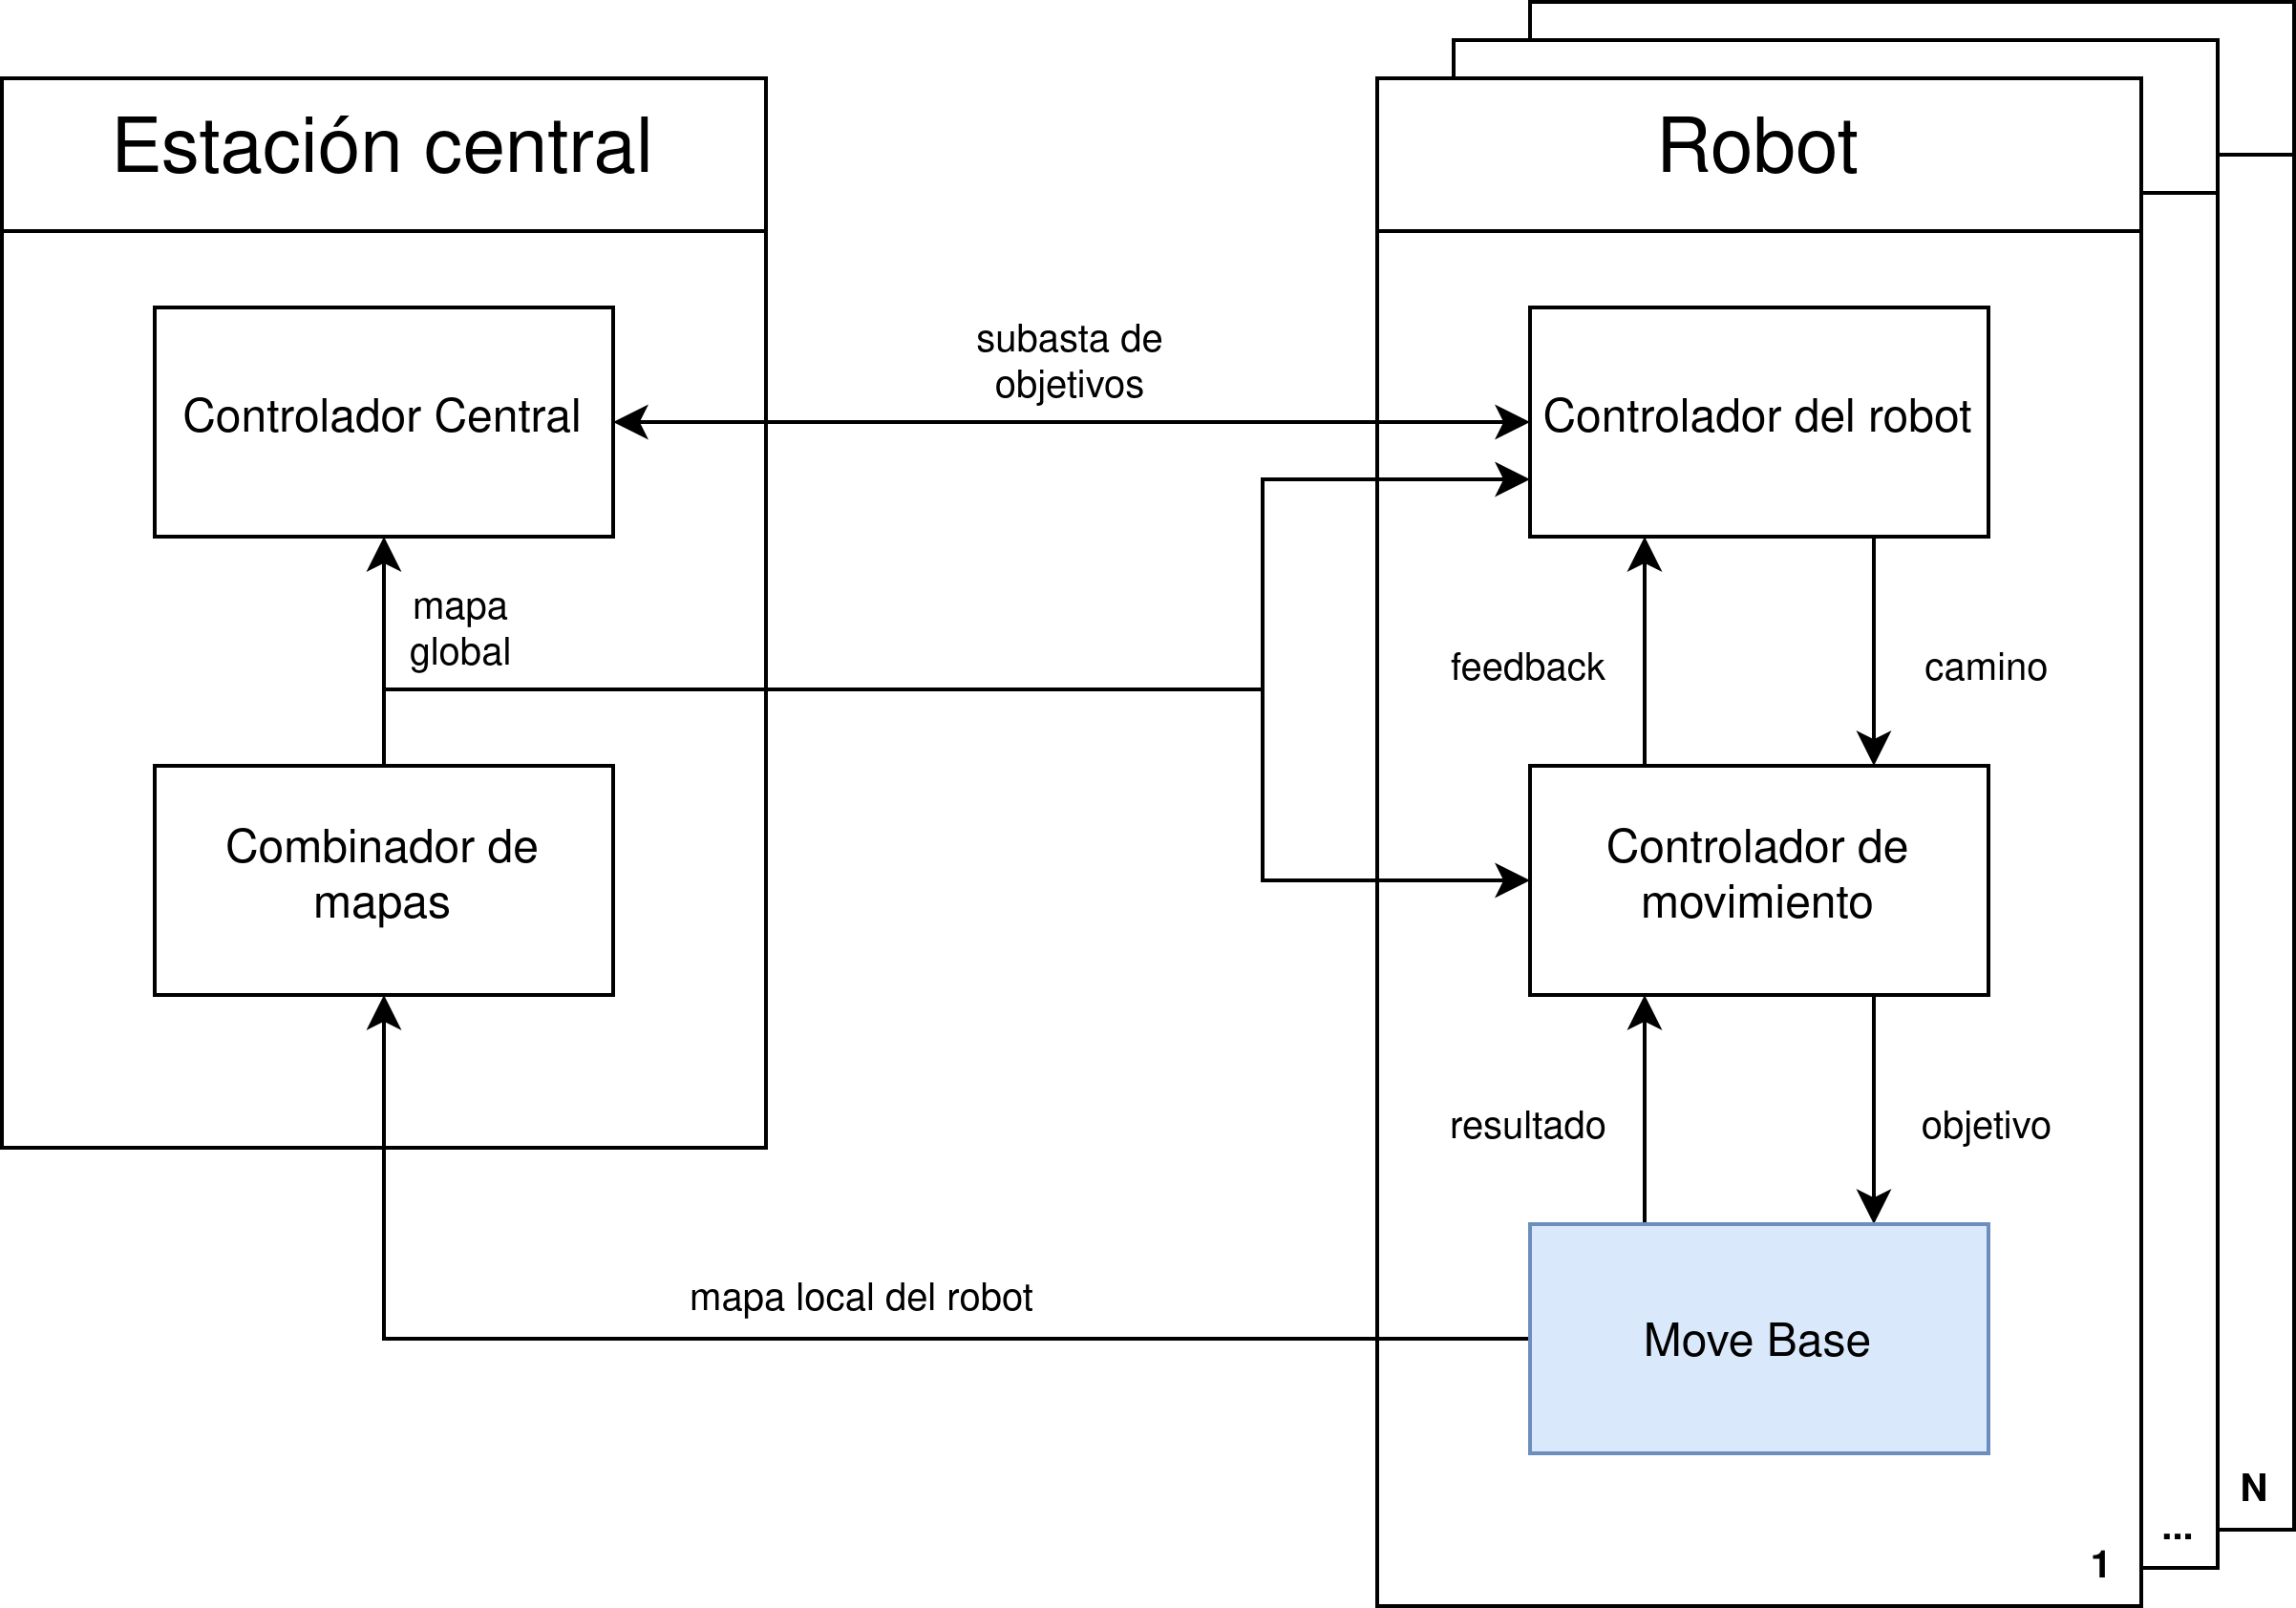
\includegraphics[width=1\linewidth]{imagenes/arquitectura.png}
  \caption[Arquitectura de la solución propuesta.]{Arquitectura de la solución propuesta. Los módulos coloreados en azul fueron implementados en este proyecto.}
  \label{fig:arquitectura}
\end{figure} 
% \todoerror[inline]{lo primero no lo entienda, lo segundo quedo?  | fig3.1: en el caption solución. colorear lo hecho con otro color}

En lo que resta de esta sección se comentará de cada módulo tanto sus tareas,
como sus interacciones con el resto de los módulos.

\subsection{Move Base}\label{subsec:move_base}
% El módulo \emph{Move Base} consiste en una instancia del nodo \gls{ROS}
% \emph{move\_base} \cite{ROS-move_base} que provee una interfaz para configurar,
% ejecutar y interactuar con el \emph{stack de navegación} de \gls{ROS}
% \cite{ROS-navigation}. 
El módulo \emph{Move Base} provee una interfaz para configurar, ejecutar e
interactuar con el \emph{stack de navegación} de \gls{ROS}
\cite{ROS-navigation}. Específicamente el módulo corresponde a un
nodo\footnote{En \gls{ROS} el concepto de nodo refiere básicamente a un proceso que
  utiliza ROS.} conocido como \emph{move\_base}
  \cite{ROS-move_base}. 

El stack de navegación de \gls{ROS} es un conjunto de nodos que tienen como propósito
que un robot pueda navegar el entorno hacia objetivos dentro del mismo. En la
figura \ref{fig:move_base} se muestra un diagrama que representa a los nodos que
componen al stack de navegación de \gls{ROS} y sus interacciones.

\begin{figure}[H]
  \center
  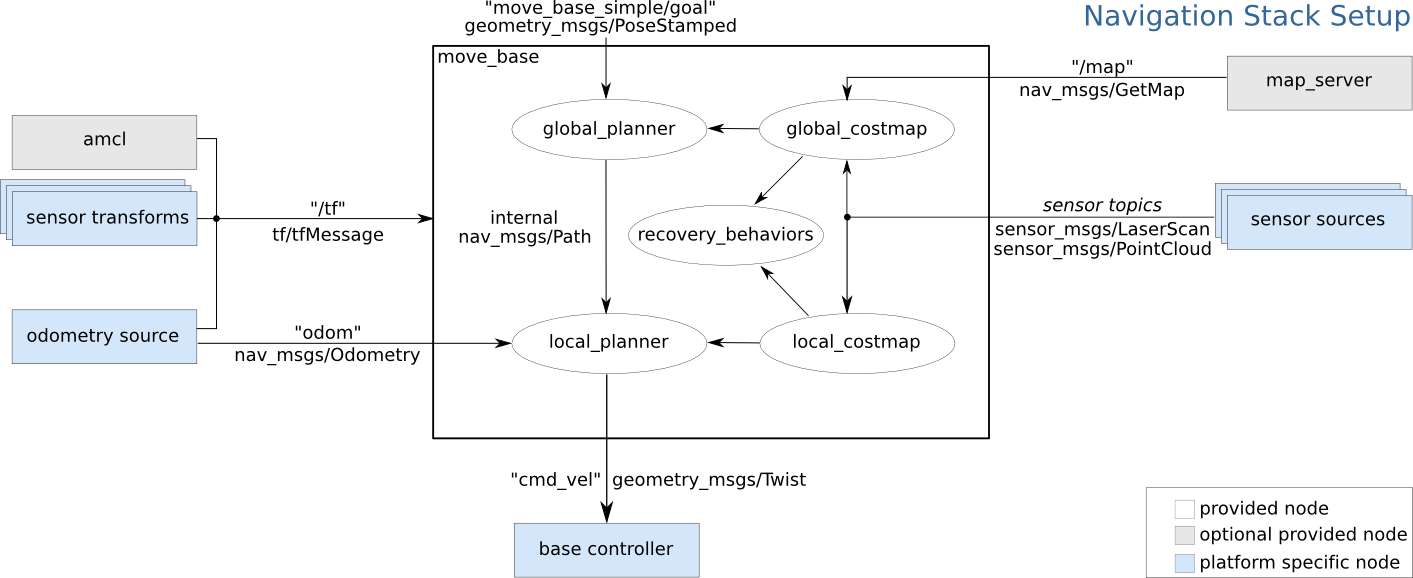
\includegraphics[width=1\linewidth]{imagenes/move_base.png}
  \caption[Arquitectura del stack de navegación de ROS.]{Arquitectura del stack de navegación de \gls{ROS}. Extraída de \cite{ROS-move_base}.}
  \label{fig:move_base}
\end{figure} 

Cuando se establece un objetivo de navegación este se trasmite al nodo
\emph{global\_planner} que se encarga de generar un plan de alto nivel
conocido como plan global, que consiste en un número de subobjetivos que al 
seguirse en secuencia llevan al objetivo.

Los subobjetivos generados por el \emph{global\_planner} son enviados al nodo
\emph{local\_planner} que se encarga de generar secuencias de velocidades
lineales y angulares que un robot debe tener a lo largo del tiempo para llegar
sin colisiones a los subobjetivos recibidos. A dicha secuencia de velocidades
se la conoce como plan local.

El stack de navegación permite utilizar distintas implementaciones de
\emph{global\_planner} y \emph{local\_planner}. En el trabajo desarrollado se
hace uso del \emph{global\_planner} que valga la redundancia es llamado
\emph{global\_planner} \cite{ROS-global_planner}  y el \emph{local\_planner}
llamado \emph{teb\_local\_planner} \cite{ROS-teb_local_planner}.

Para generar sus planes tanto \emph{local\_planner} como \emph{global\_planner}
requieren de un mapa, de esto se encargan los nodos \emph{local\_costmap} (mapa
local) y \emph{global\_costmap} (mapa global) respectivamente. Ambos son
nodos de una misma clase llamada \emph{costmap\_2d}
\cite{ROS-costmap_2d}, que dentro de sus funcionalidades está la de
construir una grilla de ocupación a partir de los datos sensoriales provistos
por los robots. Las principales diferencias entre el mapa global y el local son su
tamaño de celda (pequeño en el local y grande en el global), sus dimensiones
del mapa (el mapa global es el mapa completo mientras que el local es solo una
porción), y sus marcos de referencia (el mapa global suele estar fijo, el local se
centra en el robot).

El nodo \emph{recovery\_behaviors} permite ejecutar comportamientos de
recuperación de detectarse que el robot no está avanzando de forma correcta al
objetivo. Para la solución desarrollada solo se hace uso de un comportamiento
de recuperación que consiste en que el robot rote en el lugar.

\subsection{Combinador de mapas}
El módulo \emph{Combinador de mapas} es el encargado de construir el mapa
completo del entorno explorado. Este recibe actualizaciones de los mapas
globales, que son generadas por el nodo \emph{global\_costmap} del stack de navegación
de cada robot y las combina en un único mapa. Luego de combinar una
actualización, de existir cambios en el mapa completo estos se distribuyen a
los diversos componentes del sistema que requieren del mapa completo del
entorno explorado para llevar a cabo alguna de sus tareas (ver figura
\ref{fig:arquitectura}). 

\subsection{Controlador central}

El módulo \emph{Controlador central} es el responsable de orquestar la
asignación de objetivos. Específicamente la asignación de objetivos consiste en
una subasta y este módulo actúa como el subastador. 

La subasta se puede resumir de la siguiente manera, los objetivos de
exploración identificados son transmitidos desde la central hacia los robots
los cuales valúan a dichos objetivos según que tan conveniente les es llegar a
ellos. Luego los robots envían sus valuaciones a la central y esta aplica un
algoritmo para determinar qué objetivo le corresponde a cada robot. Finalmente
la central le informa a cada robot el objetivo que le corresponde.
% algoritmo para determinar que objetivo asignar a cada robot. Finalmente
% la central le informa a cada robot su objetivo asignado.

\subsection{Controlador del robot}
El \emph{Controlador del robot} es el módulo que se encarga de valuar los
objetivos cuando ocurre una subasta. También se encarga de procesar los
objetivos asignados, determinando un camino (secuencia de subobjetivos) que
lleva al objetivo y enviándolo al módulo \emph{Controlador de movimiento}.
Adicionalmente es el responsable de solicitar el inicio de una subasta al
\emph{Controlador central} cuando el \emph{Controlador de movimiento} indica el
éxito o el fracaso en completar un camino asignado.

\subsection{Controlador de movimiento}
El módulo \emph{Controlador de movimiento} recibe caminos desde el módulo
\emph{Controlador del robot} y se encarga de determinar cuales subobjetivos
debe enviar al módulo \emph{Move Base} para seguir el camino de forma rápida,
evitando maniobras innecesarias. También lleva a cabo una capa superior de
comportamientos de recuperación extendiendo los provistos por el módulo
\emph{Move Base}. Y finalmente se encarga de indicar al \emph{Controlador del
robot} si se completó el camino con éxito, o si existe algún problema.
% El módulo \emph{Controlador de movimiento} es como su nombre lo indica el
% módulo que se encarga de controlar el movimiento del robot. Este recibe caminos
% desde el módulo \emph{Controlador del robot} y se encarga de determinar cuales
% de los subobjetivos del camino enviar al módulo \emph{Move Base} para llegar al
% objetivo de de forma rápida, evitando maniobras innecesarias. También lleva a
% cabo una capa superior de comportamientos de recuperación extendiendo los
% provistos por el módulo \emph{Move Base}. Y finalmente se encarga de indicar al
% \emph{Controlador del robot} si se completo el camino con éxito, o existe algún
% problema.

\section{Definiciones} \label{sec:def}
Esta sección está dedicada a formalizar conceptos que serán utilizados en lo
que resta del capítulo.

\subsection{Grillas de ocupación}\label{subsec:Grilla}
La grillas de ocupación fueron introducidas en la sección \ref{subsec:mapas}.
En esta sección se profundizan conceptos a dichas estructuras que son útiles en
el contexto del la solución desarrollada.

El conjunto $\mli{CG}\subseteq \mathds{R}^2$ está compuesto por los centros de cada
celda de la grilla de ocupación. Una celda se asocia a un único centro y
viceversa, por lo tanto en lo que resta de este informe se usaran ambos
términos de forma indistinta.

% \todoerror[inline]{aclar que t es tiempo (secuencia pasada | Me parece que lo mejor es dejarlo así, es de esta manera como se usa en el libro de Stachniss | $c_{t+1}$ ? explicitaría que t es el tiempo y que $1:t$ representa el conjunto de instantes de tiempo considerados}
Se dice que cada celda $c\in \mli{CG}$ tiene asociada una probabilidad $P(c|x_{1:t},z_{1:t})$
de estar ocupada, donde $z_{1:t}$ es la secuencia pasada de medidas obtenidas de los
sensores desde las posiciones $x_{1:t}$.

La función $e : \mli{CG} \rightarrow E$ dado un centro de celda, devuelve uno
de los tres estados posibles $E=\{libre, ocupado, desconocido\}$ según la
probabilidad de que $c$ esté ocupada. En el contexto de este proyecto la
función $e$ se define según
(\ref{eq:estado}).
\begin{equation} 
  e(c)= 
  \left \{ 
    \begin{aligned}
       libre       &\ \ \ \text{ si}& P(c|x_{1:t},z_{1:t}) < 0.5 \\
       desconocido &\ \ \ \text{ si}& P(c|x_{1:t},z_{1:t}) = 0.5 \\
       ocupado     &\ \ \ \text{ si}& P(c|x_{1:t},z_{1:t}) > 0.5
    \end{aligned}
  \right .
  \label{eq:estado}
\end{equation}
Otra decisión tomada en el contexto del proyecto es que la probabilidad de
ocupación inicial $P(c)$ de cada celda $c$ se establece como $0.5$ indicando
que a priori es equiprobable que $c$ se encuentre libre u ocupada. Esto implica
que según la función $e$ el estado inicial de todas las celdas es $desconocido$.
\todohint{Este párrafo nuevo quedo bien?}

% \todoerror[inline]{Todas las celdas arrancan en 0.5 | Creo que no usar el epsilon es lo que más se ajusta a la
%   implementación, donde las celdas empiezan siendo desconocidas y luego de una
%   observación nunca pueden volver a ese estado. Quizás debería aclarar que
%   $0.5$ es el valor de probabilidad inicial | habría que definir un $\epsilon$ de modo
%   que $|P-0,5|<\epsilon$ para desconocido y lo propio para las demás. sino,
%   pareciera que en la práctica nunca serían desconocidas, no?}

La función $ady_4 : \mli{CG} \rightarrow P(\mli{CG})$ dada una celda $c$ devuelve el conjunto
de celdas horizontalmente adyacentes y la función $ady_8 : \mli{CG} \rightarrow P(\mli{CG})$
devuelve el conjunto de celdas adyacentes horizontal y diagonalmente. Las
definiciones de $ady_4$ y $ady_8$ se presentan en (\ref{eq:vecinos4}) y
(\ref{eq:vecinos8}) respectivamente donde $n_2, n_4, n_6, n_8$ se corresponden
a vecinos horizontales y $n_1, n_3, n_5, n_7$ se corresponden a los vecinos
diagonales de $c$ según se muestran en la figura \ref{fig:vecinos}.

\begin{equation} 
 ady_4(c)=\{n_{i*2} : 1\leq i \leq 4, n_{i*2} \in C\}
 \label{eq:vecinos4}
\end{equation} 

\begin{equation} 
 ady_8(c)=\{n_i : 1\leq i \leq 8, n_i \in C\}
 \label{eq:vecinos8}
\end{equation} 

\begin{figure}[H]
  \center
  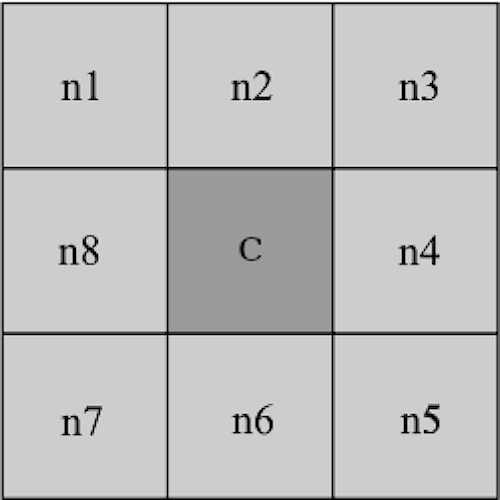
\includegraphics[width=0.3\linewidth]{imagenes/vecinosSharp.png}
  \caption[Vecinos de una celda en una grilla de ocupación.]{Vecinos de una celda en una grilla de ocupación.}
  \label{fig:vecinos}
\end{figure} 

Desde este punto se utilizará la función $ady$ como una función de adyacencia
genérica que puede ser tanto $ady_4$ como $ady_8$ a no ser que se indique lo
contrario.
Notar que la relación de adyacencia es simétrica por lo que $c_1 \in ady(c_2)
\Leftrightarrow c_2 \in ady(c_1)$.
% This map is obtained from the occupancy probability grid by a simple clipping operation with a threshold of 0.5. The gray areas of the maximum-likelihood map correspond to cells that have not been sensed by the robot.

\subsection{Componentes conexas} \label{subsec:CompComp}
Una descomposición en componentes conexas de un conjunto de
celdas $C \subseteq \mli{CG}$ es un conjunto $CC\in P(C)$ compuesto por $N$ conjuntos $C_i$ con
$i\in[1,N]$ tales que:
\begin{itemize}
  \item $\bigcup_{i=1}^{N}C_i = C$ 
  \item Para todo $i,j \in [1,N]$ con $i\neq j$ se cumple que  $C_i\cap C_j = \emptyset$
  \item Para todo $i \in [1,N]$, para todo $c_1,c_2 \in C_i$ 
    se cumple que existe un camino compuesto de celdas en $C_i$ que llevan
    desde $c_1$ a $c_2$.
  \item No existen $i,j \in [1,N]$ con $i\neq j$ tales que existan $c_1 \in C_i$ y $c_2 \in C_j$ que cumplan con $c_1 \in ady(c_2)$ 
\end{itemize}

Un ejemplo de una descomposición en componentes conexas se muestra en la figura \ref{fig:fronterasCompCon}.

\begin{figure}[H]
  \centering
  \subfloat[Las celdas pertenecientes a $C$ se marcan con azul.]{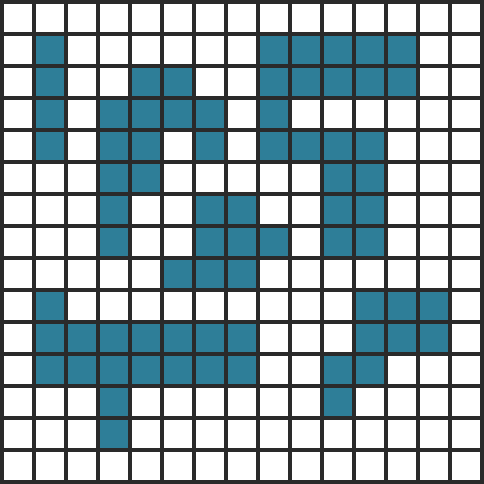
\includegraphics[clip=true, width=0.40\linewidth]{imagenes/compCon/a.png}}
  \qquad
  \subfloat[Cada componente conexa de $C$ se contornea con rojo.]{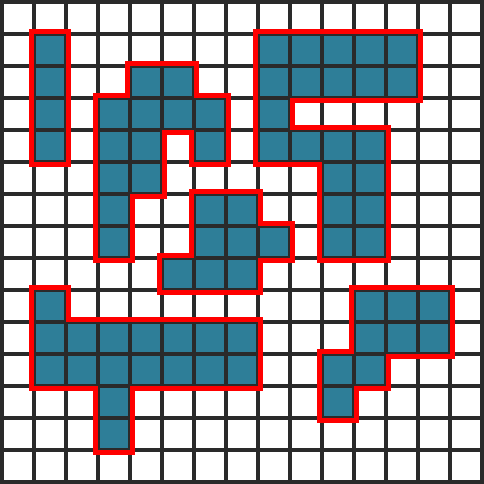
\includegraphics[clip=true, width=0.40\linewidth]{imagenes/compCon/b2.png}}

  \caption{Descomposición en componentes conexas.}\label{fig:descCompCon}
\end{figure}

Es posible obtener las componentes conexas de un conjunto cualquiera de
celdas $C$ con el algoritmo \ref{alg:compcon}.

\begin{algorithm}[H]
\SetAlgoLined
  \SetKwInOut{Input}{Entrada}
  \Input{$C$}
  $restantes := C$ \\
  $CC := \emptyset$ \\
  $pila :=$ Pila vacía \\
  $i := 1$ \\
  \While{ $restantes \neq \emptyset$ } {
    % $C_i := \emptyset $ \\
    $c :=$ elemento arbitrario de $Restantes$ \\

    % \tcp{DFS desde $c$ agregando las celdas visitadas a la componente conexa $C_i$}

    % $C_i :=  C_i \cup \{c\}$ \\
    $C_i :=  \{c\}$ \\
    $restantes := restantes - \{c\}$ \\
    $pila.apilar(c)$ \\
    \While { $\neg pila.vacia()$ } {
      $c := pila.desapilar()$ \\
      \ForEach{ $cA \in ady(c)$ } {
        \If{ $cA \in restantes$ } {
          $C_i :=  C_i \cup \{cA\}$ \\
          $restantes := restantes - \{cA\}$ \\
          $pila.apilar(cA)$ \\
        }
      }
    }
    $CC := CC \cup C_i$ \\
    $i := i + 1$ \\
  }
  \Return $CC$ 

  \caption{Descomposición en componentes conexas de $C$}
  \label{alg:compcon}
\end{algorithm}

El algoritmo se resume en elegir una celda $c\in C$ que no esté aún en una
componente conexa (línea 6) y aplicar un \emph{depth-first search} (DFS) desde
$c$, agregado todas las celdas recorridas a una misma componente conexa (líneas
7-19). Esto se repite hasta que todas las celdas pertenezcan a alguna
componente conexa (línea 5). Este algoritmo es análogo al que está presente en
\cite{hopcroft1973algorithm}.

% Este algoritmo es utilizado en la identificación de objetivos (sección
% \ref{sec:pc:idobj}) y para reconocer los segmentos del mapa (sección
% \ref{subsec:mapaTopGVDGrid})\todoremark{daría una pista sobre cuál sea la
% función del alg en el diseño de la solución.}.

\section{Identificación de objetivos}\label{sec:pc:idobj}
El problema de identificación de objetivos consiste en determinar puntos
del espacio a los cuales es conveniente enviar robots para recolectar nueva
información sobre el entorno explorado. Estos puntos son los llamados objetivos
de exploración (sección \ref{sec:exploracion}). 

\subsection{Fronteras}\label{subsec:todasFront}
En \cite{yamauchi1997frontier} se propone que los lugares que permiten
recolectar mayor cantidad de nueva información sobre el entorno son las
fronteras entre el espacio conocido y desconocido. Por lo tanto se establece que dichas
fronteras deben ser los objetivos de exploración.
Al utilizar una grilla de ocupación como mapa, las fronteras se definen como las
celdas cuyo estado asociado es $libre$ y son adyacentes a una celda cuyo estado
asociado es $desconocido$ (figura \ref{fig:fronteras}).
Por lo tanto según Yamauchi los objetivos de exploración serán las celdas
frontera $F$ según se definen en (\ref{eq:fronteras}).
\begin{equation} 
  F = \{ c \in \mli{CG} : e(c) = libre, \exists \mli{cA} \in ady(c), e(\mli{cA}) = desconocido  \}
  \label{eq:fronteras}
\end{equation}

En \cite{Amorin2019} se argumenta que tratar todas las celdas frontera como
objetivos de exploración diferentes podría ser computacionalmente prohibitivo.
Por lo tanto, para reducir el costo computacional, se reducen los objetivos de
exploración a las celdas frontera más representativas, las cuales se
denominan como fronteras significativas.

\subsection{Fronteras significativas basadas en K-Means}\label{subsec:simpKM}

En \cite{Amorin2019} se propone un método para obtener las fronteras
significativas que se basa en el algoritmo K-Means.

El método comienza descomponiendo al conjunto de celdas frontera $F$
en sus componentes conexas $\mli{FC}=\{F_1,F_2,...F_N\}$
(sección \ref{subsec:CompComp}), un ejemplo de este tipo de descomposición se
puede ver en la figura \ref{fig:fronterasCompCon}.

Luego se determinan las fronteras significativas $\mli{FS}_i$ de cada
componente conexa $F_i\in \mli{FC}$. Esto se hace agrupando las fronteras de
$F_i$ con el algoritmo K-Means \cite{macqueen1967some}, y determinando por cada
agrupación resultante, a una de las fronteras más cercanas de $F_i$ al
centroide de la agrupación como una frontera significativa. Un ejemplo de
las fronteras significativas $\mli{FS} = \bigcup_{i=1}^N \mli{FS_i}$ obtenidas
con este método se muestra en la figura \ref{fig:fronterasSig}.

El $k$ utilizado para ejecutar K-Means es el mínimo que logra que para toda
frontera $f\in F_i$ existe $\mli{fs} \in \mli{FS}_i$ tal que $d_{\mli{fs}}(f) \leq
rango$ siendo $rango$ el alcance de sensado de los robots. Es decir que %el conjunto de fronteras significativas $\mli{FS}_i \subseteq F_i$ cumple con que
cada frontera está dentro del rango del sensado desde alguna frontera
significativa, cuando esto se cumple se dice que $\mli{FS}_i$ cubre a $F_i$, o
que $\mli{FS}_i$ logra el cubrimiento. En la figura \ref{fig:fronterasSigCub} se
puede ver como las fronteras significativas obtenidas logran el cubrimiento.

% , ya que todos los centros de las fronteras de cada $F_i$ están
% contenidos en las circunferencias de radio $rango$ centradas en las fronteras
% significativas $\mli{FS}$.

Para encontrar el mínimo $k$ con las que se logra un $\mli{FS}_i$ que cubra a
$F_i$, se parte con $k=1$, y si el resultado no cubre a $F_i$ entonces se
incrementa $k$ en uno. Esto se repite hasta que el $\mli{FS}_i$ resultante
logre el cubrimiento.


\begin{figure}[H]
  \centering
  \subfloat[Se identifican las fronteras, indicadas con amarillo.]{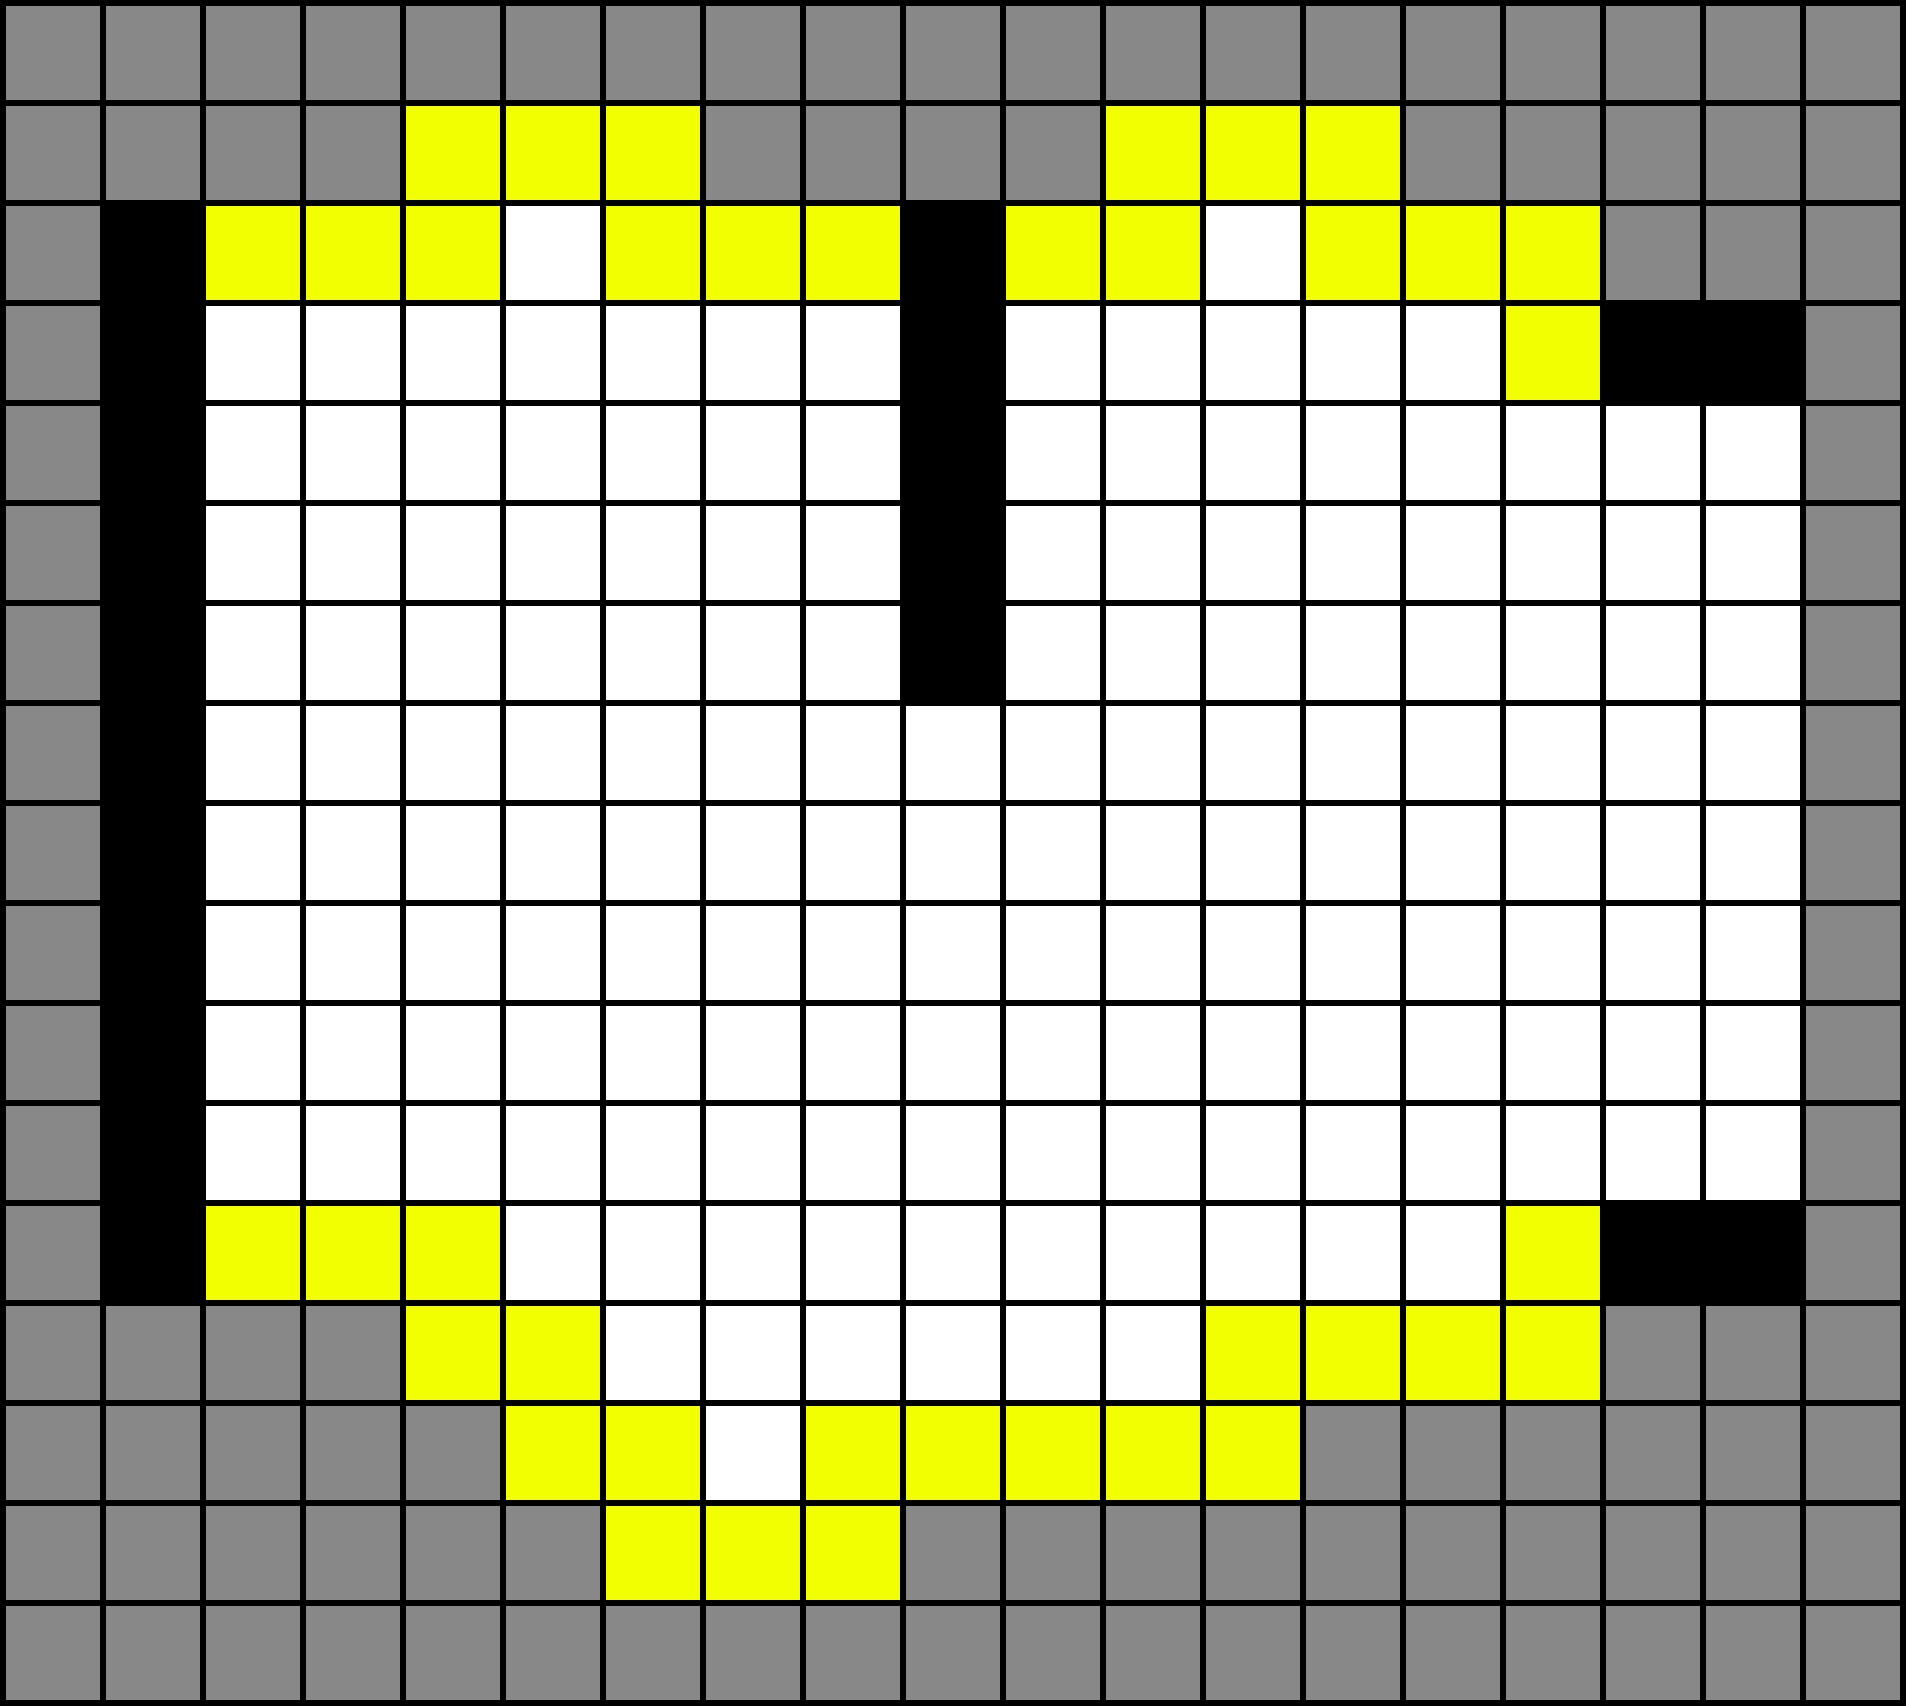
\includegraphics[clip=true, width=0.40\linewidth]{imagenes/fronterasSig/a.png}\label{fig:fronteras}}
  \qquad
  \subfloat[Descomposición de las fronteras en componentes conexas, cada componente conexa se indica con un color distinto.]{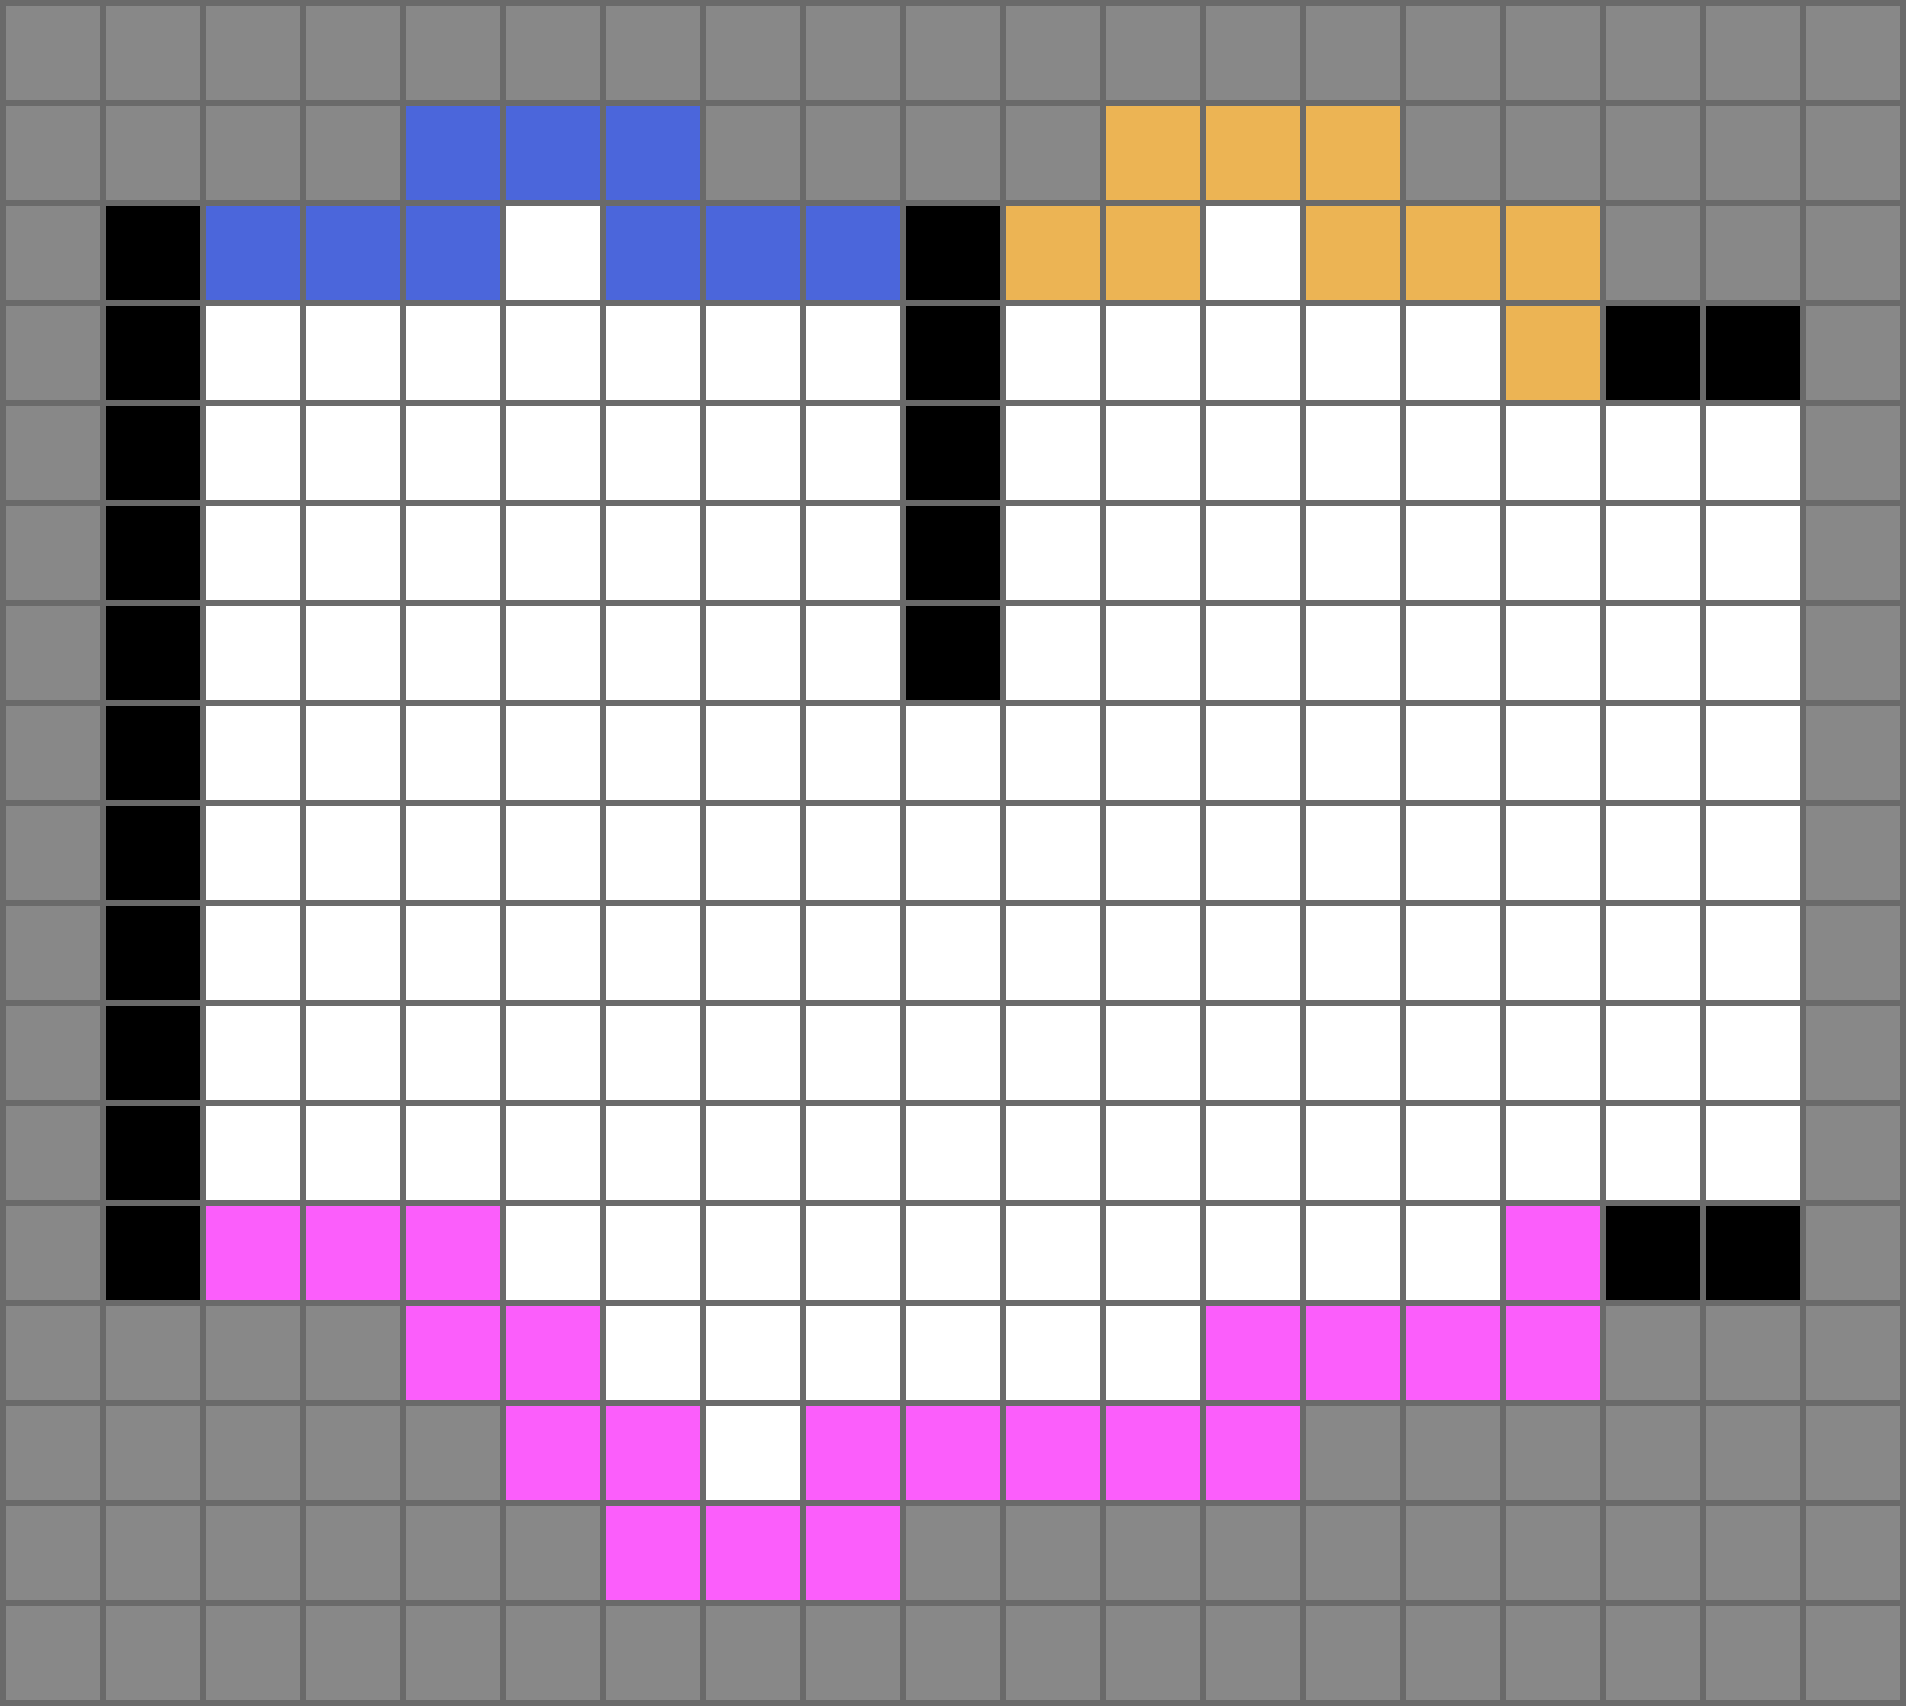
\includegraphics[clip=true, width=0.40\linewidth]{imagenes/fronterasSig/b.png}\label{fig:fronterasCompCon}}
  \qquad
  \subfloat[Fronteras significativas (indicadas con verde) de cada componente conexa.]{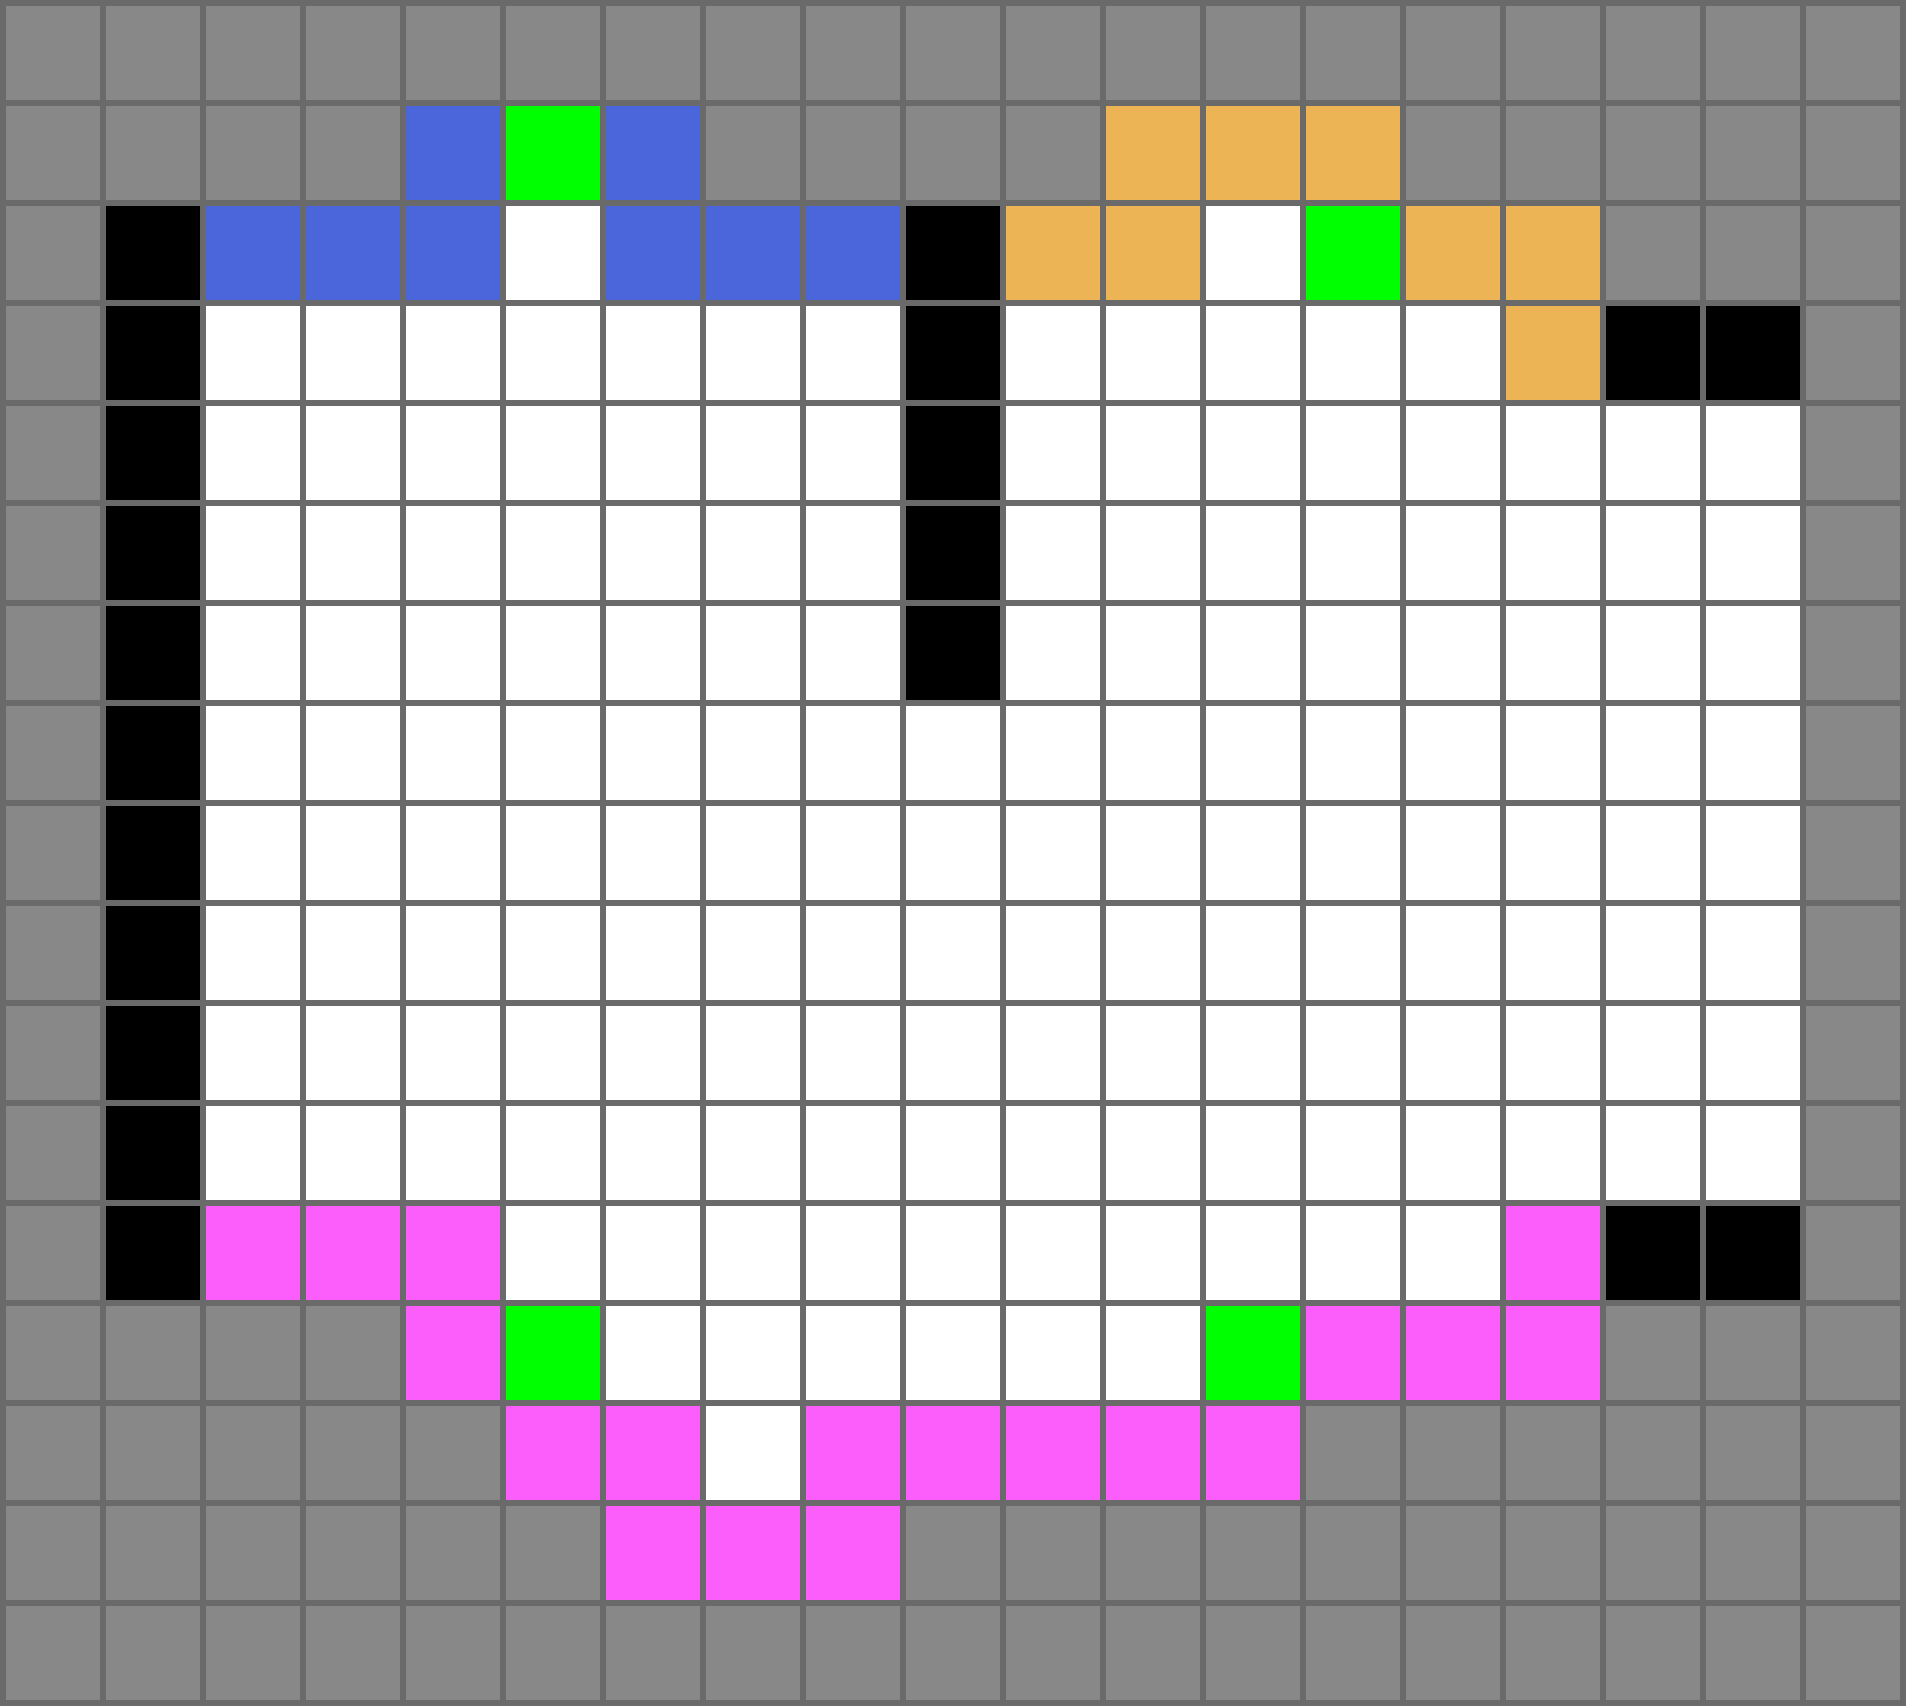
\includegraphics[clip=true, width=0.40\linewidth]{imagenes/fronterasSig/c.png}\label{fig:fronterasSig}}
  \qquad
  \subfloat[Se logra el cubrimiento.]{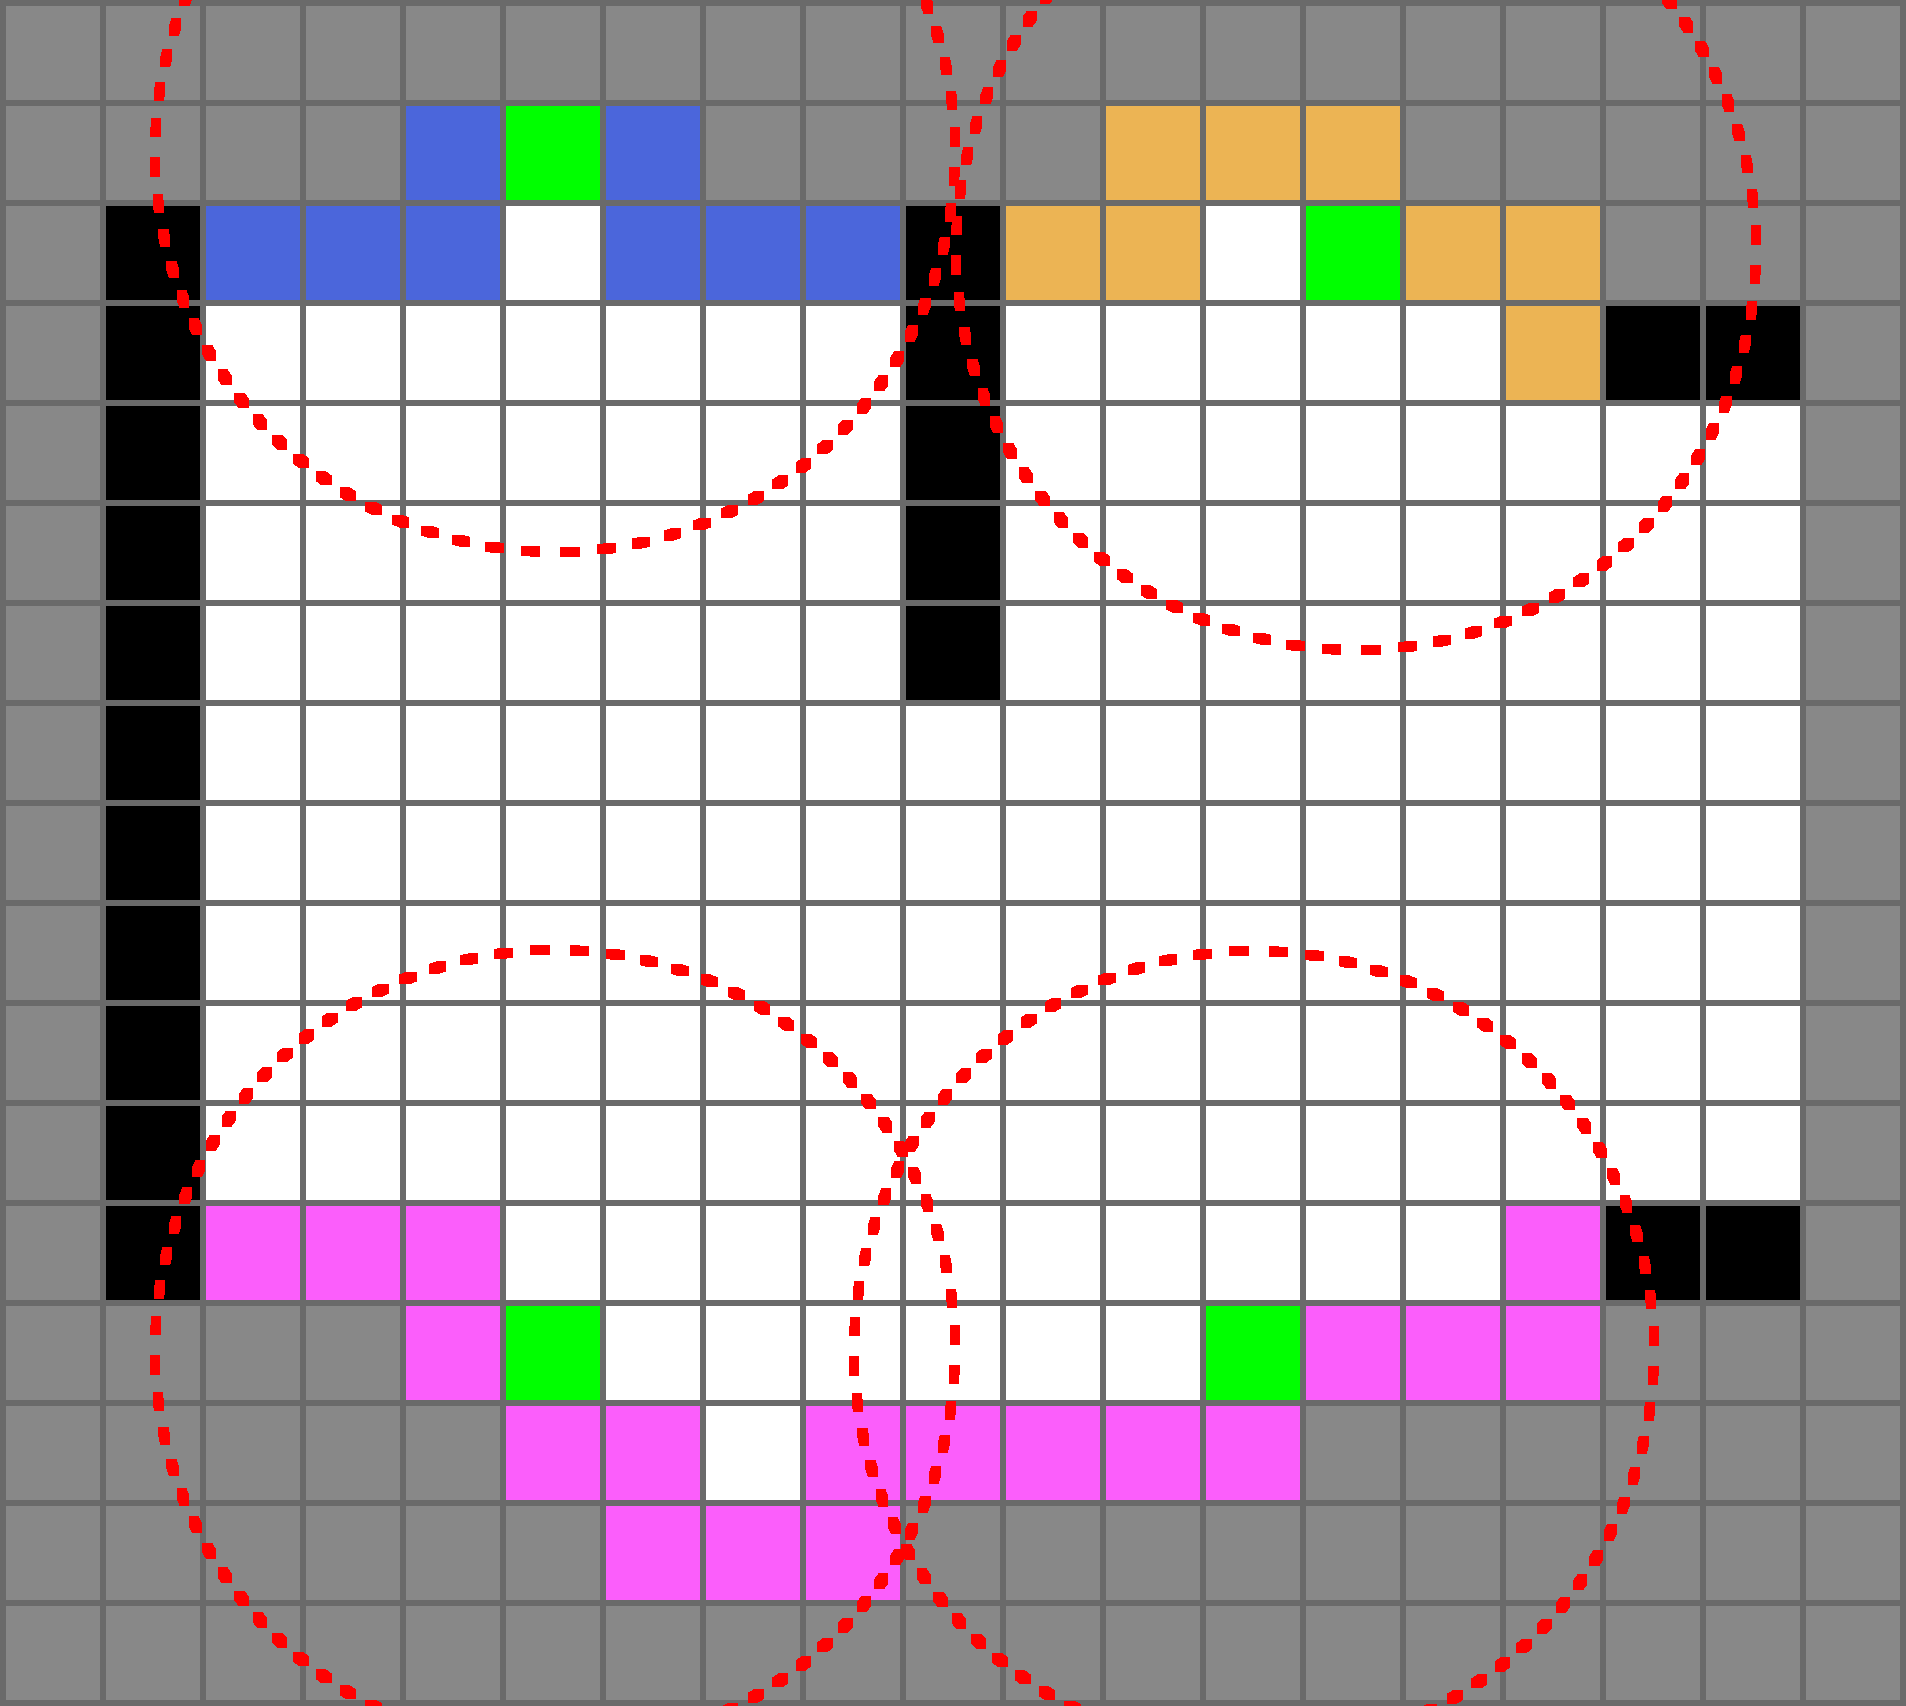
\includegraphics[clip=true, width=0.40\linewidth]{imagenes/fronterasSig/d.png}\label{fig:fronterasSigCub}}
  

  \caption[Proceso de obtención de fronteras significativas basado en K-Means.]{Proceso de
    obtención de fronteras significativas basado en K-Means. Las circunferencias rojas
    centradas en las fronteras significativas tienen un radio de $4\ lados\ de\ celda$ indicando su cubrimiento
    al usar sensores de rango equivalente. Basado en figuras de \cite{Amorin2019}.}\label{fig:ejemploFrontSig}
  % \caption[Proceso de obtención de fronteras significativas según K-Means.]{Proceso de obtención de fronteras significativas según K-Means. Cada figura corresponde a un mismo entorno parcialmente explorado, representado con una grilla, donde las celdas blancas son libres, las negras ocupadas, y para las grises se desconoce su estado. Basada en figuras de \cite{Amorin2019}.}\label{fig:ejemploFrontSig}
\end{figure}
% indicando su cubrimiento con un sensor de rango equivalente
% al usar un sensor de rango equivalente
% \todoremark[inline]{1: Lo cambie por basado en para ser consistente. 2: cambie largo de celda por lado de celda, quedo? | fig3.5: ... fronteras utilizando K-Means.? otra, ... tienen radio=4 celdas, indicando el cubrimiento de un sensor de rango equivalente. ?}

% En la seccion anterior se presento un método que soluciona el siguiente
% problema. Dado un conjunto de  la descomposición en componentes conexas de
% $F$, $\mli{FC}=\{F_1,F_2,...F_N\}$ se obteniene como salida el conjunto
% $\mli{FS} = \bigcup_{i=1}^N \mli{FS_i}$ que cumple con la restriccion de que
% para todo $i \in [1,N]$ $\mli{FS}_i$ cubre a $F_i$.

El problema descrito hasta el momento se resume en, dado un conjunto de
fronteras $F$, obtener un conjunto de fronteras significativas $\mli{FS}$ que
cumplen con la restricción de que $\mli{FS}$ cubre a $F$. Recordando que el
propósito de usar $\mli{FS}$ como objetivos de exploración en lugar de usar $F$
es reducir los objetivos de exploración, entonces es natural pensar que la
soluciones óptimas reducen al mínimo el $\mli{FS}$ resultante, mientras
mantienen la restricción de cubrimiento.

% Analizando la restriccion de cubrimiento, se puede ver que un indicador de que
% una solucion es subóptima es que varias celdas $\mli{FS}$ se concentren,
% solapandose las circunferencias de radio $rango$ centradas en ellas. Por
% ejemplo 

Dado esto es posible ver que en el ejemplo presentado en la figura
\ref{fig:ejemploFSKMMal} el resultado obtenido por el método presentado en esta
sección no es óptimo ya que existen fronteras significativas innecesarias para
el cubrimiento. 

\begin{figure}[H]
  \centering
  \subfloat[Fronteras significativas obtenidas según el método basado en K-Means.]{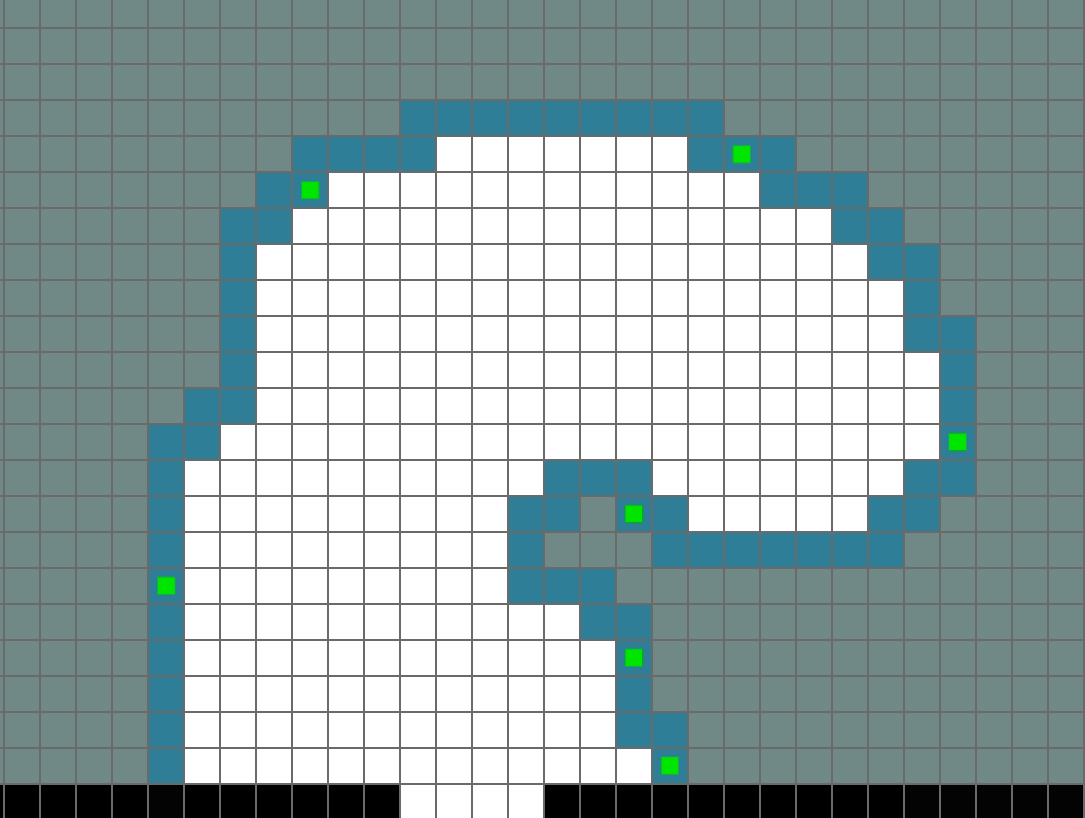
\includegraphics[clip=true, width=0.40\linewidth]{imagenes/fronterasigKMMal/caso1/a_sin_circ.png}}
  \qquad
  \subfloat[Dos de las fronteras significativas de la parte inferior derecha de (a) no son necesarias para lograr el cubrimiento.]{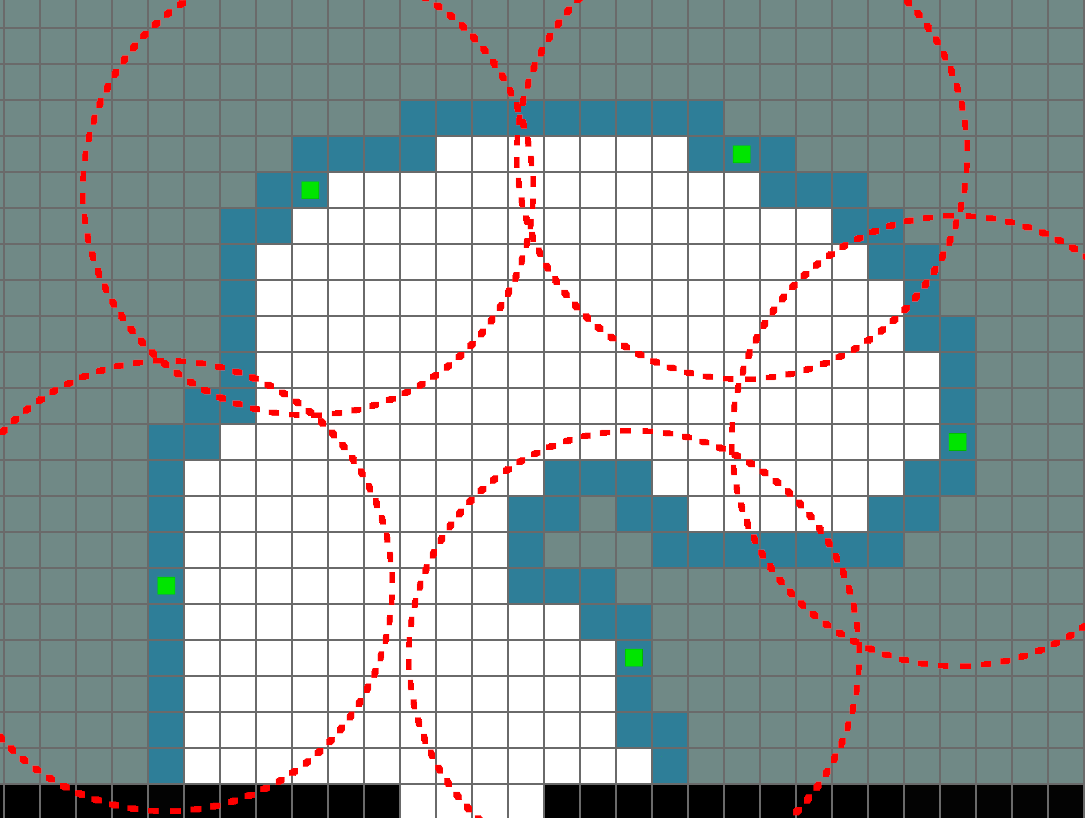
\includegraphics[clip=true, width=0.40\linewidth]{imagenes/fronterasigKMMal/caso1/b.png}}

  \caption[Resultado subóptimo del método de obtención de fronteras significativas basado en K-Means.]{Resultado subóptimo del método de obtención de fronteras significativas basado en K-Means. Las fronteras de $F_i$ se marcan con azul. Las fronteras significativas se indican con verde y las
    circunferencias rojas centradas en estas tienen un radio de $4\ lados\ de\ celda$ indicando su cubrimiento
    al usar sensores de rango equivalente.}\label{fig:ejemploFSKMMal}
\end{figure}
% \footnotetext{Podria indicar el bag y el }
%al aplicarse la simplificación 
Resultados subóptimos similares se experimentan de forma consistente sobre
componentes conexas de fronteras con forma serpenteante, asimétricas y lo suficientemente
extensas como para requerir más de 4 fronteras significativas para su
cubrimiento. 
%con un largo mayor a $rango*8$ 
% \todo[inline]{se entiende la idea del largo aplicada a esto? Creo que puede
% quedar claro mirando la foto pero tengo mis dudas. La idea en realidad sería
% decir que la solucion no es lo suficientemente simple, por ejemplo si con 1
% sola frontera sig ya se cubre todo entonces no va haber problema sin importar
% que tan serpenteante o asimetrica sea. Se me ocurre que puedo tratar la simpleza hablando por el largo puede
% quedar más claro o más oscuro, es decir por que 8? fue para poner un valor
% similar al de la foto que necesita 5 fronteras para cubrir }
Los resultados empeoran (mayor cantidad de fronteras significativas
innecesarias para el cubrimiento) a medida que las componentes conexas de
fronteras son más extensas y sus curvas son más pronunciadas.

% (comentarlos, distribuciones desparejas, acumulacion, no
% equidistantes) 

% Una explicacion posible a este comportamiento es que la distibucion de centroides en K-Means 

% Algo que se repite en estas situaciones es que suele haber zonas, en donde las
% fornteras significativas se acumulan, y zonas en las que estan muy dispersas
% (casi a $rango$ de distancia una de la otra, el maximo). Esto lleva a pensar que K-Means se tiende a ubicar concentrar los centroides en una zona,
% \todoerror[inline]{Creo que no se me entendió. A lo que me quiero referir acá es a que K-Means (no el método de simplificación entero, si no el algoritmo) no esta generando resultados pensando en cumplan la restricción de cubrimiento, si no que esto se comprueba luego (algo así como una fuerza bruta en un espacio de búsqueda muy reducido). El basado en cubrimiento lo soluciona porque su resultado por construcción cumple con la restricción de cubrimiento. Lo de que los resultados no pertenecen es el punto (ii) y el porque se explica antes | no está claro y es algo contradictorio el pto. tal vez señalar que k-means opera minimizando el error cuadrático medio de las distancias de las celdas a los centroides para conformar los clusters. esa operativa lleva a que los centroides no pertenezcan necesariamente al conjunto de celdas y también hace que aumentando el k se corrija ese aspecto.}
Esto se presume que se debe principalmente a dos factores relacionados a
K-Means: (i) K-Means no considera la restricción de cubrimiento para generar
sus resultados, sino que la restricción se fuerza obteniendo a través de prueba
y error al mínimo $k$ con el que las fronteras significativas resultantes
logran el cubrimiento. (ii) Los centroides resultantes de K-Means no son
necesariamente fronteras y deben ser traducidos a fronteras posteriormente.

% Esto se presume que se debe principalmente a dos factores relacionados a
% K-Means. (i) K-Means no considera la restricción de cubrimiento para generar
% sus resultados, sino que la restricción se fuerza ejecutando K-Means con el
% mínimo $k$ (obtenido con prueba y error) según el cual las fronteras
% significativas resultantes logran el cubrimiento. (ii) Los centroides
% resultantes de K-Means no son necesariamente fronteras y deben ser traducidos a
% fronteras posteriormente.



% \todo{Hay una arbitrariedad asociada a k-means tambien lo cual puede ser criticado tambien, aunque deberia estudiar mejor el tema, quizas no criticarlo aca pero destacar que el otro método es menos opaco en como elige las front sig}
% Esto es la clase de pe la idea de obtener fornteras significativas es reducir el número
% de objetivos de exploración,

% El método basado en K-Means aunque funciona bien al aplicase en componentes conexas pequeñas, 

% El método descrito en la seccion resulta en un conjunto de fronteras
% significativas que cubren a las fronteras, el problema que se detecto
% experimentalmente es que en ciertos casos el resultado  la discribucion de las
% fronteras significativas es mala, se concentran mucho en ciertas porciones y se alejan 

\subsection{Fronteras significativas basadas en cubrimiento}\label{subsec:MiSimp}
En esta sección se detalla un método de obtención de fronteras significativas novedoso,
que fue diseñado considerando los dos factores problemáticos relacionados al
método de obtención de fronteras significativas basado en K-Means, comentados
al final de la sección anterior. El factor (i) se toma en cuenta basando el
nuevo método en el concepto del cubrimiento, y el factor (ii) directamente
generado fronteras como resultado.

 % y su optimización
El método de obtención de fronteras significativas que se describe en esta sección, al igual que el
descrito en la sección anterior, comienza descomponiendo las fronteras $F$ en
sus componentes conexas $\mli{FC}=\{F_1,F_2,...F_N\}$, para luego obtener las
fronteras significativas $\mli{FS}_i$ de cada componente $F_i$. Siendo
$\mli{FS} = \bigcup^N_{i=1} \mli{FS}_i$ el conjunto total de fronteras
significativas. La principal diferencia radica en el proceso a través del cual
se obtienen las fronteras significativas $\mli{FS}_i$ de un componente $F_i$, que
se indica en el algoritmo \ref{alg:IdObjGeo}.

\begin{algorithm}[H]
\SetAlgoLined
  \SetKwInOut{Input}{Entrada}
  \Input{$F_i$}

  $\mli{FS}_i := \emptyset$\\
  $\mli{UF} := F_i$ \\

  $\mli{FP} :=$ Cola vacía \\
  \ForEach { $\mli{fp} \in \{f \in F_i : \exists \mli{c} \in ady(f), e(\mli{c}) = ocupado\}$} {
    $\mli{FP}.encolar(\mli{fp})$\\
  }
  \If{$\mli{FP}.vacia()$}{
    $\mli{FP}.encolar($elemento arbitrario de $F_i)$
  }
  \While{$\mli{UF} \neq \emptyset$ } {
    $\mli{fp} := \mli{FP}.desencolar()$\\
    \If{ $\mli{fp} \in \mli{UF}$}{
      $dCen := max \{ d_{\mli{fp}}(\mli{\mli{uf} }) : \mli{uf} \in\mli{UF} \}/2$\\
      $radio := min \{dCen, rango\}$\\
      $\mli{FSC} :=\mli{UF} \cap \mathscr{C}(\mli{fp},radio)$\\
      $\mli{fs} := $elemento arbitrario de $\mli{FSC}$\\
      $\mli{FS_i} := \mli{FS_i} \cup \{\mli{fs}\}$\\

      $\mli{RC} := \{ \mli{uf} \in \mli{UF} : d_{\mli{fs}}(\mli{uf}) \leq rango\}$\\

      $\mli{UF} := \mli{UF} - \mli{RC}$\\

      \ForEach { $\mli{fp} \in \{ \mli{uf} \in \mli{UF} : \exists \mli{rc} \in \mli{RC}, \mli{rc} \in ady(\mli{uf})\}$}{
        $\mli{FP}.encolar(\mli{fp})$
      }
    }
  }
  \Return $\mli{FS}_i$ 

  \caption{obtención de fronteras significativas basada en cubrimiento}
  \label{alg:IdObjGeo}
\end{algorithm}

%Para obtener las fronteras significativas de $F_i$ las fronteras significativas determinadas $\mli{FS}_i$
% (siglas del inglés \emph{uncovered frontiers})

El algoritmo mantiene en el conjunto $\mli{UF}$ a las fronteras de $F_i$ que
resta cubrir, y en una cola FIFO llamada $\mli{FP}$ a las próximas fronteras a
cubrir. Se comienza estableciendo que no se tienen todavía fronteras
significativas (línea 1) y  que resta cubrir a todas las fronteras (línea 2).
Luego se inicializa $\mli{FP}$ encolando en cualquier orden a las celdas
frontera de $F_i$ que son adyacentes a celdas de estado ocupado, y de no
existir ninguna frontera en estas condiciones encolando una única frontera
arbitraria de $F_i$ (líneas 3-9). 

Luego el algoritmo se basa en elegir una frontera de $\mli{UF}$ como frontera
significativa $\mli{fs}$ (líneas 11-16), y posteriormente actualizar las
estructuras mantenidas en función de la nueva $\mli{fs}$ (líneas 17-23). Notar
que esto implica reducir el número de celdas en $\mli{UF}$ ya que como mínimo
$\mli{fs}$ se cubre a sí misma. Este proceso de elección y actualización se
repite hasta que no quedan más fronteras de $F_i$ por cubrir (línea 10),
y finalmente se devuelven las fronteras significativas $\mli{FS_i}$ resultantes
(línea 25).
 
Ahora se profundizará sobre los procesos de elección (líneas 11-16) y
actualización de estructuras (líneas 17-23).

% El proceso de elección de $\mli{fs}$ tiene como objetivo el asegurar que se
% cubra una frontera $\mli{fp}$ desencolada de $\mli{FP}$ que todavía
% no este cubierta. Esto se traduce a la restricción $d_{\mli{fp}}(\mli{fs})
% \leq rango$. Adicionalmente se tiene una heurística que establece que dado
% $dCen = max\{ d_{\mli{fp}}(\mli{f}) : f\in\mli{UF} \}/2$, las fronteras que
% estén a $min \{dCen, rango\}$ de distancia de $\mli{fp}$ serán las mejores
% candidatas a ser fronteras significativas. La heurística busca elegir a las
% fronteras significativas que queden en el centro del conjunto de celdas nuevas
% que van a cubrir de $\mli{UF}$. Con esto en cuenta se determina un conjunto de
% fronteras significativas candidatas $\mli{FSC}$ como el conjunto de celdas que
% pertenecen a $\mli{UF}$ y a la circunferencia discretizada de $radio = min
% \{dCen, rango\}$ centrada en $\mli{FP}$ denotada como
% $\mathscr{C}(\mli{fp},rango)$ (\ref{eq:cir}).

El proceso de elección de $\mli{fs}$ tiene como objetivo el asegurar que se
cubra una frontera $\mli{fp}$ desencolada de $\mli{FP}$ que todavía no esté
cubierta. Esto se traduce a la restricción $d_{\mli{fp}}(\mli{fs}) \leq rango$.
Adicionalmente como heurística, sea $dCen = max\{ d_{\mli{fp}}(\mli{\mli{uf}}) :
\mli{uf}\in\mli{UF} \}/2$ se agrega la restricción $d_{\mli{fp}}(\mli{fs}) \leq dCen$.
Dicha heurística busca que las fronteras significativas $\mli{fs}$ elegidas queden
centradas en conjunto de las celdas de $\mli{UF}$ que van a cubrir. Con ambas
restricciones en cuenta se determina el conjunto de fronteras significativas
candidatas $\mli{FSC}$ como el conjunto de celdas que pertenecen tanto a $\mli{UF}$, como 
a la circunferencia discretizada centrada en $\mli{fp}$ y de $radio = min
\{dCen, rango\}$, que se denota como $\mathscr{C}(\mli{fp},radio)$
(\ref{eq:cir}).
% \todo[inline]{este concepto capaz no queda claro. Es muy específico y
% explicarlo me paree que corta un poco la narrativa. Dado el conjunto
% $Cir=\{f\in F_i : d_{\mli{fp}}(f) \leq radio\}$ son los puntos de $Cir$ que
% tienen un adyacente fuera de $Cir$ }
\begin{equation} \label{eq:cir}
\begin{aligned}
&\mathscr{D}(\mli{fp},radio) = \{c\in\mli{CG} : d_{\mli{fp}}(c) \leq radio\}\\ 
&\mathscr{C}(\mli{fp},radio) = \{c\in\mathscr{D}(\mli{fp},radio) : \exists cA \in ady(c), cA \notin \mathscr{D}(\mli{fp},radio) \}
\end{aligned}
\end{equation}
Y finalmente para elegir una nueva frontera significativa $\mli{fs}$ se elige una
frontera de las candidatas $\mli{FSC}$, en esta propuesta de forma arbitraria.

Por otro lado el proceso de actualización comienza agregando $\mli{fs}$ a
$\mli{FS}_i$, y determinando el conjunto de fronteras de $\mli{UF}$ que son
cubiertas por $\mli{fs}$, al que se denomina como $\mli{RC}$ (siglas de recién
cubiertas). Luego las fronteras de $\mli{RC}$ se remueven de $\mli{UF}$, y por
último se encolan en $\mli{FP}$ las fronteras de $\mli{UF}$ que son adyacentes
a las de $\mli{RC}$.

% utilizan para
% determinar que celdas encolar a $\mli{FP}$, siendo las fronteras encoladas para
% .

% . El
% encolar nuevas fronteras en $\mli{FP}$ es necesario para que el criterio de
% elección propuesto funcione de forma correcta, 

Un ejemplo de ejecución para el caso presentado en la figura
\ref{fig:ejemploFSKMMal} se muestra en la figura \ref{fig:ejemploFSCub}. En el
apéndice \ref{EXE:sfbc} se muestra la misma ejecución con un mayor nivel de
detalle.

\begin{figure}[H]
  \centerfloat
  \subfloat[Incializacion de $\mli{FP}$, $\mli{UF}$ y $\mli{FS_i}$.]{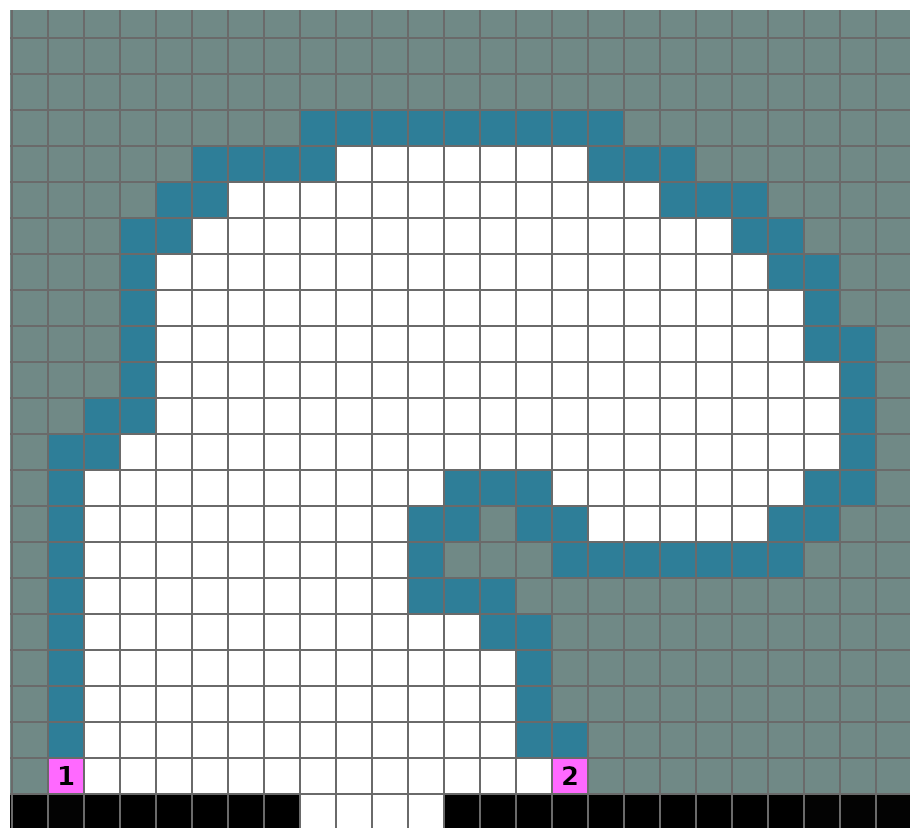
\includegraphics[clip=true, width=0.40\textwidth]{imagenes/ejemploSimpCub/a2.png}}
  \subfloat[Se elige un nuevo $\mli{fs}$ y se actualizan $\mli{UF}$, $\mli{FS_i}$ y $\mli{FP}$.]{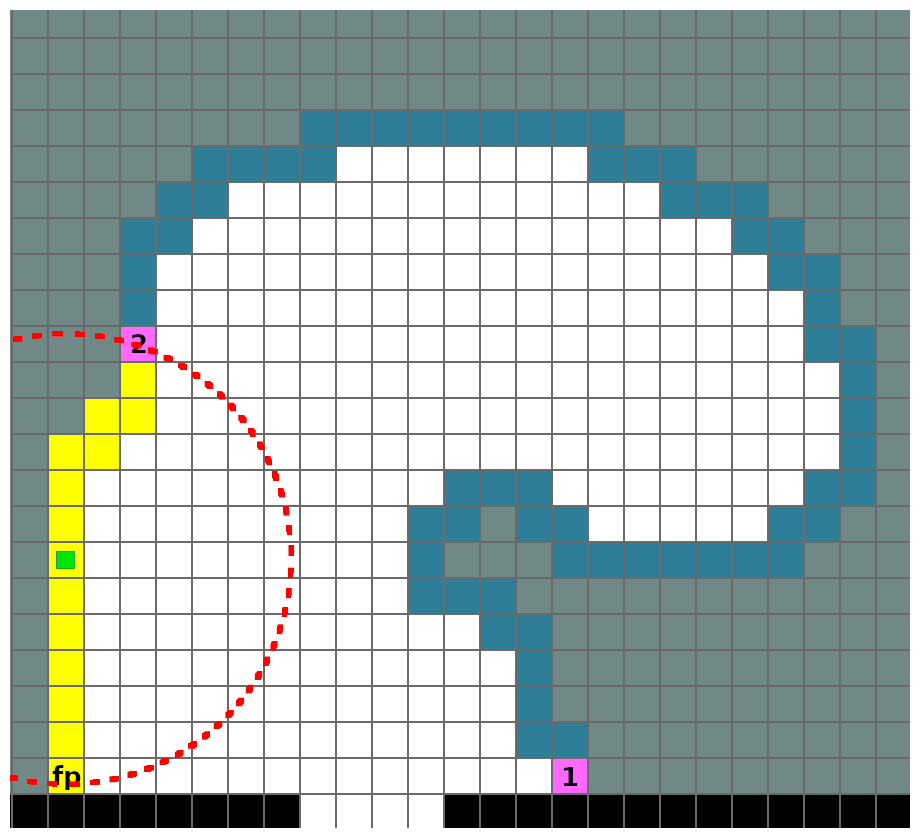
\includegraphics[clip=true, width=0.40\textwidth]{imagenes/ejemploSimpCub/b5.png}}
  \subfloat[Se elige un nuevo $\mli{fs}$ y se actualizan $\mli{UF}$, $\mli{FS_i}$ y $\mli{FP}$.]{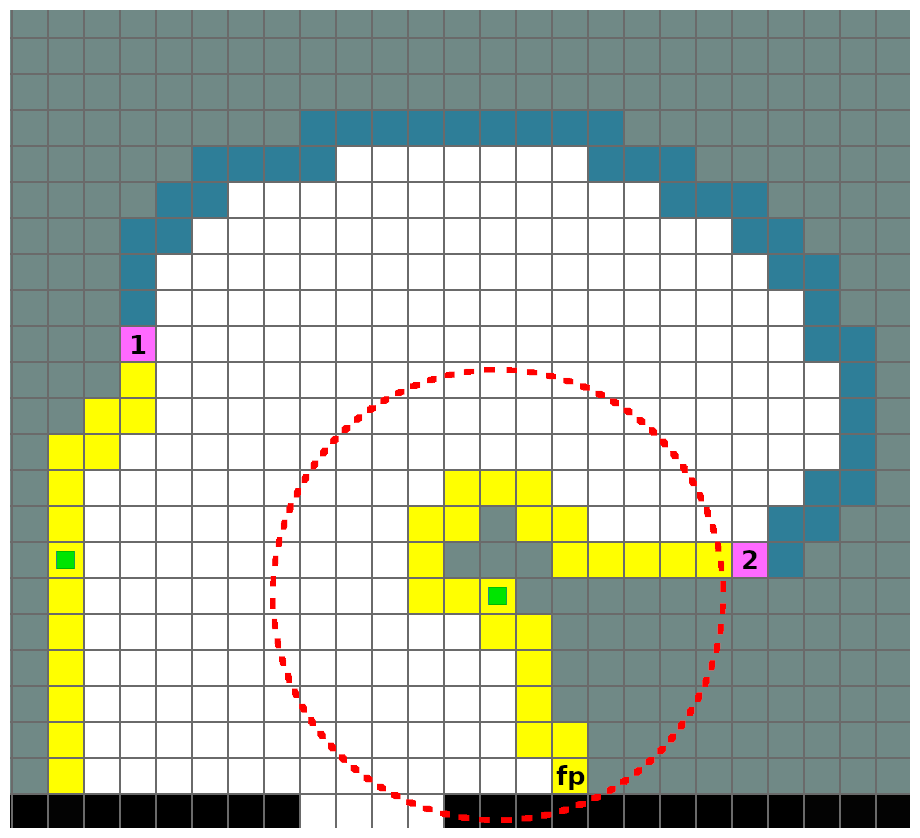
\includegraphics[clip=true, width=0.40\textwidth]{imagenes/ejemploSimpCub/c5.png}}

  \subfloat[Se elige un nuevo $\mli{fs}$ y se actualizan $\mli{UF}$, $\mli{FS_i}$ y $\mli{FP}$.]{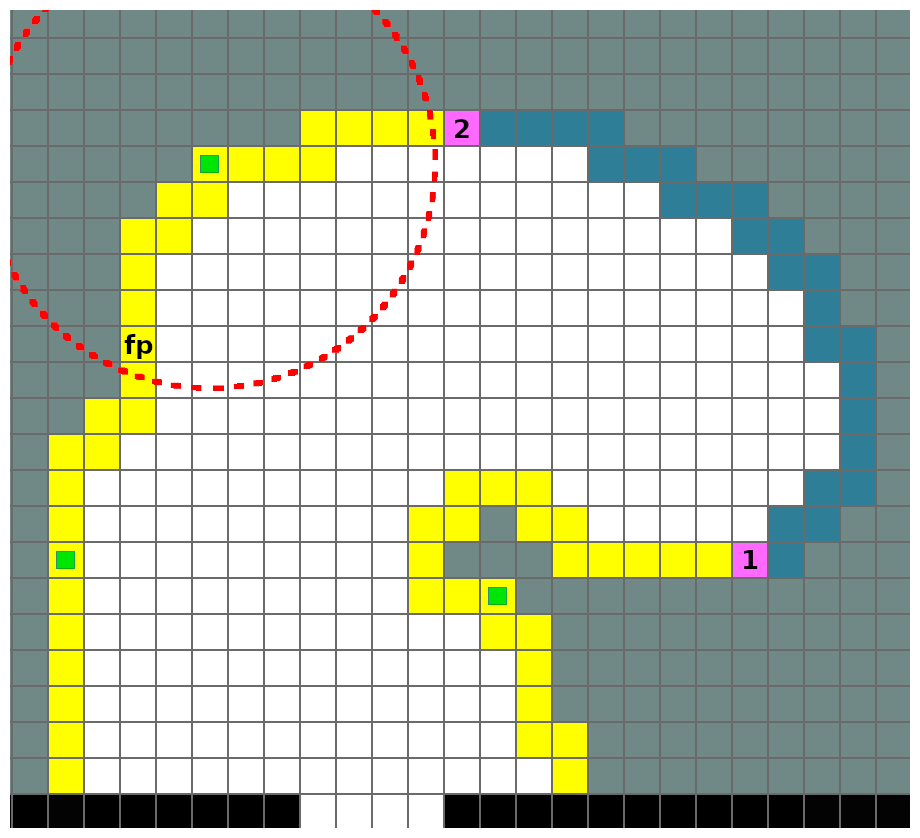
\includegraphics[clip=true, width=0.40\textwidth]{imagenes/ejemploSimpCub/d5.png}}
  \subfloat[Se elige un nuevo $\mli{fs}$ y se actualizan $\mli{UF}$, $\mli{FS_i}$ y $\mli{FP}$.]{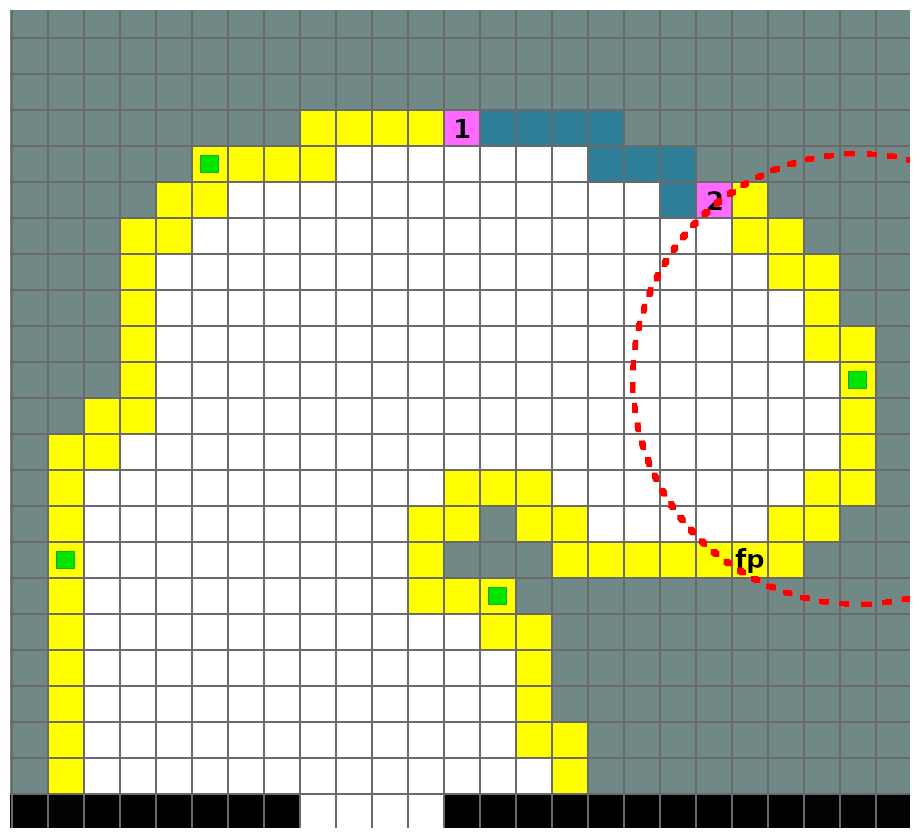
\includegraphics[clip=true, width=0.40\textwidth]{imagenes/ejemploSimpCub/e5.png}}
  \subfloat[Se elige un nuevo $\mli{fs}$ y se actualizan $\mli{UF}$, $\mli{FS_i}$ y $\mli{FP}$.]{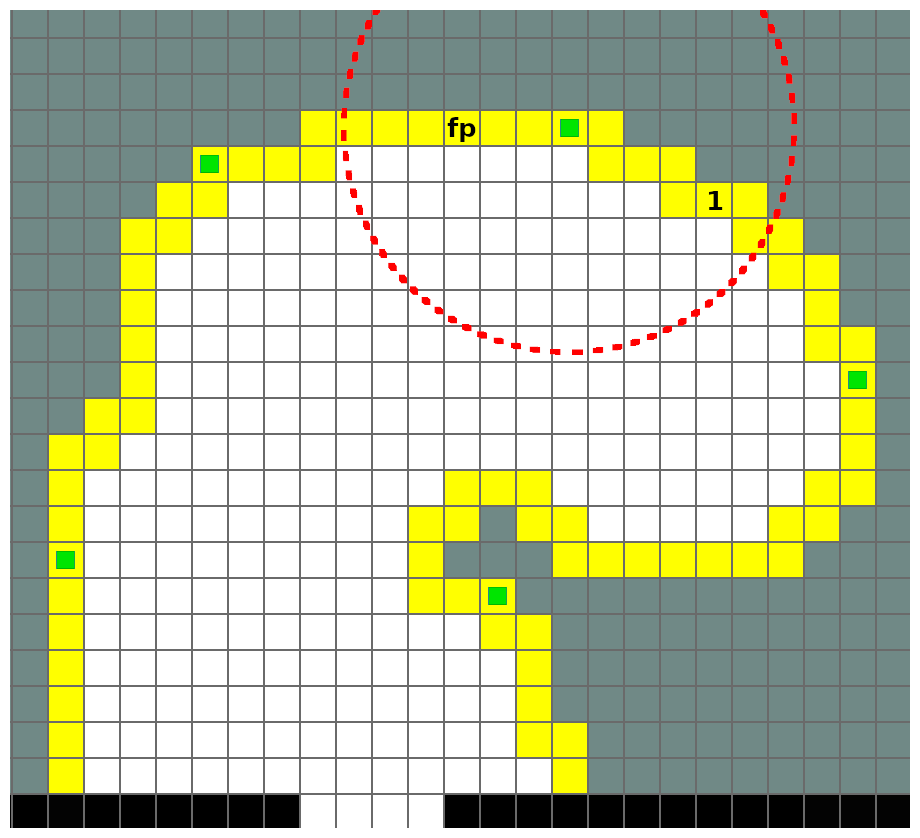
\includegraphics[clip=true, width=0.40\textwidth]{imagenes/ejemploSimpCub/f4.png}}
 \phantomcaption
\end{figure}
\addtocounter{figure}{-1} 

\begin{figure}[H]
  \centerfloat
  \setcounter{subfigure}{6}
  \subfloat[$\mli{UF}=\emptyset$ por lo que el algorimo finaliza.]{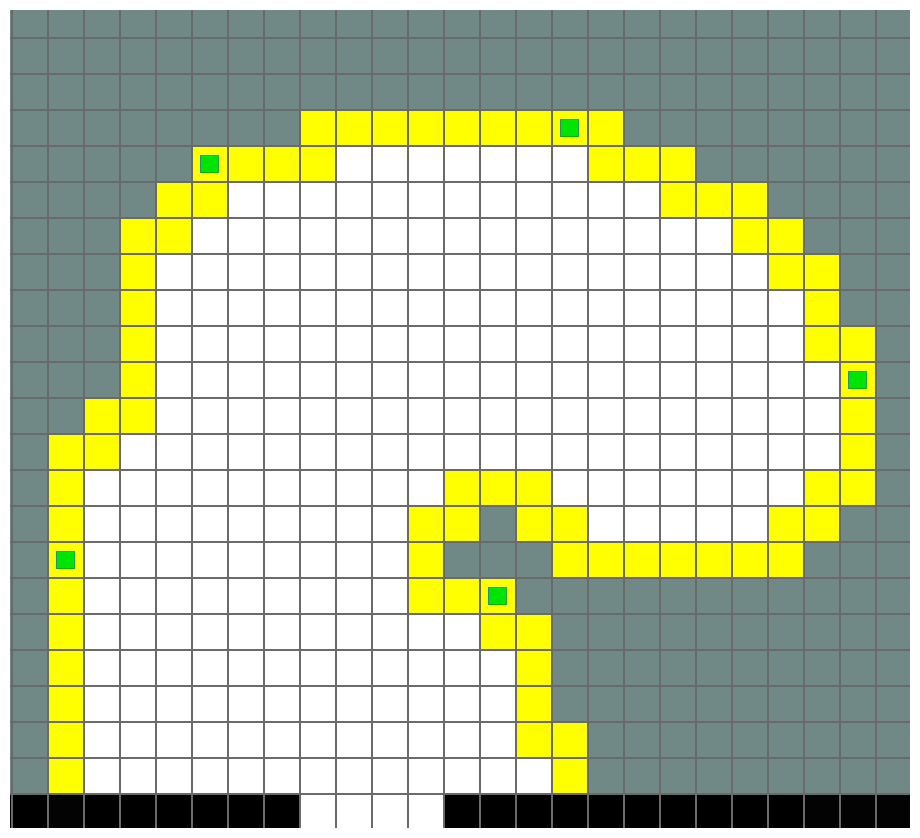
\includegraphics[clip=true, width=0.40\textwidth]{imagenes/ejemploSimpCub/zfinal1.png}}
  \subfloat[Se logra el cubrimiento.]{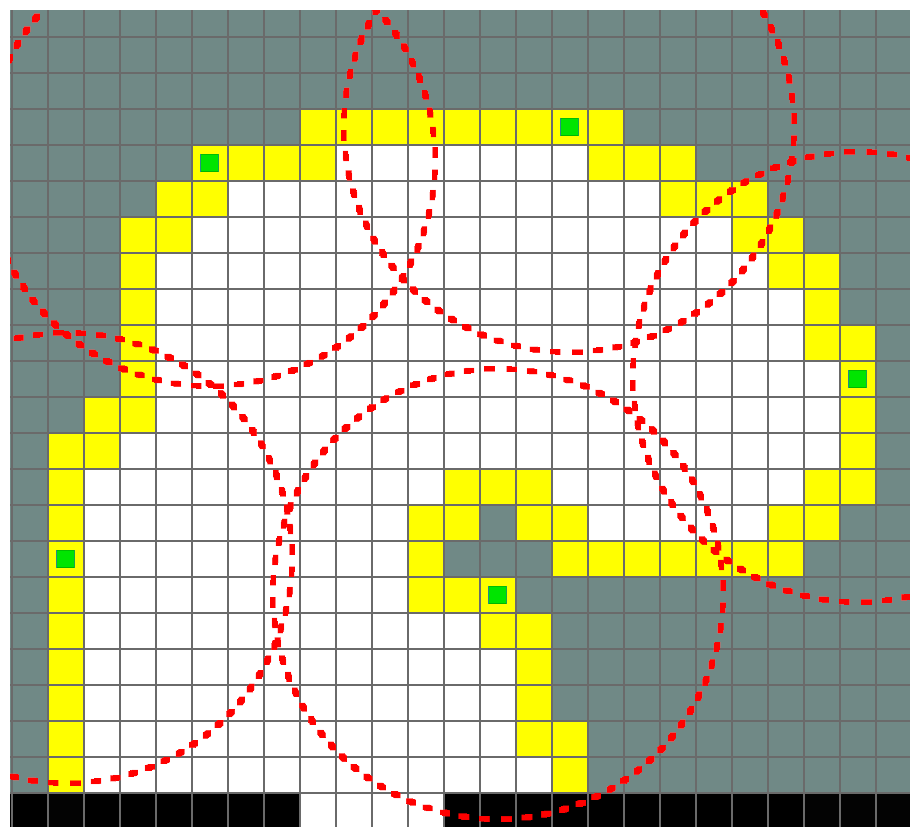
\includegraphics[clip=true, width=0.40\textwidth]{imagenes/ejemploSimpCub/zfinal2.png}}

  \caption[Proceso de obtención de fronteras significativas basado en cubrimiento.]{Proceso
    de obtención de fronteras significativas basado en cubrimiento. Las fronteras de
    $F_i$ se indican con azul si pertenecen a $\mli{UF}$ y con amarillo de lo
    contrario. Con magenta se indican las celdas en $\mli{FP}$ siendo la
    numeración su orden en la cola, y $\mli{fp}$ la última desencolada. Las fronteras significativas se indican con
    verde y las circunferencias rojas centradas en estas tienen un radio de $4\
  lados\ de\ celda$ indicando su cubrimiento
    al usar sensores de rango equivalente.}\label{fig:ejemploFSCub}
\end{figure}

\section{Asignación de objetivos}\label{sec:asigTar}

Cuando un robot se encuentra ocioso este le solicita a la central que le asigne
un nuevo objetivo de exploración, esto desencadena el proceso de asignación de
objetivos que se describe a lo largo de esta sección.

La asignación de objetivos se basa en la estrategia de coordinación presentada
en \ref{subsec:wurmCoord}, que sostiene que es conveniente que los robots se
asignen a los objetivos maximizando la distribución de los robots
sobre los segmentos (habitaciones y corredores) que componen un entorno
estructurado.
% , que
% se corresponden las regiones de un mapa topológico (sección
% \ref{subsec:mapas}).

La asignación de objetivos consiste una subasta donde lo subastado son los
objetivos de exploración, el subastador es la estación central y los postores
son los robots. La subasta se puede separar en tres partes, \emph{obtención de
  información}, \emph{valuación} y \emph{resolución}. La \emph{obtención de
información} es la etapa inicial donde la central obtiene la información necesaria
para llevar adelante la subasta, por ejemplo los objetivos de exploración. La
\emph{valuación} abarca la distribución de la información obtenida desde la
central hacia los robots, la valuación que cada robot hace para cada objetivo
recibido y el posterior envió de las valuaciones desde los robots hacia la
central. La \emph{resolución} se lleva a cabo en la central y comprende la
recepción de las valuaciones, la determinación de que objetivo asignar a cada a
robot y la notificación a cada robot del objetivo que le fue asignado.

% según la valuaciones y
% los segmentos a los cuales pertenece cada objetivo

% Con respecto a la separación del problema de asignación de objetivos mencionada
% en la sección \ref{sec:exploracion}, la parte de identificación de objetivos
% esta incluida en la \emph{obtención de información}, y la parte de
% distribución de objetivos se corresponde con el resto de lo que se describe
% en esta sección.

\subsection{Obtención de información}\label{subsec:obtInfo}
%, esto desencadena una nueva subasta de no encontrarse una en curso.
% Notar que si existe una subasta en curso el robot va recibir un objetivo cuando
% esta termine, por lo que puede no ser necesario iniciar otra.
Como se menciono anteriormente cuando un robot ocioso solicita un objetivo a la
central se da comienzo a una nueva subasta. La etapa de \emph{obtención
información} es la primera etapa de la subasta. La información que se obtiene
en esta etapa son los objetivos de exploración, los segmentos del entorno
explorado y un GVD.
% que con el motivo
% de identificar en que segmento se encuentra cada objetivo de exploración, para
% posteriormente poder distribuir a los robots sobre estos. 

La identificación de objetivos se lleva a cabo con el método descrito en la
sección \ref{subsec:MiSimp}.

Los segmentos se obtienen aplicando una técnica que se basa en la propuesta de
\cite{Thrun1998} explicada en la sección \ref{subsec:mapaTopGVD}. Detalles de
como esta técnica fue implementada se presentan en la sección
\ref{subsec:mapaTopGVDGrid}. 

El GVD requerido para determinar los segmentos se construye de forma
incremental con una variante del \emph{brushfire dinámico} que se comenta en la
sección \ref{sec:MiConstGVD}.
% de no de los cambios principales con
% respecto al trabajo original de \cite{wurm2008coordinated} es la forma en la
% cual se contruye el GVD. En el trabajo original se hace uso de un método de
% construccion no incremental, en este proyecto con el motivo de alcanzar una
% implementación eficiente para su uso en tiempo real (seccion
% \ref{subsec:constGVDInc})

\subsection{Valuación} \label{subsec:MiValSub}

Terminada la etapa obtención de información comienza la etapa de \emph{valuación} con la
central distribuyendo los objetivos y el GVD hacia los robots. 

Cuando un robot recibe dicha información este calcula dos valores para cada
objetivo, el largo de un camino hacia él y un costo asociado a la complejidad
de ese camino. Esto implica determinar un camino. En este proyecto los caminos
se componen de una secuencia de puntos en el espacio que comienza en la
posición del robot y termina en el objetivo. Los caminos se calculan de forma
distinta dependiendo de la clase de objetivo al que llevan, existiendo dos
clases, trivial y no trivial.

Los objetivos triviales se definen como los objetivos para los cuales el
segmento de recta que existe entre el robot y el objetivo no contiene
obstáculos, de lo contrario el objetivo es no trivial. Para determinar esto, se
discretiza el segmento de recta en celdas \cite{foleyphillips} y se comprueba
en la grilla de ocupación almacenada en el robot (que constituye el mapa
completo del entorno) si alguna de esas celdas tiene estado ocupado. 

Los caminos hacia los objetivos triviales se determinan como los puntos
ubicados en los extremos del segmento de recta que se encuentra libre de
obstáculos que existe entre el robot y el objetivo. Un ejemplo de un camino
trivial se muestra en la figura \ref{fig:caminoT}.

En el caso de los objetivos no triviales se hace uso del GVD recibido como
parte de la información de la subasta, aprovechando que este constituye un
\emph{roadmap} (sección \ref{subsec:mapacarr}). En este caso el proceso para
construir el camino se puede dividir en tres partes, cada una asociada a una de
las propiedades que caracterizan a un \emph{roadmap}: accesibilidad,
conectividad y capacidad de salida. La parte asociada a la accesibilidad
consiste en encontrar un camino desde el robot al GVD, lo cual se hace a través
de un \emph{breadth-first search} (BFS), comenzando en la celda asociada a la
posición del robot y deteniéndose apenas se visita una celda $c_1$
perteneciente al GVD. La parte que se relaciona a la capacidad de salida es
análoga a la parte asociada a la accesibilidad pero partiendo desde el objetivo
y llegando a una celda $c_2$ perteneciente al GVD. Por último en la parte
vinculada con la conectividad se determina un camino sobre las celdas
pertenecientes al GVD desde $c_1$ a $c_2$, y para esto se utiliza el algoritmo
$A^*$. Finalmente conectando los tres caminos se obtiene el camino completo. En
la figura \ref{fig:caminoNT} se presenta un ejemplo de un camino para un
objetivo no trivial.

\begin{figure}[H]
  \centerfloat

  \subfloat[Trivial.]{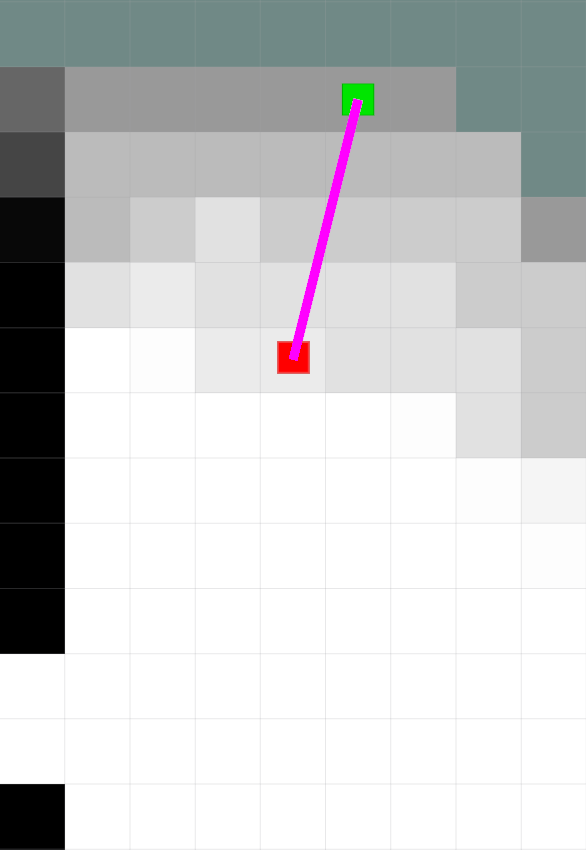
\includegraphics[clip=true, width=0.25\textwidth]{imagenes/camino/caminoTsinGVDRecortado.png}\label{fig:caminoT}}
  \qquad
  \subfloat[No trivial.]{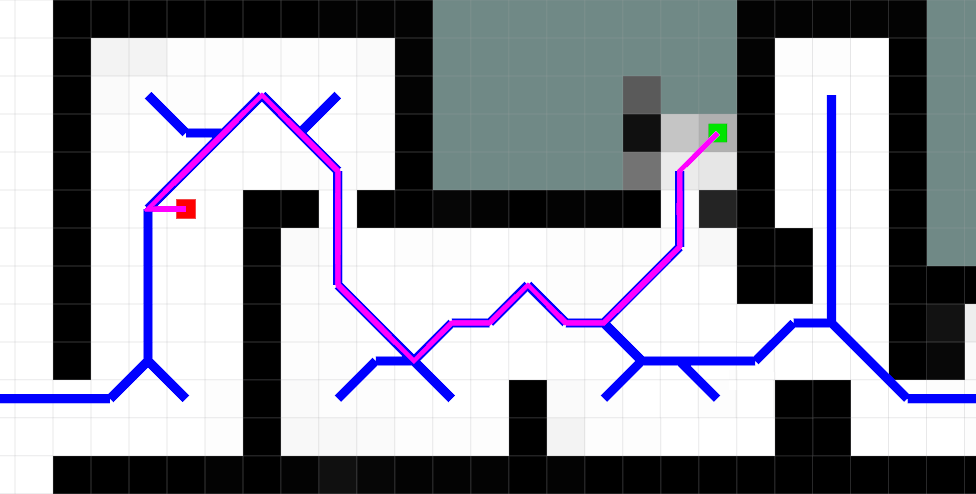
\includegraphics[clip=true, width=0.70\textwidth]{imagenes/camino/camino.png}\label{fig:caminoNT}}

  \caption[Camino.]{Caminos calculados desde la posición del robot indicada en
  rojo, hasta el objetivo indicado en verde. Los puntos del camino se conectan
entre sí con líneas magenta.}\label{fig:camino}

\end{figure}


Respecto al costo asociado a la complejidad, en el caso de objetivos triviales
este es proporcional al mínimo ángulo que el robot debe rotar para que su parte
delantera apunte hacia el objetivo. Y en el caso de objetivos no triviales es
igual al máximo costo asociado a la complejidad que fue asignado a un objetivo
trivial, esto se hace para diferenciar los objetivos triviales sin dejar
beneficiados a los objetivos no triviales. Este costo tiene el propósito de
incentivar que los robots continúen siendo asignados a los objetivos triviales que
tienen por delante, evitando rotaciones, a no ser que la diferencia en los largos de
los caminos lo amerite.

Una vez calculados los valores para cada objetivo estos se envían hacia la central
junto a la ubicación actual del robot, siendo toda esta información en su
conjunto considerada una valuación. %\todo{o mensaje de valuación, como quede mejor}

% Respecto al costo asociado a la complejidad, en el caso de objetivos triviales
% este corresponde a una estimación del tiempo que demora el robot en rotar de
% forma que su parte delantera apunte hacia el objetivo. Y en el caso de
% objetivos no triviales se utiliza el máximo costo asociado a la complejidad que
% fue asignado a un objetivo no trivial, esto se hace para diferenciar los
% objetivos triviales sin beneficiar a los objetivos no triviales. Este costo
% tiene el propósito de incentivar que los robots continúen siendo asignados a
% objetivos triviales que tienen por delante, evitando que roten a no ser que la
% diferencia de largos de los caminos lo amerite.


% De esta
% forma los objetivos triviales se valuan distinto según que tanto tiene que
% rotar el robot para llegar a ellos y los objetivos no triviales tendran un
% costo no mayor al del peor objetivo no trivial.

% como el conjunto de celdas que abarca, el proceso para construir el camino es
% se puede dividir en encontrar tres subcaminos cada uno relacionado a una de las
% tres propiedades de un roadmap: accesibilidad, conectividad y capacidad de
% salida. La accesibilidad consiste en encontrar un camino desde el robot al GVD,

% La valuacion abarca la distribuicion de los objetivos de exploración desde la
% central hacia los robots, la asignación de valores que cada robot debe hacer a
% cada objetivo y el posterior envio de estas valoraciones desde los robots hacia
% la central. 

\subsection{Resolución} \label{subsec:MiResSub}
La etapa de resolución comienza con la central recibiendo las valuaciones
realizadas por los robots. Al recibirse la primera valuación existe una ventana
de tiempo en que la central continuará recibiendo nuevas valuaciones.
Terminada esta ventana se ejecuta un algoritmo que asigna objetivos a los
robots. Y por último las asignaciones realizadas son comunicadas a los robots.
% La resolución es el proceso de asignar los objetivos La resolución contempla
% la recepción de las valoraciones por la central, la asignación de objetivos a

% robots según y la notificación del objetivo asignado a los robots. 
% de exploración a los
% robots. 
\subsubsection{Recepción de valuaciones}
Como se menciono anteriormente luego de recibida la primera valuación existe
una ventana de tiempo en la que la central continuará recibiendo nuevas
valuaciones.%, luego de la cual se da por concluida la recepción de valuaciones. 

El propósito de utilizar una ventana de tiempo es que en escenarios reales
existen razones por las cuales los robots pueden dejar de comunicarse, como por
ejemplo accidentes que causen problemas de hardware. Por lo tanto esperar
por las valuaciones de todos los robots puede resultar en una espera infinita que
deja inoperativa a toda la flota.


Dado que los problemas que cada robot debe resolver para generar su valuación
son similares entre sí, se asume que los tiempos que demoran en generarla también
son similares. Adicionalmente dichos tiempos tienden a aumentar a medida que el
entorno es explorado. Por lo tanto se optó por utilizar una ventana dinámica
cuya duración es calculada en función de la demora de la recepción de
valuaciones experimentada en la subasta anterior, buscando que la duración de la ventana sea suficiente para que todos
los robots que estén en condiciones de enviar sus valuaciones tengan el
tiempo necesario para hacerlo.

Notar que una vez que se reciben las valuaciones de todos los robots
en funcionamiento es innecesario continuar esperando, por lo tanto de recibirse
dichas valuaciones la ventana es terminada prematuramente, evitando esperas
innecesarias.

Sea $\mli{\Delta r}_{i-1}$ el tiempo que paso en la subasta $i-1$ desde la recepción de la
primera valuación hasta que se da por terminada la recepción valuaciones,  %comienzo de la ejecución del algoritmo de asignación que marca el final de la recepcion
la duración $\mli{Vr}_i$ de la ventana en la subasta $i$ se define según
(\ref{eq:ventanaVals}).

\begin{equation} 
  \mli{Vr}_i = 
  \left \{ 
    \begin{aligned}
      0.5s                            \ \ \ \ \ \ \ \ & si\ i = 0\\ 
      max(0.5s + 2\mli{\Delta r}_{i-1}, \mli{Vr}_{i-1}) \ \ \ \ \ \ \ \ & si\ i > 0
    \end{aligned}
  \right .
  \label{eq:ventanaVals}
\end{equation}

El valor de la duración $\mli{Vr}_i$ resulta de asumir que el tiempo que se demora en
recibir las valuaciones no aumenta más del doble de una subasta a la siguiente.
Adicionalmente dando un margen de error de 0.5 segundos, especialmente
útil cuando $\mli{\Delta r}_{i-1}$ es muy pequeño. 

% Lo asumido se corresponde con lo ocurre en
% las pruebas realizadas.

% por lo que sería contraproducente no esperar por la valoración de
% algún robot ya que dicha espera es mínima en comparación con lo que un robot
% debe esperar en caso de no ser considerado para la resolución.

% Para cumplir con el propósito propuesto se podría decir que la ventana sea de
% un tamaño muy grande o infinita, lo cual en un entorno simulado como el que se
% basa este trabajo no generaría problemas ya que los robots siempre pueden


% y como estas se guardan al recibirse
\subsubsection{Algoritmo de asignación de objetivos}
% Según lo explicado en la sección anterior
% ($-10$ en al implementación)

Cuando la central recibe una valuación de un robot $r_i$, esta se encarga de
procesar la información contenida en la valuación de forma de obtener un único
costo $c_{i,j}$ para cada objetivo $o_j$. Dado un objetivo $o_j$ la valuación
del robot $r_i$ contiene el largo $\mli{cl}_{i,j}$ del camino de $r_i$ a $o_j$,
y el costo $\mli{cc}_{i,j}$ asociado a la complejidad de dicho camino.
Adicionalmente contiene la posición de $r_i$ a través de la cual se determina
un descuento $\mli{ds}_{i,j}$ que toma un valor constante menor a cero si el
robot $r_i$ pertenece al mismo segmento que el objetivo $o_j$ y cero de lo
contrario. El costo $c_{i,j}$ se calcula según la ecuación
(\ref{eq:costoTot}).

\begin{equation} 
  c_{i,j} = \mli{cl}_{i,j} + \mli{cc}_{i,j} + \mli{ds}_{i,j}
  \label{eq:costoTot}
\end{equation}

Los costos $\mli{cl}_{i,j}$ y $\mli{cc}_{i,j}$ tienen el propósito de penalizar
a los objetivos $o_j$ según se estime que toman más tiempo en ser completados
por $r_i$. Por otro lado el descuento $\mli{ds}_{i,j}$ incentiva que los robots
se mantengan explorando un mismo segmento, lo que lleva a comportamientos
deseables como que un robot continue explorando un mismo corredor, revelando
rápidamente la estructura del entorno.

Con los costos $c_{i,j}$ determinados se ejecuta un algoritmo que resulta
en la asignación de objetivos a robots considerando tanto los costos, como la
estrategia de coordinación aplicada, maximizando la
distribución de los objetivos asignados sobre los segmentos del entorno. Este
algoritmo de asignación tiene dos ventajas respecto al
algoritmo utilizado en \cite{wurm2008coordinated} comentado en la sección
\ref{subsec:wurmCoord}. La primera es que resuelve la asignación de objetivos
directamente, en lugar de asignar primero robots a segmentos, para luego
resolver las asignaciones de objetivos localmente en cada segmento. La segunda
es que maximiza la distribución de los robots en los segmentos teniendo en cuenta 
el número de objetivos que existe en cada segmento, en lugar de simplemente
realizar una distribución uniforme. Una situación que ejemplifica el problema
de las distribuciones uniformes es una en la que se tienen $10$ robots y $2$
segmentos, $s_1$ con 2 objetivos y $s_2$ con $10$. Una distribución uniforme
resulta de asignar $5$ robots a cada segmento aunque esto implique que en $s_1$
queden $3$ robots ociosos (sin objetivo asignado). El algoritmo presentado a
continuación resuelve este tipo de problemas, y resulta en distribuciones
uniformes de haber suficientes objetivos en cada segmento. Por ejemplo para el
caso planteado anteriormente su ejecución resulta en $2$ robots asignados en
$s_1$ y los restantes $8$ asignados en $s_2$, mientras que para un caso
alternativo en el que $s_1$ y $s_2$ tienen $5$ (o más) objetivos cada uno,
resulta en una distribución uniforme.

El algoritmo de asignación se corresponde al algoritmo
\ref{alg:resolucionsubastasegmentos} donde $R$ es el conjunto de
identificadores de los robots de los cuales se recibieron valuaciones, $O$ es
el conjunto de identificadores de los objetivos valuados, y $S$ el conjunto de
identificadores de los segmentos. El conjunto $Costos$ contiene una tupla
$(c_{i,j},r_i,o_j)$ por cada costo $c_{i,j}\in \mathds{R}$ de cada robot $r_i\in R$ para cada objetivo
$o_j\in O$. La función $segmento : O \rightarrow S$ dado un objetivo devuelve el
segmento al que pertenece, y la función $\#objetivos : S \rightarrow \mathds{N}$
devuelve el número de objetivos que existen en un segmento.
% Los conjuntos $O_1$,$O_2$,...,$O_k$,...,$O_{|S|}$ contienen los
% objetivos que están dentro de un segmento $s_k\in S$.

\vspace{0.2cm}
  
\begin{algorithm}[H]
\SetAlgoLined
  \SetKwInOut{Input}{Entrada}
  \Input{$R, O, S, Costos$} % O_1, O_2,...,O_{|S|}$}
%   // PARTE 1
    $segObjs :=$ Multiconjunto vació 

  
%   /// recorrida de todos los elementos del diccionario, con el propósito de construir segFrontColaPrio
    \ForEach{$s \in S $}{ 
     %ALT1 segObjs.encolar($|O_k|$)\\
     %ALT2 $segObj = segObj \cup \{|O_k|\}$\\
     $segObjs = segObj \cup \{\#objetivos(s)\}$\\
    }
    
    $numSegs := |S|$\\
    $numRobs := |R|$\\
    $converge := falso$\\

    \While{$segObjs \neq \emptyset\ \land\ \lnot converge$}{
      $cocienteDist := numRobs\ \ div\ \ numSegs$\\
      $restoDist    := numRobs\ \ mod\ \ numSegs$\\
    
      $segObj := min\ segObjs$\\
      $segObjs := segObjs - \{segObj\}$\\
    
      $converge := (segObj > cocienteDist) \lor \hspace{5cm} (restoDist = 0 \land segObj = cocienteDist)$\\
      \If{$\lnot converge$}{
        $numRobots := numRobots - segObj$\\
        $numSeg := numSeg - 1$\\
      }
    }
%   // PARTE 2
    $asignaciones := \emptyset$\\

    $segRobNums :=$ diccionario de $S$ a $\mathds{N}$, siendo 0 el valor por defecto\\   

    \While{$R \neq \emptyset \land O \neq \emptyset$}{
      $(c_{i,j}, r_i, o_j) := min\ Costos$ \tcp{Tupla de $Costos$ con mínimo $c_{i,j}$}
      $Costos := Costos - \{(c_{i,j}, r_i, o_j)\}$\\
      $s := segmento(o_j)$\\
      $distribuido := segRobNums[s] < cocienteDist \lor \hspace{5cm} (restoDist > 0 \land segRobNums[s] = cocienteDist)$\\
      \If{ $r_i \in R \land o_j \in O \land distribuido$ }{
        $asignaciones := asignaciones \cup \{(o_j,r_i)\}$\\
        $segRobNums[s] := segRobNums[s] + 1$\\
        $R := R - \{r_i\}$\\
        $O := O - \{o_j\}$\\
        \If{$segRobNums[s] = cocienteDist + 1$}{
           $restoDist := restoDist - 1$\\
        }
      }
    }
  \Return asignaciones 
    
 \caption{Asignación de objetivos a robots}
 \label{alg:resolucionsubastasegmentos}
\end{algorithm}

\newpage

El algoritmo se puede dividir en dos partes, el \emph{calculo de valores}
(líneas 1-18) y la \emph{asignación distribuida} (líneas 19-36). En el
\emph{calculo de valores} se calculan los valores $cocienteDist$ y $restoDist$,
que son fundamentales para llevar a cabo la \emph{asignación distribuida}, en
la que se determina la asignación de objetivos a robots.

La distribución deseada se corresponde con la que se logra al asignar haciendo
$N$ rondas, en las cuales se asigna un solo robot a cada segmento que al
comenzar la ronda contenga objetivos sin asignar. La ronda $N$ termina cuando
no quedan robots por asignar, u objetivos a los cuales asignarlos. La distribución 
resultante de esta asignación se considera la deseada porque en cada ronda se maximiza la
distribución de los robots sobre los segmentos que tienen objetivos suficientes.


% Si existen menos objetivos que robots se tiene que la ronda $N$
% culmina con todos los objetivos asignados y algunos robots ociosos. De existir
% más objetivos que robots finalizada la ronda $N$ se pueden tener segmentos cuyos
% objetivos están todos asignados y segmentos dentro de los que 
% existen objetivos sin asignar, la distribución sera uniforme sobre estos últimos
% segmentos.
La idea detrás de los valores $cocienteDist$ y $restoDist$ es que en la
distribución deseada existen $K$ segmentos que cumplen con la restricción de
distribución uniforme (\ref{ec:uniform}), existiendo $restoDist$ segmentos con
$cocienteDist+1$ robots asignados, y $K-restoDist$ segmentos con
$cocienteDist$ robots asignados.  Mientras que los segmentos restantes contienen una cantidad de
objetivos menor a $cocienteDist$ y todos sus objetivos son asignados.

% Si $restoDist>0$ Ultima ronda asinga $restoDist$  y penultima $concienteDist$ 
% Si $restoDist=0$ ultima $cocienteDist$
% Si no hay segmentos con cociente-1 objetivos mientras $resto=0$ porque de lo contrario
%   en realidad $cociente-1$ es cociente y $resto=$de cosas con el cociente original$

\begin{permissive}
El \emph{calculo de valores} se hace inicializando los valores $cocienteDist$ y
$restoDist$ asumiendo que la distribución deseada coincide con una
completamente uniforme, sin considerar si esto es consistente con el número de
objetivos contenidos en cada segmento (líneas 5-6 y 9-10 primera iteración).
Luego de forma iterativa, segmento a segmento, y comenzando por los que tienen
menos objetivos, se comprueba si el número de objetivos del segmento cumple con
ser lo suficientemente grande para que los valores actuales lleven a la
distribución deseada (líneas 11-13). De no cumplirse esto se ajusta los valores
para que la distribución sea uniforme en los segmentos que restan iterar,
considerando que los objetivos del segmento actual son todos asignados (líneas
14-17 y 9-10), y después se continúa iterando. Por otro lado, de
cumplirse se sabe que el resto de segmentos a iterar también cumplen ya que
contienen una cantidad mayor o igual de objetivos, y por lo tanto se puede
decir que los valores $cocienteDist$ y $restoDist$ convergen a los valores que
llevan a la distribución deseada.
\end{permissive}

% lo de cumplir con que lleven a la distribucion deseada tiene sentido porque
% si el numero es menor a cierto valor (segObj<cocienteDist) entoces se sabe
% que la distribucion no va a ser posible (ese segmento no llega al numero de
% objtivos que hay que asiganr para permitir una dist uniforme sobre los
% segmentos no descartados. Y si (segObj = cocienteDist) entoces si hay resto
% quizas no existen los suficientes segmentos con (segObj >= cocienteDist  +1)
% en los restantes segmentos para lograr la dist uniforme.

% quedan los $K$ segmentos que cumplen con la restricción de distribución uniforme (línea 8),
%kkk cuando esto sucede se dice que $cocienteDist$ y $restoDist$ convergen.
% a los valores consistentes con la distribución deseada

Con los valores $cocienteDist$ y $restoDist$ calculados la \emph{asignación
distribuida} consiste en retirar las tuplas $(c_{i,j},r_i,o_j)$ de $Costos$
comenzando por las de menor costo $c_{i,j}$ (líneas 22-23). Para cada tupla retirada
se asigna el objetivo $o_j$ al robot $r_i$ (líneas 27-33), si tanto $r_i$ como $o_j$ no forman parte de
ninguna de las asignaciones realizadas hasta el momento, y si la asignación es consistente
con la distribución deseada (líneas 25-26). Esto se repite hasta que
todos los objetivos estén asignados, o que no queden más robots por asignar
(línea 21).

% , estos se calculan de forma que todos los segmentos tengan todos sus objetivos asignados a robots, un número de robots asignadosk

% En resumen, la central asigna a los robots a objetivos considerando los costos
% y el maximizar la distribución de los robots sobre los segmentos teniendo en cuenta la
% cantidad de objetivos que contienen. 
Luego de ejecutar el algoritmo de asignación la central informa a cada robot el
objetivo que le fue asignado, quedando a la espera de nuevos pedidos de
comenzar una nueva subasta por parte de los robots. 

\section{Segmentación}\label{subsec:mapaTopGVDGrid}
% según si las celdas ocupadas más cercanas $oc_1$ y $oc_2$ de

El método de segmentación utilizado para identificar los segmentos del entorno
se basa en el que fue comentado en la sección \ref{subsec:mapaTopGVD}. Dado que
el entorno se representa con grillas discretas en lugar de ser un espacio
continuo, es necesario definir los equivalentes discretizados de GVD, como
también de sus puntos críticos y líneas críticas asociadas, a partir de las cuales se
dividen los segmentos.

Un \emph{GVD discretizado} se define como el conjunto $\mli{GVDD}$ de celdas que
pertenecen al GVD discretizado, la construcción de este se trata en la sección
\ref{sec:MiConstGVD}. Desde este punto se refiere al GVD discretizado ($\mli{GVDD}$)
simplemente como $\mli{GVD}$.
%y que los conceptos de puntos y líneas críticas
% se definen en espacios continuos es necesario adaptarlos. 

% considerando el mapa de distancia
% subproducto de \emph{brushfire dinamico}

% corresponde con un mapa de distancia (sección \ref{subsec:constGVD}) a las
% celdas pertenecientes a generadores, 
Dada la función de despeje discretizada $\mli{DD} : \mli{CG} \rightarrow
\mathds{R}$ que para cada celda de $\mli{CG}$ devuelve la distancia a su
celda más cercana que pertenece a un generador, se define el conjunto de las
\emph{celdas críticas} (puntos críticos discretizados) $\mli{CCr}$ según
(\ref{eq:critDisc}). 

% p\ \in C \iff p \in \mli{GVD}\ \land \ D(p) < D(p')\ \forall p' \in Ady(p) 
\begin{equation}
\begin{split}
  \mli{CCr} = \{c\ \in \mli{GVD} : & \forall c_1 \in ady(c) \cap \mli{GVD}, \mli{DD}(c) \leq \mli{DD}(c_1),\\
                                    & \exists c_2 \in ady(c) \cap \mli{GVD}, \mli{DD}(c) < \mli{DD}(c_2) \} %, \\
                                       % & |ady(c)\cup \mli{GVD}| = 2\}
\end{split}
\label{eq:critDisc}
\end{equation}

 % es decir las tienen un despeje menor que el de
% sus celdas adyacentes en el GVD,

Esta definición traduce el concepto de punto crítico, del espacio continuo al
espacio discreto, aunque no solo se remite a traducir sino que se altera
ligeramente la definición original. Específicamente las celdas críticas además de ser las
celdas del GVD que son mínimos locales estrictos de $\mli{DD}$ en el GVD, son
también las que no tienen celdas adyacentes en el GVD con menor $\mli{DD}$ y al
menos una de ellas tiene un $\mli{DD}$ mayor.
% donde de ser solo minimo local no hay críticos pero al decir que no hay menors
% y hay al menos uno mayor si, 
El motivo de esto es permitir celdas críticas en situaciones como la
presentada en la figura \ref{fig:ejSegGVDGrid:CRI}, donde se puede observar un
portal horizontal que lleva de un corredor (arriba) a una habitación (abajo).
La celda crítica que se ubica en dicho portal no es un mínimo local estricto ya que la
celda de arriba adyacente en el GVD tiene igual $\mli{DD}$, por lo tanto si esta fuera la
única condición de ser una celda crítica dicha celda no lo sería. Esto resultaría en
que el corredor y la habitación sean identificados como un único segmento, lo cual no es deseable.
En cambio la celda en cuestión sí cumple con las condiciones planteadas en
(\ref{eq:critDisc}) ya que la celda de arriba tiene igual $\mli{DD}$, la de
abajo tiene un $\mli{DD}$ mayor y esas son las únicas dos celdas adyacentes en
el GVD. 
% Por otro lado la condición $|ady(c)\cup \mli{GVD}| = 2$ es parte de las condiciones de
% filtrado de puntos críticos que no se ubican en portales que separan segmentos
% se propuestas en \cite{wurm2008coordinated}.


% Explicar (implica redefinir $\mli{CCr}$ , creo que lo mejor es plantear
% condiciones a cumplir siendo la de \ref{eq:critDisc} una) los criterios filtros
% utilizados para los puntos críticos.

Para adaptar el concepto de línea crítica del espacio continuo al espacio
discreto, primero es necesario adaptar el concepto de punto base. Los puntos
base de $p$ se corresponden con el conjunto de puntos pertenecientes a generadores,
que están a mínima distancia a $p$. Sea $\mli{CGen}$ el conjunto formado por
todas las celdas pertenecientes a algún generador, las \emph{celdas base}
(puntos base discretizados) $\mli{CB}_c$ de una celda $c$ se definen como el
conjunto de las celdas pertenecientes a $\mli{CGen}$ que están a una distancia de $c$
menor o igual a $\mli{DD}(c)+L$, como se expresa en (\ref{eq:bpDisc}), siendo
$L$ el largo de las celdas.
\begin{equation}
\mli{CB}_c = \{ b \in \mli{CGen} : d_c(b) \leq \mli{DD}(c) + L\}
\label{eq:bpDisc}
\end{equation}

% (igual a $\mli{DD}(c)$)
%que pertenecen al GVD tienen dos o más puntos base, los 
% , a distancia $d$ de $p$. 

Adaptar directamente la definición de punto base en el espacio continuo, a
celda base en el espacio discreto, resulta en que solo las celdas de
$\mli{CGen}$ que están a mínima distancia de $c$  son celdas base de $c$. Sin
embargo la definición dada en (\ref{eq:bpDisc}) no se corresponde con esta, ya
que al adaptarse de forma directa existen casos donde los resultados difieren
de los que se obtienen en el espacio continuo, lo que puede llevar a errores de
segmentación. 
Uno de estos casos es el presentado en la figura \ref{fig:bptol} donde se
muestra una sección horizontal de un corredor. En el espacio continuo los 
puntos ubicados en el centro del corredor tienen dos puntos base,
uno en cada pared a los lados del corredor.
El problema ocurre cuando la discretización de dicho corredor resulta en un
número par de celdas libres entre las celdas ocupadas $b_1$ y $b_2$ correspondientes a las
paredes del corredor. En esta situación se tienen dos celdas $c_1$ y $c_2$ en
el centro del corredor, lo deseable es que al menos una de estas se corresponda
con los puntos $p$ del centro del corredor que se ubican en el borde entre $c_1$ y $c_2$. Sin
perdida de generalidad se asume que $c_1$ es la celda que se corresponde con
dichos $p$, y por lo tanto análogamente a lo que sucede con los
puntos base de estos $p$, $c_1$ debería tener dos celdas base una en cada pared a los lados del
corredor (celdas $b_1$ y $b_2$).
%Las celdas correspondientes a los lados del corredor son las celdas $b_1$ y $b_2$.
La celda $b_1 \in \mli{CGen}$ está a distancia $d_{c_1}(b_1) =
\mli{DD}(c_1) = d-\frac{L}{2}$ de $c_1$, y al ser la mínima es seguro que $b_1$ es una celda base de
$c_1$. Por otro lado la celda $b_2 \in \mli{CGen}$ está a distancia
$d_{c_1}(b_2) = d+\frac{L}{2}$ de $c_1$, y aunque no sea la mínima, dado lo
que ocurre en el espacio continuo $b_2$ también debería ser una celda base de $c_1$. Para
considerar estos casos la definición presentada en (\ref{eq:bpDisc}) incluye en
$\mli{CB}_{c}$ a todas las celdas de $\mli{CGen}$ que tienen una distancia a $c$
que está entre la mínima posible de $\mli{DD}(c)$ y una máxima tolerada de
$\mli{DD}(c)+L$, donde la diferencia entre ambos
extremos se conoce como tolerancia. Con esta definición se obtiene que $b_2 \in
\mli{CB}_{c_1}$ como es deseado, ya que recordando que $b_2\in \mli{CGen}$
entonces:

\begin{align*}
\begin{split}
  b_2 \in \mli{CB}_{c_1} & \iff  d_{c_1}(b_2) \leq \mli{DD}(c_1) + L \iff d+\frac{L}{2} \leq (d-\frac{L}{2}) + L \\
                          & \iff   d+\frac{L}{2}  \leq d + \frac{L}{2} \iff 0  \leq 0_{\ \blacksquare}
\end{split}
\end{align*}
% \end{align*}
% \begin{align*}
% \begin{split}
%   b_2 \in \mli{CB}_{c_1} & \iff  d_{c_1}(b_2) - \mli{DD}(c_1) \leq L \iff d+\frac{L}{2} - (d-\frac{L}{2}) \leq L\\
%                           & \iff   d+\frac{L}{2} -d +\frac{L}{2} \leq L \iff L \leq L_{\ \blacksquare}
% \end{split}
% \end{align*}

\begin{figure}[H]
  \centerfloat

  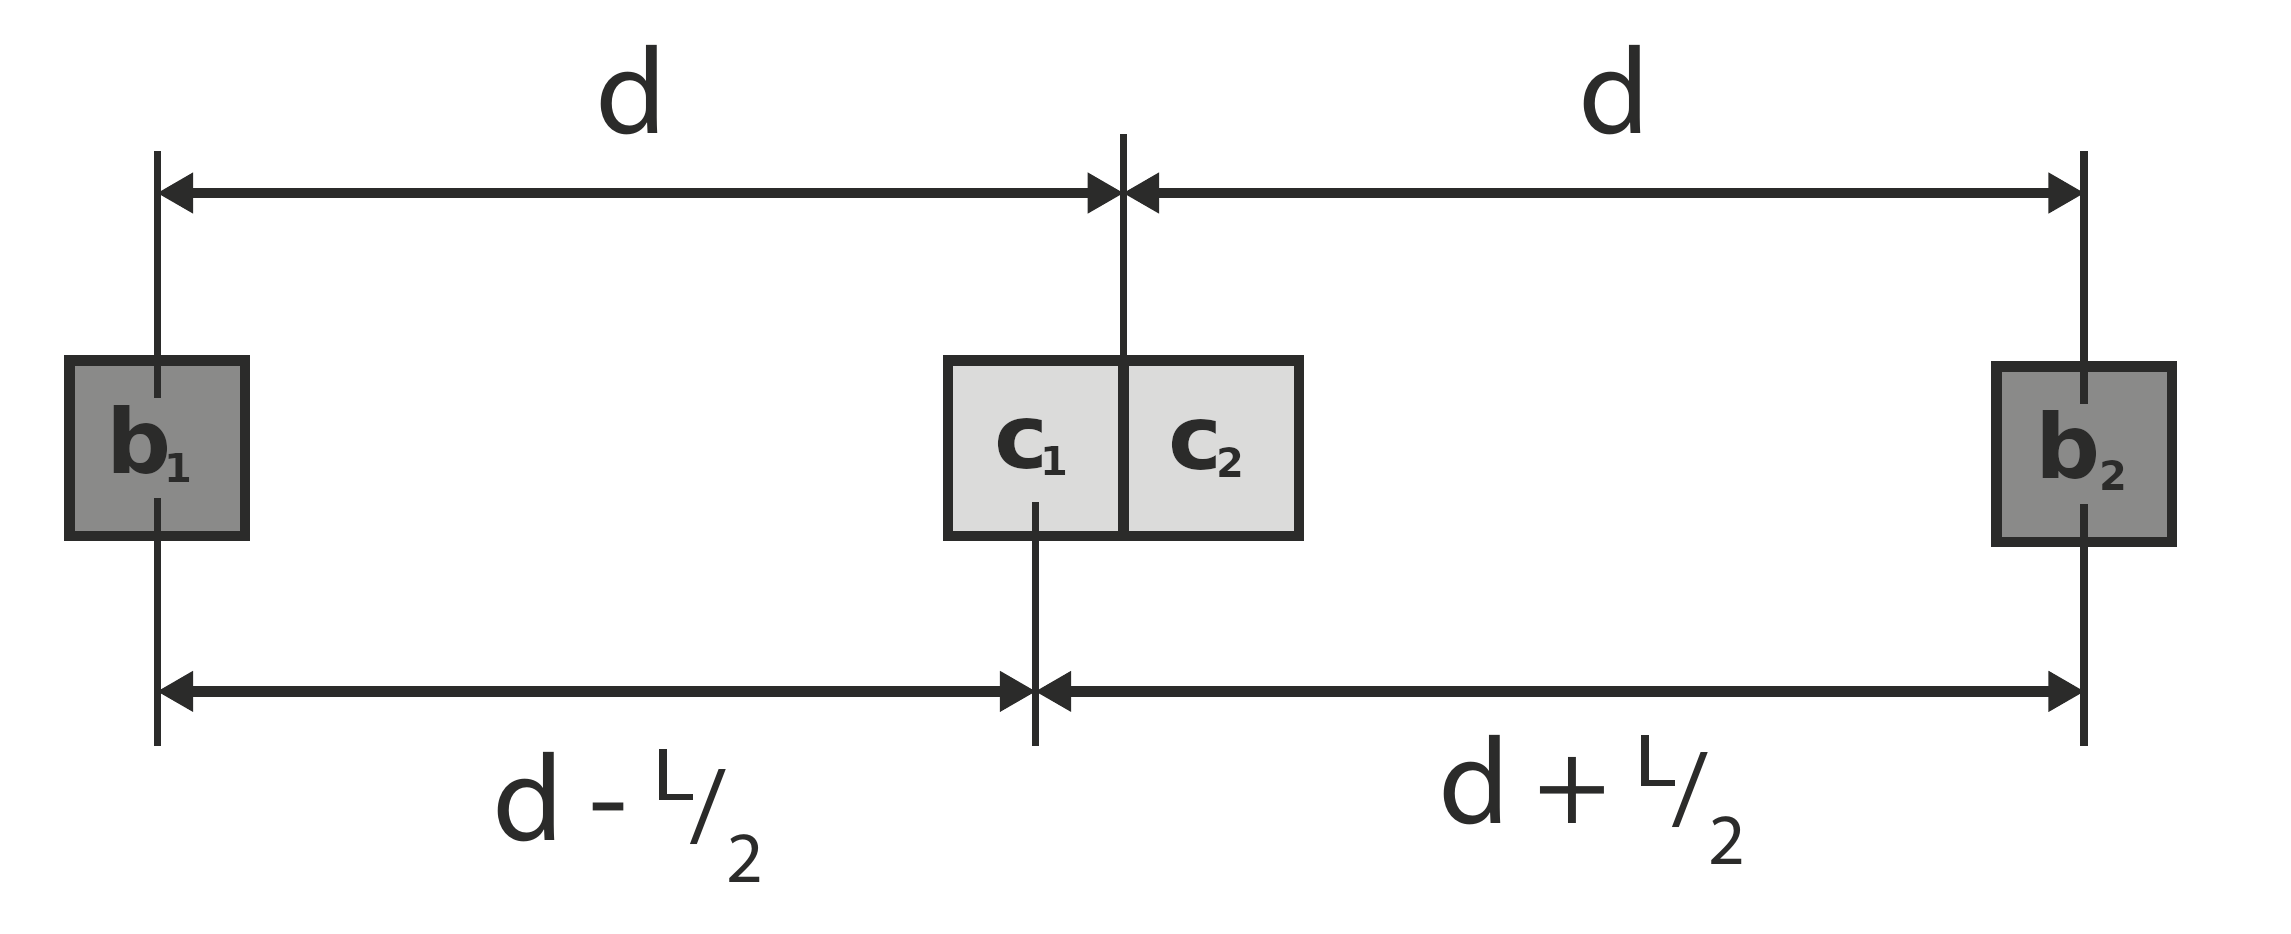
\includegraphics[clip=true, width=0.80\textwidth]{imagenes/basis/horizontalMod.png}

  \caption[Caso en el cual se requiere de una tolerancia para detectar correctmente a las celdas base.]{Caso en el cual se requiere de una tolerancia para detectar correctamente a las celdas base. Modificada de \cite{Liu2015}}\label{fig:bptol}

\end{figure}

La definición (\ref{eq:bpDisc}) se basa en el análisis realizado en
\cite{Liu2015} donde se resuelve que la la tolerancia debe ser $L$.

% Con el motivo de incluir celdas como $b_2$ que por
% causa de la discretizacion no estan a una mínima distancia $DD(c)$ de $c$ en
% $DBP_c$ . 
% Adaptar directamente la definicion de punto base en espacio continuo a celda base en el espacio discreto resulta en que solo
% las celdas que estan a una distanicia $\mli{DD}(c)$ de $c$, son las que estan a
% mínima distancia de $c$, estas serían las unicas celdas base de $c$ si se adaptara de
% forma directa la definicion de punto base en espacio continuo. Sin embargo al adaptar
% de forma directa la definicion existen casos donde los resultados difieren de
% los que se obtienen en el espacio continuo. 
% Un ejemplo es caso que se presenta en la figura \ref{fig:bptol} donde se tiene
% una seccion horizontal de un corredor. En el espacio continuo esto genera la
% pertenecia de los puntos del centro del corredor al GVD, donde cada punto $p$
% que pertenece al GVD tiene dos puntos base, uno a cada lado del corredor a
% distancia $d$ de $p$. El problema ocurre cuando la discretizacion de dicho
% corredor resulta en un número par de celdas libres entre cada celda ocupada
% correspondiente a una pared del corredor, en este caso se tendran dos celdas
% $c_1$ y $c_2$ en el centro del corredor, $c_1$ tiene una celda $b_1 \in CGen$ a
% mínima distancia $d_c(b_1) = DD(c) = d-\frac{L}{2}$, mientras que la celda $b_2
% \in CGen$ está en el otro lado del corrdor a distancia $d_c(b_2) =
% d+\frac{L}{2}$, según lo que ocurre en el espacio continuo esta
% deberia ser tambien una celda base aunque no este a mínima distancia de $c$. La
% tolerancia introducida en la definicion presentada en (\ref{eq:bpDisc}) asegura
% la pertenencia de $b_2$ a $CGen$, recordadndo que $b_2\in CGen$ entoces según
% dicha definicion se tiene que:


 % Debido a la discretizacion  no lleva a buenos resultados ya que la defincion de
% celda base agrega una tolerancia que permite una correcta generacion del GVD
% discretizado, esta tol

% a celda base sería entoces la celdas pertenecientes a un generador tal que su distancia
% , y dado que $minD$ de
% dichas deldas más cercanas a $c$, tambien se incluyen las celdas que estan a $minD+L$

% 1 defino minD 

% 2 expreso la def en paralabra

% 3 eq

% 4 explico la relacion con la variante continua y el porque de la toreancia (dibujito de liu ming)

% (notar que no es relevante saber a que
% generdor pertnece cada punto)
% \todo{explicar
% problemas de dicretizacion (ming-siegwart)}.

Finalmente las \emph{líneas críticas discretizadas} se definen como las líneas
discretizadas \cite{foleyphillips} definidas entre los centros de las celdas
críticas y los centros de cada una de sus celdas base. El conjunto de todas las
celdas pertenecientes a alguna línea crítica discretizada se conoce como
$\mli{LCrD}$.

Una vez determinadas las celdas críticas y las líneas críticas discretizadas es
posible obtener la segmentación del entorno. Esto se hace aplicando un
algoritmo de descomposición en componentes conexas (sección
\ref{subsec:CompComp}) donde cada componente conexa resultante es un segmento, y
el conjunto que se descompone es el que está compuesto
por las celdas libres de $\mli{CG}$ que no son celdas críticas ni forman parte
de una línea crítica discretizada, es decir:
\begin{align*}
\{ c \in \mli{CG} : estado(c) = libre, c \notin \mli{CCr}, c \notin{LCrD}\}
\end{align*}

En la figura \ref{fig:ejSegGVDGrid} se muestra el proceso de segmentación
completo, desde la grilla de ocupación usada como entrada
\ref{fig:ejSegGVDGrid:GRID}, pasando por el GVD generado
\ref{fig:ejSegGVDGrid:GVD}, la detección de celdas críticas y líneas críticas discretizadas
\ref{fig:ejSegGVDGrid:CRI}, y terminando con la segmentación del entorno
\ref{fig:ejSegGVDGrid:SEG}.

\begin{figure}[H]
  \centerfloat

  \subfloat[Grilla de ocupacion]{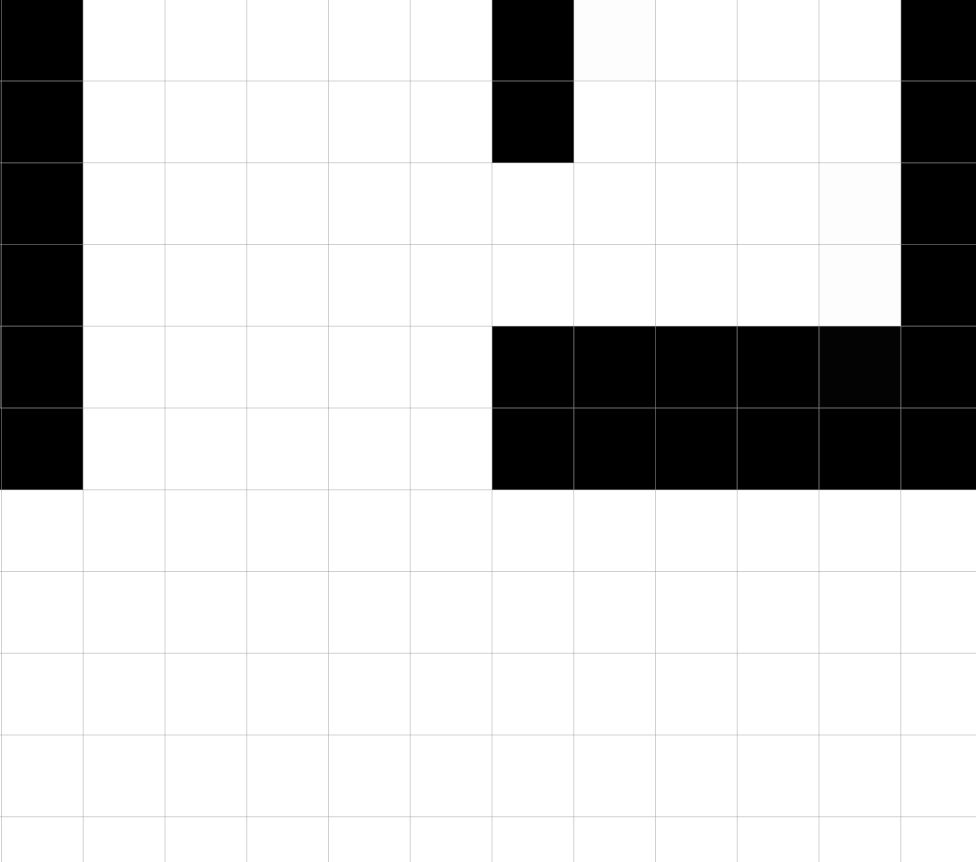
\includegraphics[clip=true,
  width=0.40\textwidth]{imagenes/GVDDisc/a.png}\label{fig:ejSegGVDGrid:GRID}}
  \qquad
  \subfloat[GVD]{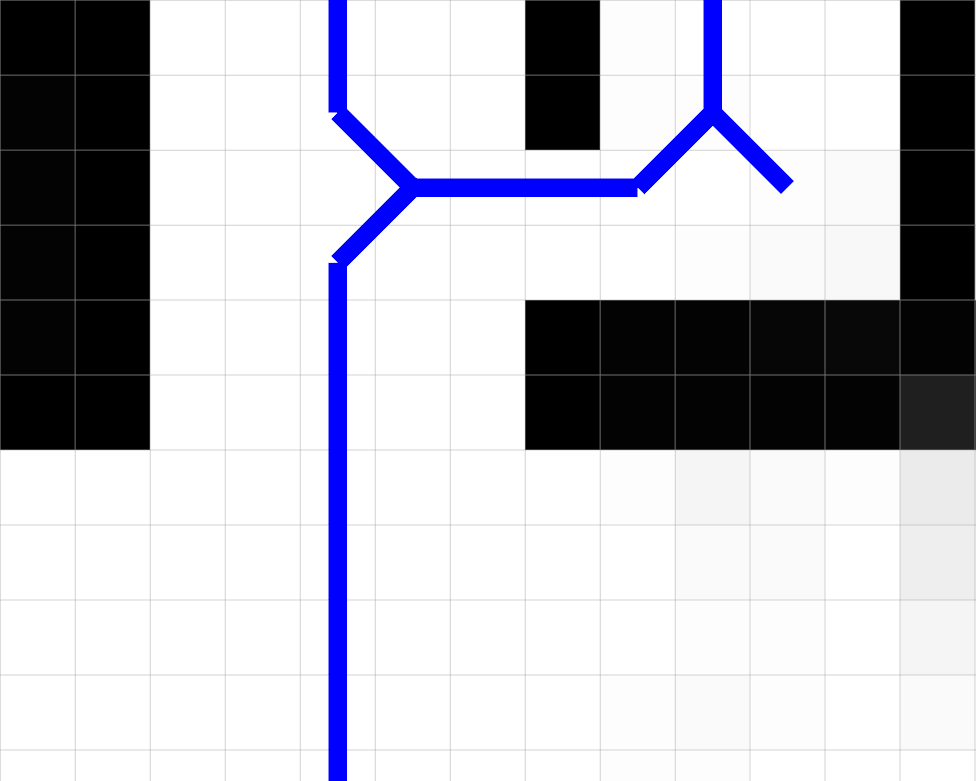
\includegraphics[clip=true,
  width=0.40\textwidth]{imagenes/GVDDisc/b.png}\label{fig:ejSegGVDGrid:GVD}}

  \subfloat[Celdas críticas, contienen cuadrados amarillos. Y celdas pertenecientes a líneas críticas discretizadas, contienen cuadrados grises]{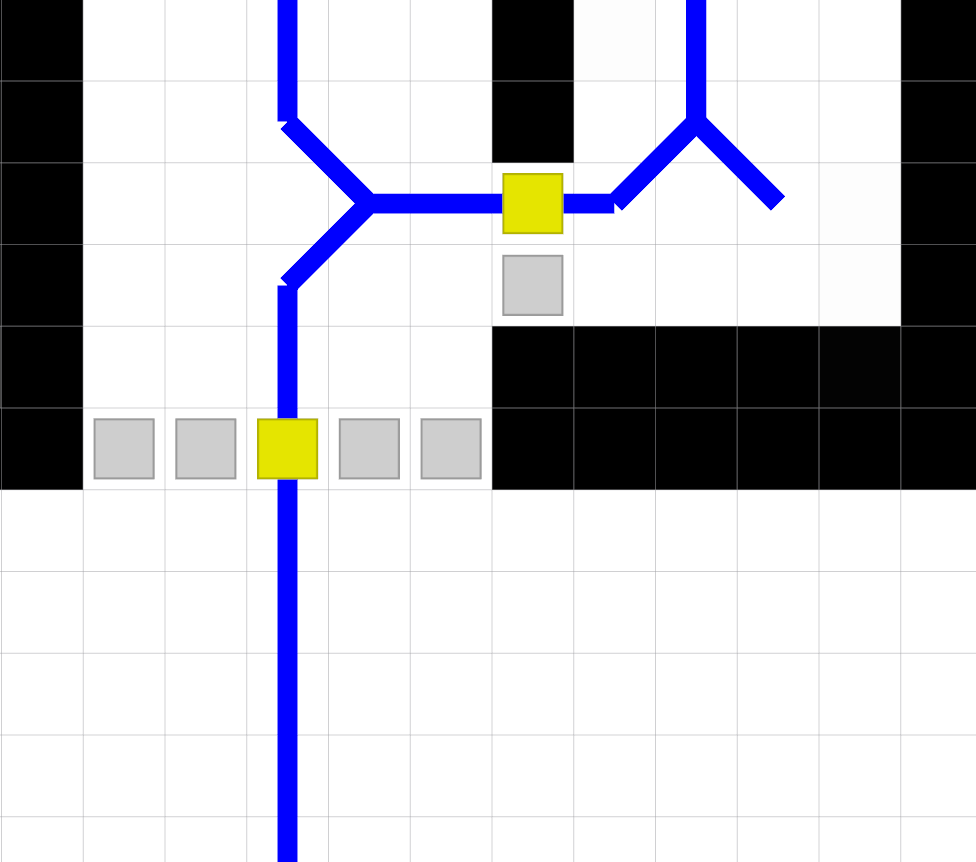
\includegraphics[clip=true, width=0.40\textwidth]{imagenes/GVDDisc/c.png}\label{fig:ejSegGVDGrid:CRI}}
  \qquad
  \subfloat[Segmentación del entorno, cada segmento se indica con un
  color distinto]{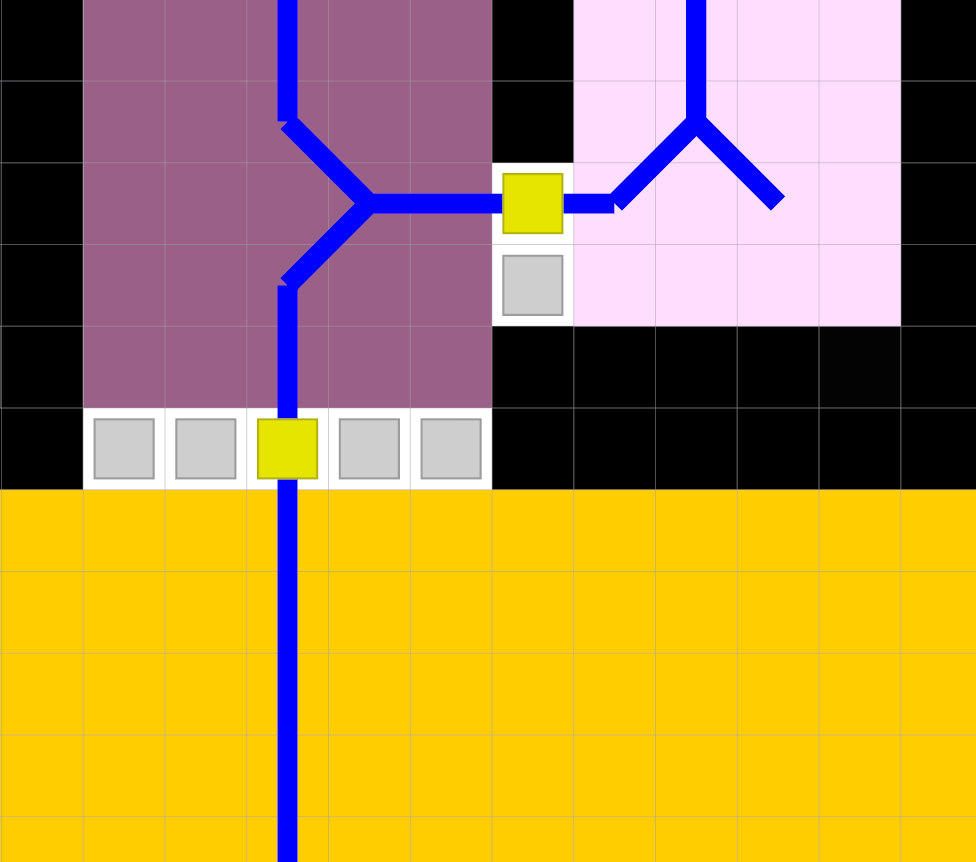
\includegraphics[clip=true,
  width=0.40\textwidth]{imagenes/GVDDisc/d.png}\label{fig:ejSegGVDGrid:SEG}}

  \caption{Proceso de segmentación de un entorno representado con una grilla.}\label{fig:ejSegGVDGrid}

\end{figure}


Una consideración a tener en cuenta es que para obtener una segmentación
correcta el algoritmo \ref{alg:compcon} debe ejecutarse con $ady_4$ como
función de adyacencia (sección \ref{subsec:Grilla}), ya que si se usa $ady_8$
las líneas críticas discretizadas diagonales no separan segmentos. Esto se debe
a que siempre existen celdas a ambos lados de una línea discretizada diagonal que son
adyacentes diagonalmente como se muestra en la figura \ref{fig:probDiagSeg}. De
usarse $ady_4$ las líneas críticas diagonales sí separan segmentos al no estarse
permitiendo la adyacencia diagonal.

\begin{figure}[H]
  \centerfloat

% , c es adyacente a n3, lo que causa un único segmento.

  \subfloat[Usando $ady_8$]{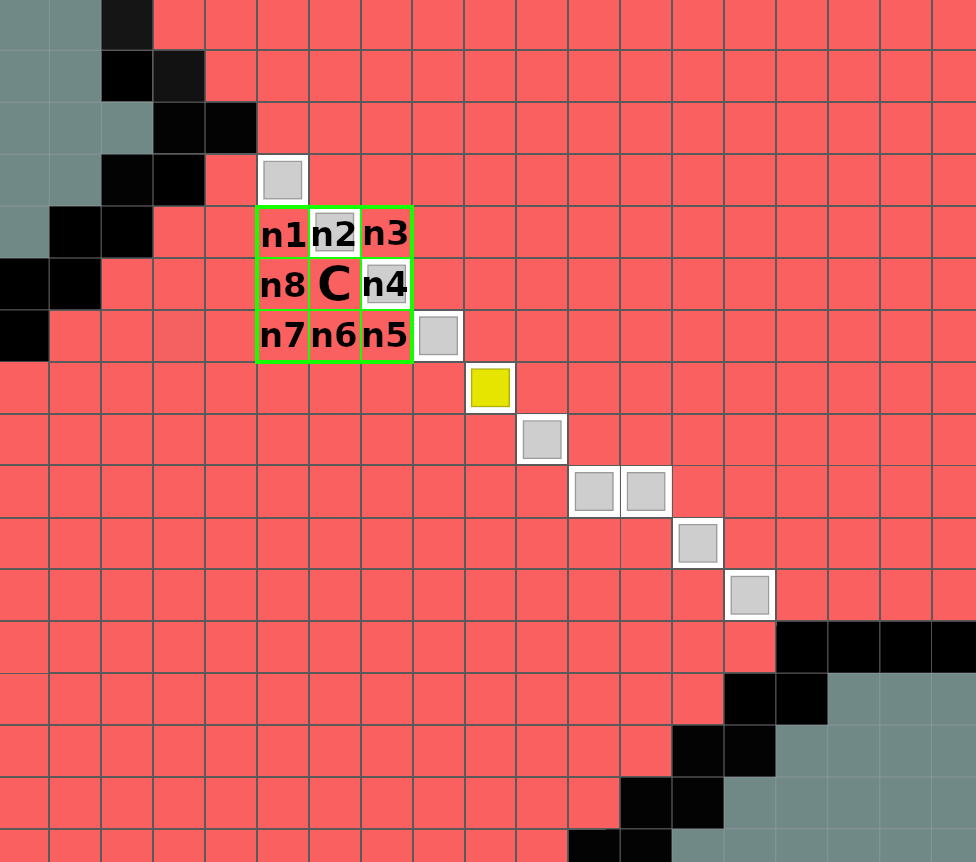
\includegraphics[clip=true, width=0.40\textwidth]{imagenes/probDiagSeg/0_33_8conRojov3.png}}
  \qquad
  \subfloat[Usando $ady_4$]{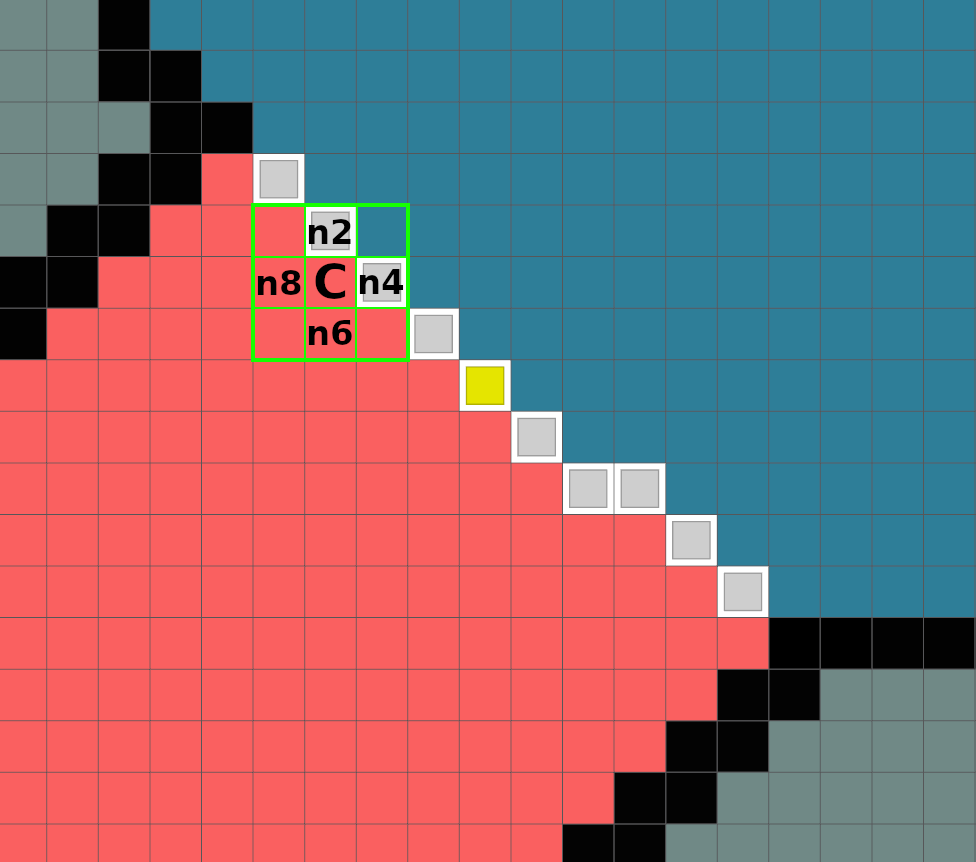
\includegraphics[clip=true, width=0.40\textwidth]{imagenes/probDiagSeg/0_33_4con.png}}

  \caption[Línea crítica discretizada diagonal, y sus efectos en la
  segmentacion al usar $ady_4$ o $ady_8$.]{Línea crítica discretizada diagonal, y sus efectos en la
  segmentación al usar $ady_4$ o $ady_8$. La celda $c$ es un ejemplo de
una celda a un lado de la línea que es adyacente según $ady_8$ a la celda $n3$ al 
otro lado de la línea, cosa que no sucede con $ady_4$.}\label{fig:probDiagSeg}

\end{figure}

% Antes de terminar esta sección una aclaración que es pertinente es que en este
% capítulo el termino GVD refiere a GVDD. 

% Tambien se filtran las líneas críticas, como las ideas es que estas se ubiquen en umbrales 

% Desribir problemas de desconexion presentados en las diversas implementaciones? 
% \begin{itemize}
%   \item mencionar los de kalra?
%   \item los generados por considerar dist 1 en lau?
%   \item y mostrar que liu ming aunque no explique que hace bien tambien los tiene?
% \end{itemize}

% Aunque existe una etapa de erosion posterior como en Lau para asegurar la
% sparceness. Comentar que se basa en el A de zhang, que en principio es más
% eficiente que chequear patrones

% Se mantienen todos los obts a mínima distancia, y los que \say{casi} estan a
% mínima distancia, siendo estos los puntos bases (puntos más cercanos a
% generadosres base) tomados en cuenta, según estos se define si un punto pertenece o no al GVD.



\section{Grafo generalizado de Voronoi}\label{sec:MiConstGVD}

Considerando los problemas de eficiencia del algoritmo no incremental de
construcción del GVD llamado \emph{brushfire} (sección \ref{subsec:constGVD}), y los
problemas de su variante incremental denominada \emph{brushfire dinámico} (sección
\ref{subsec:constGVDInc}) como se propone originalmente en
\cite{kalra2009incremental}. Se decidió basar la construcción del GVD en la
versión de \emph{brushfire dinámico} propuesta en \cite{Lau2013}, a la que se
estará haciendo referencia cuando se mencione \say{\emph{brushfire dinámico}
original} desde este punto.

% (que se
% corresponde con la función de despeje discretizado $\mli{DD} : \mli{CG}
% \rightarrow \mathds{R}$)

La implementación realizada en este proyecto mantiene el concepto de ondas
consistentes e inconsistentes del \emph{brushfire dinámico} original para el
calculo incremental de un mapa de distancia. Adicionalmente mantiene que dichas
ondas consistentes e inconsistentes remueven del GVD a las celdas que
atraviesan, y que las celdas candidatas a pertenecer al GVD son las celdas en
las que ocurren choques de ondas consistentes.

Los cambios principales respecto al \emph{brushfire dinámico} original se dan
en el criterio con el cual se determina la pertenencia de las celdas candidatas
al GVD y en como se considera el espacio desconocido al construir el GVD
durante la exploración. Estos se tratan en las siguientes secciones.

\subsection{Criterio de pertenecía}\label{subsec:critPer}

En el \emph{brushfire dinámico} original la pertenecía de las celdas al GVD se
determina en los choques de ondas consistentes. Dada la función $\mli{gen} :
\mli{CG} \rightarrow \mli{CGen}$ que para cada celda $c$ de la grilla devuelve
una de las celdas que pertenecen a un generador que están a mínima distancia de $c$, el
criterio de pertenecía original esencialmente consiste en que, sean $c_1$ y $c_2$ las celdas
involucradas en un choque de ondas consistentes, estas pertenecen al GVD si
$\mli{gen}(c_1) \neq \mli{gen}(c_2)$ y $\mli{gen}(c_1) \notin
ady(\mli{gen}(c_2))$, es decir si $\mli{gen}(c_1)$ y $\mli{gen}(c_2)$ no son
iguales ni adyacentes entre sí. 

% Recordando que los  
% puntos base son los puntos pertenencientes parte de los puntos base de $p$ (sección
% \ref{subsec:mapaTopGVDGrid}).

% La definición de GVD para el espacio continuo establece que un punto $p$
% pertenece al GVD si tiene al menos dos generadores distintos a mínima
% distancia, lo cual sucede si y solo si $p$ tiene al menos dos puntos a mínima distancia
% pertenecientes a generadores distintos. Dado esto se puede decir
% que un punto pertenece al GVD si tiene al menos dos puntos base (sección
% \ref{subsec:mapaTopGVDGrid}) que pertenecen a generadores distintos, lo cual en
% un espacio discretizado en celdas se traduce a que existan dos celdas base que
% pertenecen a generadores
% distintos.

La definición de GVD para el espacio continuo establece que un punto $p$
pertenece al GVD si tiene al menos dos generadores distintos a mínima
distancia, lo cual sucede si y solo si al menos dos de los puntos pertenecientes a
generadores, que están a mínima distancia de $p$ pertenecen a generadores
distintos. Dado esto se puede decir que un punto pertenece al GVD si tiene al
menos dos puntos base (sección \ref{subsec:mapaTopGVDGrid}) que pertenecen a
generadores distintos, que en un espacio discretizado en celdas se traduce
a que una celda tenga dos celdas base que pertenecen a generadores distintos.

 % del \emph{brushfire dinámico} original
Dado este análisis y la necesidad de determinar las celdas base que fue
planteada en la sección \ref{subsec:mapaTopGVDGrid}, se decidió cambiar el
criterio de pertenencia al GVD, siendo el nuevo criterio de pertenencia de una
celda al GVD que al menos dos de sus celdas base pertenezcan a generadores
distintos.

% choque de ondas, de forma similar al criterio de pertenencia de celdas al GVD en
% el \emph{brushfire dinámico} original.
Las celdas base se obtienen en los choques de ondas consistentes. En cada
actualización del mapa de distancia correspondiente a un incremento, se
registran todas las celdas involucradas en choques de ondas consistentes.
Luego de finalizar la actualización del mapa de distancia, con el algoritmo
\ref{alg:celdasBase} se obtienen las celdas base $\mli{CB}_c$ de cada celda $c$
registrada previamente. Notar que la función de despeje discretizada $\mli{DD}
: \mli{CG} \rightarrow \mathds{R}$ se corresponde los valores del mapa de
distancia calculado.

\begin{algorithm}[H]
\SetAlgoLined
  \SetKwInOut{Input}{Entrada}
  \Input{$c$}

% En updateBase c es pN y cA es p
% En setPseudoSourcesFromWave c es p y cA es waveP

  $\mli{minD} := \infty$

  % \tcp{DFS desde $c$ agregando las celdas visitadas a la componente conexa $C_i$}
  \ForEach{ $cA \in ady(c)$} {
    $b := \mli{gen}(cA)$\\
    $\mli{tolerado} := d_c(b) \leq \mli{DD}(c) + L$\\
    $\mli{noIgNiAdy} := b \neq gen(c) \land b \notin ady(gen(c))$\\
    $\mli{masCercano} := d_c(b) < minD$\\
    \If{$\mli{tolerado} \land \mli{noIgNiAdy} \land \mli{masCercano}$}{
      $\mli{minD}  := d_c(b)$\\
      $\mli{ultimo} := b$\\
    }
  }
  $\mli{CB}_c := \{\mli{gen}(c)\}$\\
  \If{$\mli{minD} < \infty$}{
    $\mli{CB}_c := \mli{CB}_c \cup \{\mli{ultimo}\}$\\
  }
  \Return $\mli{CB}_c$ 

  \caption{Obtención de las celdas base $\mli{CB}_c$ de una celda $c$ (simplificada)}
  \label{alg:celdasBase}
\end{algorithm}

El algoritmo para cada celda $cA$ adyacente a $c$ (línea 2) obtiene un
candidato a ser una celda base de $c$ (línea 3) y comprueba una serie de
condiciones utilizadas para determinar las celdas base de $c$ (líneas 4-6). La
condición que se comprueba en la línea 4 es que la celda base candidata esté
dentro del intervalo definido por la tolerancia (sección
\ref{subsec:mapaTopGVDGrid}). La condición que se verifica en la línea 5 es que
el candidato no sea $gen(c)$ ni adyacente a él. Finalmente la condición
presente en la línea 6 establece que el candidato actual debe tener una
distancia a $c$ menor a la de los candidatos procesados anteriormente que
cumplieron con todas las condiciones. Al finalizar la ejecución se devuelve como
celdas bases a $gen(c)$ y en el caso de que exista al último candidato en
cumplir todas las condiciones (líneas 12-16).

%(sacr de la implementacion) (notar que gens a igual distancia tambien se encuentran, igual no comentar por las dudas)

% Notar el uso de la tolerancia de un largo de celda determinada en \cite{Liu2015}

Una vez obtenidas las celdas base de un celda $c$, para determinar la
pertenencia de $c$ al GVD resta verificar si existen dos celdas base de $c$ que
pertenecen a generadores distintos. Para esto se aplica una técnica derivada del
criterio de pertenencia de celdas al GVD presente en el \emph{brushfire
dinámico} original, que consiste en que dos celdas pertenecen a distintos
generadores si son distintas y no adyacentes entre sí, y de lo contrario
pertenecen al mismo generador. 
De esta forma se logra obtener incrementalmente tanto el GVD, como las celdas
base necesarias para segmentar.
% De esta forma se logra aproximar el GVD resultante de considerar generadores
% conexos y convexos (sección \ref{subsec:GVD}) sin definir explícitamente los
% generadores, y adicionalmente se obtienen las celdas base que son necesarias
% para segmentar.

% , de forma similar al criterio de pertenecía del \emph{brushfire dinámico} original
% para obtener las celdas base
Es pertinente aclarar que el algoritmo \ref{alg:celdasBase} es una versión
simplificada del que está presente en la implementación del proyecto. Las
simplificaciones son dos, la primera es que para cada celda $cA$ adyacente a
$c$ solo se considera como candidata a una de las celdas pertenecientes a un
generador que están a mínima distancia de $cA$ (la resultante de $gen(cA)$). Y
la segunda es que solo se permiten hasta dos celdas base. En la sección
\ref{algComp:celdasbase} se presenta el algoritmo completo sin las
simplificaciones mencionadas, es decir que considera como candidatas a todas
las celdas que pertenecen a un generador que están a mínima distancia,
y permite más de dos celdas base.

\subsection{Consideraciones sobre el espacio desconocido}\label{subsec:espDesc}
% , dichas celdas representan la existencia de porciones del mapa cuyo
% contenido se desconoce.

Mientras la exploración está en curso existe espacio desconocido del entorno
que puede ser explorado, este se representa con celdas de estado desconocido en
la grilla de ocupación (sección \ref{subsec:Grilla}) usada como mapa del
entorno. Dado que la definición del GVD (sección \ref{subsec:GVD}) no contempla
el espacio desconocido, para poder construir un GVD sobre una grilla de
ocupación durante la exploración, es necesario decidir como considerar las
celdas de estado desconocido.
Sin embargo, este no es un tema que se trate de forma explicita en los trabajos
estudiados sobre la construcción incremental del GVD (sección \ref{subsec:constGVDInc}). 

A partir de código e imágenes disponibles es posible deducir que en
\cite{kalra2009incremental} y \cite{Lau2013} al construir el GVD las celdas de
estado desconocido se consideran iguales a las de estado libre. De esta
forma se obtienen resultados similares al que se presenta en la figura
\ref{fig:kalraOG}. Notar que otra característica particular presente en estas
implementaciones es que las celdas ubicadas en los bordes del entorno se
consideran como pertenecientes a generadores.

\begin{figure}[H]
  \centerfloat

  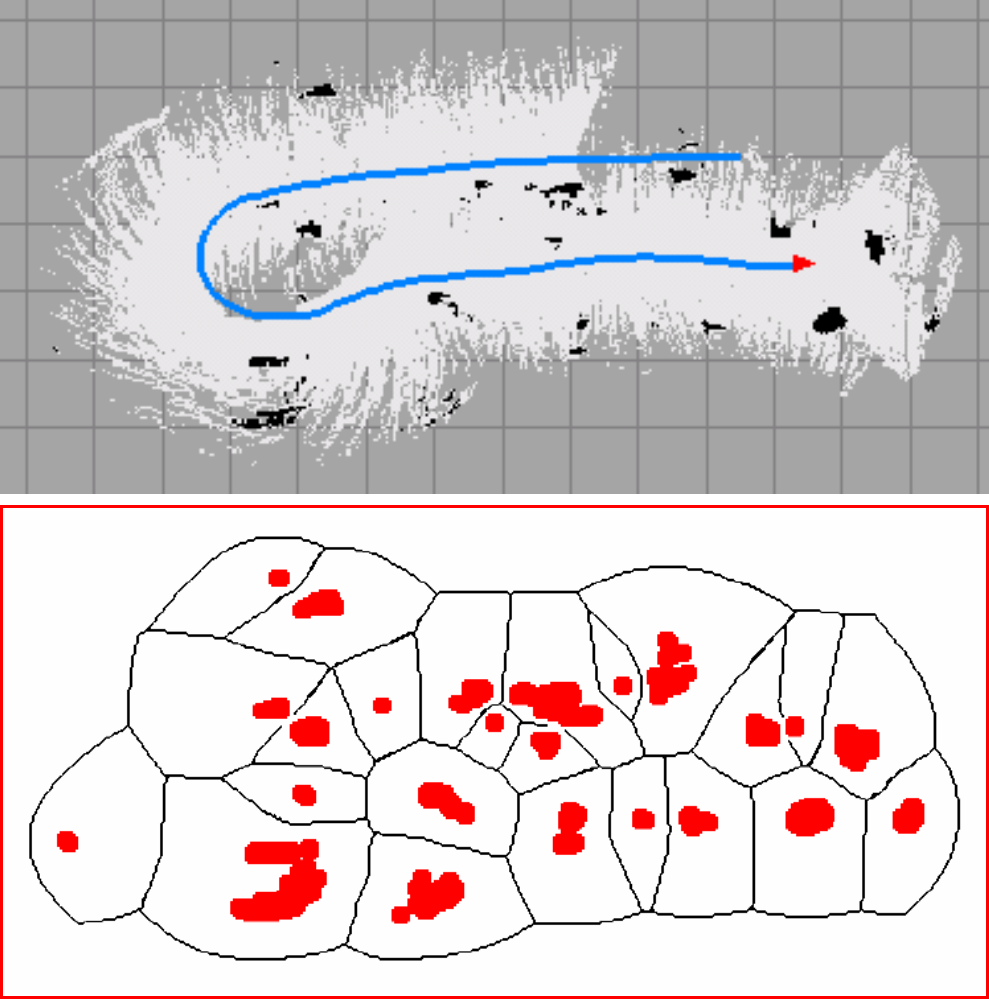
\includegraphics[clip=true, width=0.75\textwidth]{imagenes/desconocidoCons/kalraOG.png}

  \caption[Resultado de considerar las celdas de estado desconocido iguales a las de estado libre.]{Resultado de considerar las celdas de estado desconocido iguales a las de estado libre. En la parte superior se muestra la grilla de ocupación actual. En la inferior su GVD correspondiente, indicándose con rojo los obstáculos. Extraída de \cite{kalra2009incremental}.}\label{fig:kalraOG}

  % \caption[Consideración del espacio desconocido presente en \cite{kalra2009incremental} y \cite{Lau2013}.]{Consideración del espacio desconocido presente en \cite{kalra2009incremental} y \cite{Lau2013}. En la parte superior se muestra la grilla de ocupación actual. En la inferior su GVD correspondiente, indicándose con rojo los obstáculos. Extraída de \cite{kalra2009incremental}.}\label{fig:kalraOG}
\end{figure}

Que las celdas desconocidas se consideren iguales a las celdas libres
implica que las ondas utilizadas para construir el GVD pueden propagarse por el
espacio desconocido y generar la pertenecía de celdas desconocidas al GVD.
% ambas cosas tienen asociado un costo computacional.
En la figura \ref{fig:desconocidoKalra} se puede observar que considerar las
celdas desconocidas como celdas libres lleva a un GVD que abarca
todo el entorno sin importar que solo una pequeña porción de este sea
conocida. 

%mantener un GVD conexo,
% (por motivos que se seran comentados a continuacion)

Dado que en el contexto del proyecto no es necesario construir el GVD fuera del
área conocida, se desarrollo un método que solo construye el GVD en las celdas
libres, evitando el costo computacional de construir el GVD en el espacio
desconocido. Sea $\mli{UF}$ el conjunto de celdas desconocidas que tienen al menos una
celda adyacente de estado libre, el método consiste en considerar que las
celdas desconocidas no propagan ondas, y que las celdas de $\mli{UF}$
pertenecen a generadores ($\mli{UF}\subseteq \mli{CGen}$) al igual que las
celdas ocupadas. Con este método para el caso presentado en la figura
\ref{fig:desconocidoKalra} se obtiene un GVD que se reduce al espacio conocido
como se muestra en la figura \ref{fig:desconocidoMio}.
% evitando propagar las ondas sobre el espacio desconocido, 

\begin{figure}[H]
  \centerfloat

  \subfloat[Celdas desconocidas se consideran como libres.]{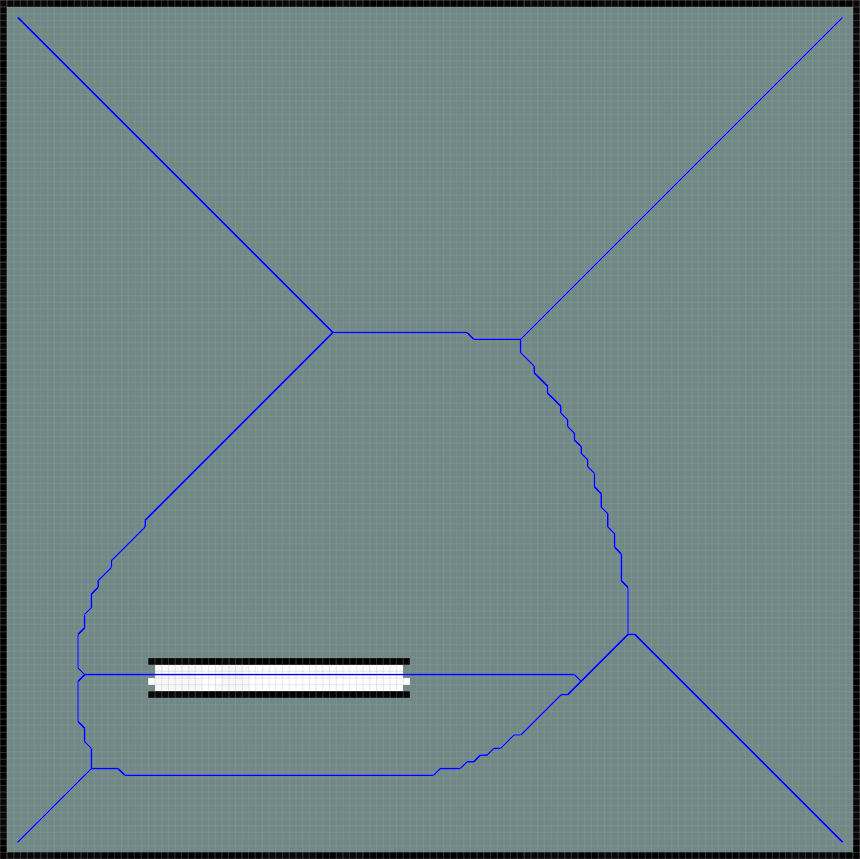
\includegraphics[clip=true, width=0.45\textwidth]{imagenes/conectividad/kalra.png}\label{fig:desconocidoKalra}}
  \quad
  \subfloat[Celdas desconocidas no propagan ondas y $\mli{UF}\subseteq \mli{CGen}$.]{
\includegraphics[clip=true, width=0.45\textwidth]{imagenes/conectividad/mio.png}\label{fig:desconocidoMio}}

  \caption[Formas de considerar el espacio desconocido.]{Formas de considerar el espacio desconocido. El GVD generado se indica en azul.}\label{fig:desconocidoEj1}
\end{figure}

% , en una misma
% grilla de ocupación

Considerar únicamente que las celdas desconocidas no propagan ondas también
restringe la construcción del GVD al espacio conocido, aunque esto puede ser
más simple e intuitivo tiene el problema de generar GVD disconexos en casos
donde esto se puede evitar. El problema con los GVD disconexos es que estos no
cumplen con la propiedad de \emph{conectividad} necesaria para ser un
\emph{roadmap} (sección \ref{subsec:mapacarr}), lo que genera errores al
utilizar el GVD como \emph{roadmap} para la planificación. En la figura
\ref{fig:desconocidoEj2} se muestra el GVD generado con cada una de las tres
formas de considerar el espacio desconocido mencionadas hasta el momento. Es
posible observar que el GVD resultante de solo considerar que las celdas
desconocidas no propagan ondas es disconexo, mientras que el GVD generado por
otros dos métodos es conexo.

% El problema presentado por esta forma de considerar el espacio desconocido es
% que las ondas se propagan por el espacio desconocido, generado GVD fuera del

% al explorar donde en un mapa no solo hay obtaculos y celdas libres si no que tambien hay celdas desconocidas,
% Llamado de atencion al problema de conectividad de un GVD al explorar donde en un mapa no solo hay obtaculos y celdas libres si no que tambien hay celdas desconocidas, las cuales no se consideran en los articulos del estado del arte. Estos se asume (no se explicita pero en Kalra se ve que el mapa para entorno abierto es consistente con esta tecnica, en el codigo de lau tambien) que implementan la tecnica de "los limites de mi mapa son obstaculos" y lo desconocido es libre. En este trabajo se propone una tecnica novedosa que soluciona este problema de forma más eficiente evitando procesar todo el espacio desconocido mientras se va explorando.

\begin{figure}[H]
  \centerfloat

  \subfloat[Celdas desconocidas se consideran como libres.]{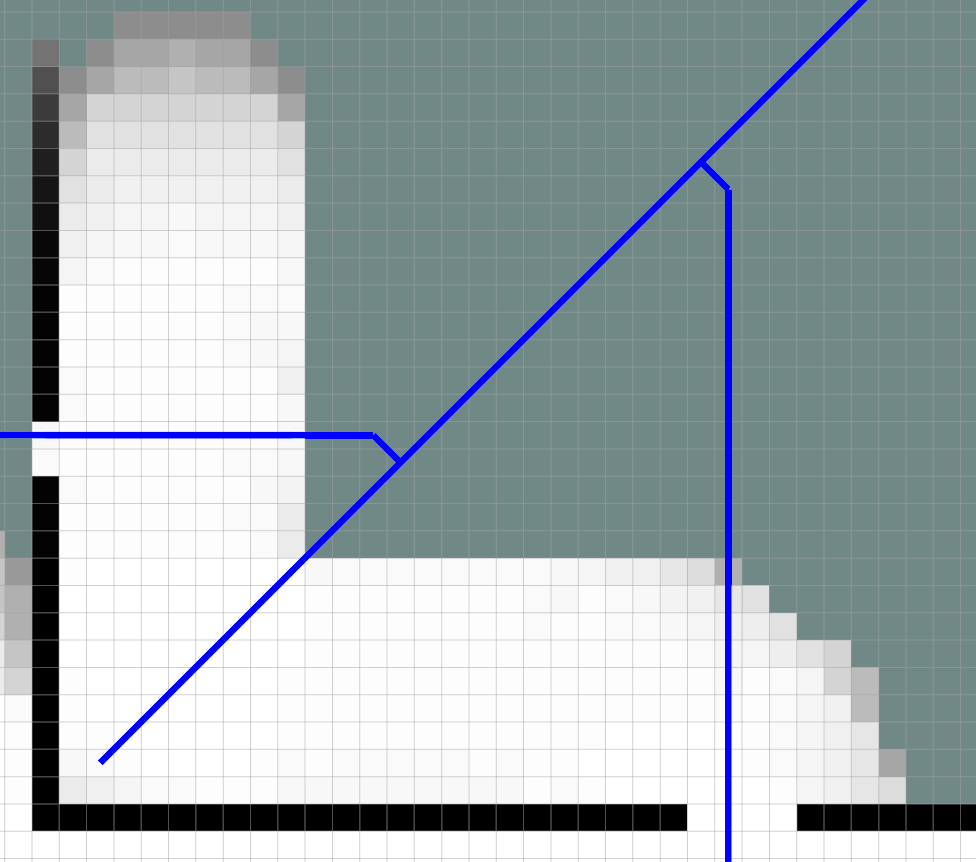
\includegraphics[clip=true, width=0.32\textwidth]{imagenes/desconocidoCons/kalra.png}}
  \quad
  \subfloat[Celdas desconocidas no propagan ondas y $\mli{UF}\subseteq \mli{CGen}$.]{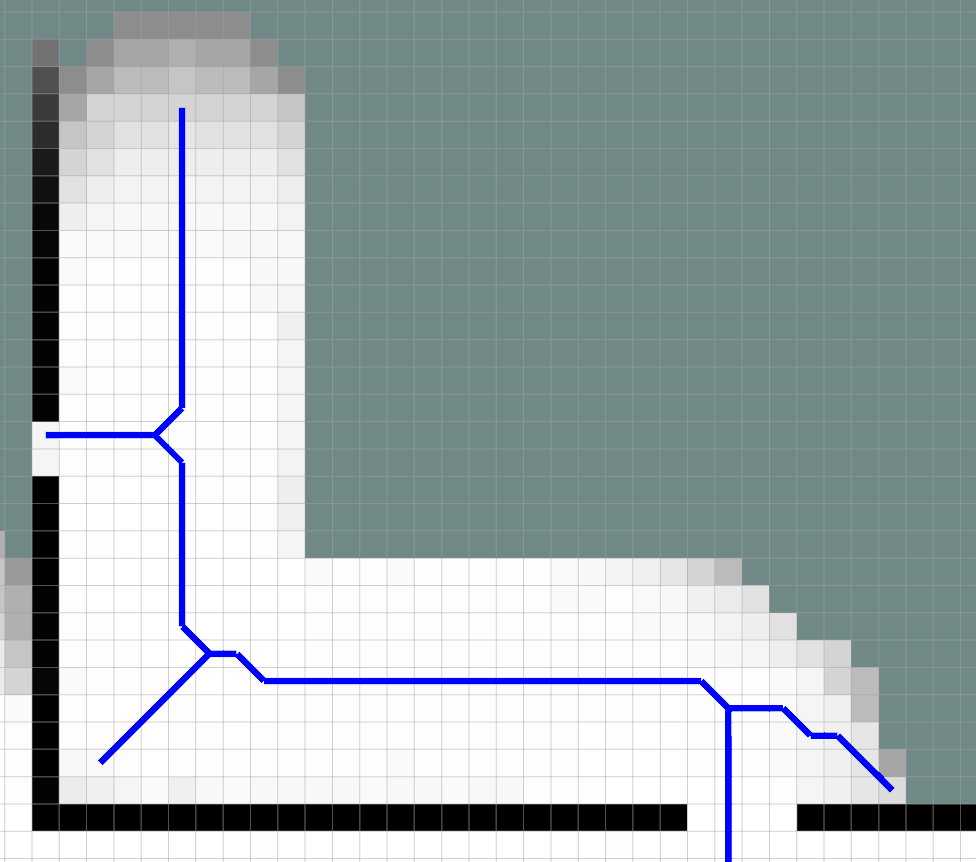
\includegraphics[clip=true, width=0.32\textwidth]{imagenes/desconocidoCons/mio.png}}
  \quad
  \subfloat[Celdas desconocidas no propagan ondas.]{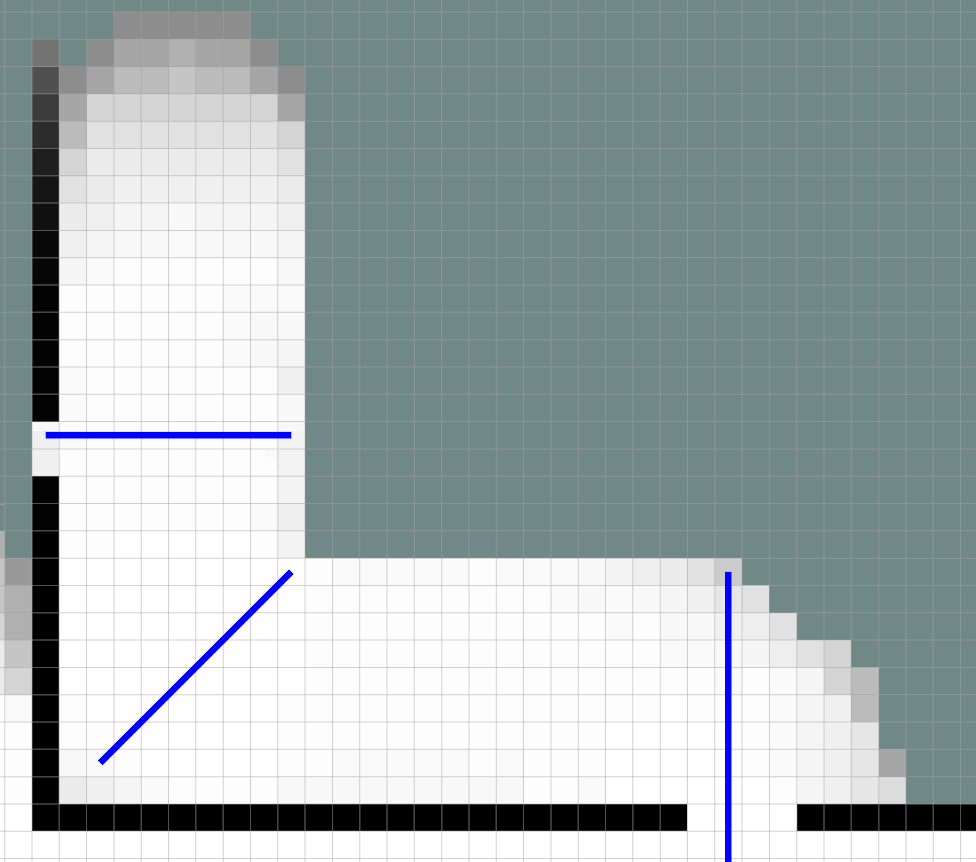
\includegraphics[clip=true, width=0.32\textwidth]{imagenes/desconocidoCons/noHacerNada.png} \label{fig:desconocidoEj2_naive}}

  \caption[Conectividad del GVD en diferentes formas de considerar el espacio desconocido.]{Conectividad del GVD en diferentes formas de considerar el espacio desconocido. El GVD generado se indica en azul.}\label{fig:desconocidoEj2}
\end{figure}

% 1. desconexiones
% 2. incrementalmente si se agregan celdas libres que no son obstaulos entonces igual es necesario actualizar el GVD

% , la alternativa de que los bordes no sean
% Obstaculos (como esta no aplica a entornos abiertos y genera más costos) y


% Explicar el problema de considerar lo desconocido, como no hacerlo lleva a GVD
% disconexos, explicar lo que se encuentra en el estado del arte (explicar como
% esta aplica para entornos abiertos) y la alternativa de que las fronteras
% (invertidas) sean emisoras de ondas consistentes e inconsistentes y lo
% desconocido no sea atravezable por las ondas y porque esto implica mucho menos
% costos para mapas cuando estos se comienzan a explorar y se componen de muchas
% celdas desconocidas.

% Comentar que las celdas con lo desconocido como punto base no genera líneas ni
% puntos críticos.

% \todo{FEDE: Kalra se ve que el mapa para entorno abierto es consistente con esta tecnica, en el codigo de lau tambien. Pero no se hace referancia a esto}

% Mostrar gvd resultantes de mapas parcialemnte explorados (muy poco explorados) y comentar como toda el área desconocida debe ser procesado por el original mientras que el mio se reduce al área exploradoa, sientod la parte importante (la del área explorada) casi igual que la otra.

\section{Planificación}\label{sec:miNav}
\todohint{Quedo bien la sección? Lo que cambie es fue dejar de hablar de puntos y pasar a hablar de subobjetivos por el tema que quedaba raro hablar de completar puntos. En la parte de jerárquica uso un poco el termino puntos pero cuidando no hablar de completarlos}

% Recordando que el camino consiste en una secuencia puntos en el espacio, en el
% contexto de la planificación estos se denominan como subobjetivos con exepcion
% del último punto llamado como objetivo.

% En el contexto de la planificación los puntos que componen el
% camino se denominan subobjetivos con exepcion del último punto que se denomina
% como objetivo.

Una vez que un robot recibe un objetivo de exploración desde la central
(sección \ref{sec:asigTar}), este debe moverse físicamente hasta el lugar
indicado para completar dicho objetivo y progresar en la exploración del entorno.

% de la memoria del robot
El módulo que se encarga de recibir objetivos de exploración es el
\emph{controlador del robot}. Al recibir un objetivo de exploración este módulo
recupera el camino que fue determinado durante la valuación de dicho objetivo
(sección \ref{subsec:MiValSub}) y lo envía al módulo \emph{controlador de
movimiento}. 

% Una que el caminno llega al módulo \emph{controlador de movimiento}
% trabaja
% junto al módulo \emph{Move Base} para lograr su comentido.

 % puntos
% del camino, son relevantes para poder llegar al objetivo.

% que se
% considera no completado al módulo \emph{Move Base} el cual se encarga de
% generar las directivas a los motores del robot para que pueda llegar de forma
% segura a dicho objetivo/subobjetivo.

% Para determinar que punto debe ser enviado a
% \emph{Move Base} el \emph{controlador de moviemiento} 

% Adicionalmente tiene la tarea de determinar cuando un punto
% se considera completado

% Especificamente el \emph{controlador de
% moviemiento} comienza enviando el primer punto del camino  En algun punto de la trayectoria hacia el
% objetivo/subobjetivo que lleva a cabo \emph{Move Base} este se considera
% completado, dado esto el siguiente objetivo/subobjetivo sin completar se envia
% a \emph{Move Base}. El proceso se repite hasta completar el objetivo,
% completando asi el camnino completo.

El módulo \emph{controlador de movimiento} interpreta cada punto que compone
al camino recibido como un subobjetivo y se encarga de decidir que subobjetivos
enviar al módulo \emph{Move Base} que es el responsable de generar las
directivas necesarias para que el robot avance hacia dichos subobjetivos. Estos
subobjetivos deben enviarse en una secuencia que permita que el robot pueda seguir el
camino hasta el objetivo de exploración. Para lograr esto, asumiendo que se tiene un criterio
que permite determinar cuando un subobjetivo se considera completado, el
funcionamiento del \emph{controlador de movimiento} consiste en determinar el
primer subobjetivo no completado del camino, enviar dicho subobjetivo a \emph{Move Base} y
esperar a que el robot avance lo suficiente para completarlo. Una vez
completado se repite el proceso con el siguiente subobjetivo sin completar, esto
sucede hasta que se completa el último subobjetivo del camino que
es el objetivo de exploración.

% Para determinar cuando un punto del camino considera completado, estos se separan  el último punto  objetivo  subobjetivos con exepcion del último punto que se denomina
% como objetivo.

\subsection{Criterios de compleción}

El \emph{controlador de movimiento} tiene dos criterios para determinar que un
subobjetivo fue completado, el criterio de compleción normal y criterio de
compleción forzosa.
% \todoerror[inline]{con punto me refiero a tarea asociada al putno:  Dos opciones (introducir antes subobj) (mejor esta) o dejar alcanzado | Creo que es mejor el termino completado porque alcanzar me da una idea de cercanía que no es necesariamente el caso. Entiendo que quizás queda raro hablar de completar un punto del camino, pero esto se aclara a lo largo de la sección (y era el termino que se estaba manejando antes de comenzar la subsection) | alcanzado?}

La compleción forzosa ocurre cuando el robot está a una distancia menor a
$\mli{DistF}$ del subobjetivo en cuestión. Este criterio de compleción tiene como
propósito determinar cuando un robot está lo suficientemente cerca de un subobjetivo
 como para considerarlo completo, a pesar de que no se dio aún la
compleción normal. Se recomienda que el valor $\mli{DistF}$ sea similar a las
dimensiones del robot.
% \todoerror[inline]{similar a lo anterior|similar a lo anterior, aunque acá si esta lo de cercanía, me parece mejor completar para ser consistente | que se ha alcanzado el objetivo?}

Por otro lado para la compleción normal existen dos condiciones, la primera es
que la línea de ancho $\mli{An}$ que existe entre el robot y el subobjetivo,
al discretizarse en celdas no contenga ninguna celda ocupada. La segunda, en el
caso del objetivo de exploración es que la distancia entre este y
el robot sea menor a $\mli{DistNo}$, y en el caso del resto de los subobjetivos
es que la distancia hacia estos sea menor a $\mli{DistNs}$.

El valor $\mli{DistNo}$ debe cumplir con $\mli{DistF}\leq\mli{DistNo}<\mli{rango}$, siendo
$\mli{rango}$ el alcance de los sensores del robot. Esto se debe a que la idea
detrás del criterio de compleción normal aplicado al objetivo de exploración, es
considerar que este es completado cuando es seguro que fue sensado por el robot.
Esto implica que el robot está en condiciones de recopilar la nueva información
del entorno asociada al objetivo, siendo este el motivo por el cual el objetivo
fue asignado en un primer lugar.

El valor $\mli{DistNs}$ debe cumplir con $\mli{DistF}\leq\mli{DistNs}$, y
establece que tan estrictamente se sigue el camino original en espacios
despejados de obstáculos. Valores pequeños de $\mli{DistNs}$ hacen que el robot
siga el camino original de forma estricta aunque esté en espacios despejados,
ya que se fuerza que el robot se acerque a los subobjetivos para completarlos.
Al aumentar el valor de $\mli{DistNs}$ se permite mayor libertad en como seguir
el camino original cuando el espacio está despejado. Esto sucede porque en los
espacios despejados la línea de ancho $\mli{An}$ no se solapa con obstáculos y
por lo tanto todos los subobjetivos del camino que estén a una distancia menor
a $\mli{DistNs}$ se consideran completados. Completar varios subobjetivos a la
vez implica libertad de movimiento, al ser \emph{Move Base} el que se encarga
de la trayectoria hasta el primer subobjetivo no completado del camino, sin ser
necesario pasar por los subobjetivos previamente completados.

\subsection{Planificación jerárquica}
% es que los caminos originales
% calculados sobre el GVD (seccion \ref{subsec:MiValSub})
Los GVD son estructuras que se representan con un cantidad considerablemente
menor de celdas que las presentes en las grillas de ocupación sobre las cuales son
generados. A pesar de esto los GVD son \emph{roadmaps} (sección
\ref{subsec:mapacarr}) por lo que permiten planificar caminos entre cualquier
par de puntos del espacio, al igual que las grillas de ocupación. 

La diferencia de tamaños entre las estructuras implica que generar caminos
sobre el GVD es computacionalmente más eficiente que generarlos sobre la grilla
de ocupación. Pero a su vez, los caminos generados sobre el GVD se mantienen lo
más alejado posible de los obstáculos (sección \ref{subsec:GVD}), lo que lleva
a caminos que aunque son seguros, pueden resultar innecesariamente largos.

La motivación de la planificación jerárquica es aprovechar la eficiencia de
generar caminos sobre el GVD, evitando los desvíos innecesarios que estos
caminos contienen.

La planificación jerárquica está basada en un camino de alto nivel construido a
partir de información topológica del camino generado sobre el GVD.
El camino de alto nivel esta formado por la secuencia de los puntos del camino sobre
el GVD que se encuentran en las transiciones entre segmentos (habitaciones
y corredores), finalizando con el objetivo. Luego se establecen caminos de bajo
nivel entre el robot y el siguiente punto del camino de alto nivel, la idea de
estos caminos es que el robot pueda navegar libremente (sin considerar el GVD)
dentro de los segmentos, moviéndose de transición en transición. La
planificación de los caminos de bajo nivel se delega a \emph{Move Base} que
genera caminos sin desvíos innecesarios.

Es pertinente notar que en la implementación realizada \emph{Move Base} se
configuró con un \emph{global\_planner} (sección \ref{subsec:move_base}) que
calcula caminos sobre la grilla de ocupación, de igual manera utilizar la
planificación jerárquica simplifica los cálculos de los caminos sobre la grilla,
ya que hace que sean locales al segmento que se debe transitar. %(se usa $A^*$).

% (mayor a las dimensiones de los segmentos) 
Recordando que los caminos no triviales (sección \ref{subsec:MiValSub}) que llevan a un objetivo de exploración, enviados desde el
\emph{controlador del robot} al \emph{controlador de movimiento} son caminos
generados sobre el GVD. Para llevar a cabo la planificación jerárquica se
establece $\mli{DistNs}=\infty$ y $\mli{An}$ mayor al tamaño estimado de los
portales de transición entre segmentos (puertas, pasajes abiertos). De esta
forma asumiendo segmentos despejados, exceptuando al objetivo de exploración todos los subobjetivos asociados a un
segmento en el que se encuentra un robot son completados de forma normal. Por
lo tanto en caminos largos que abarcan varios segmentos, nuevamente exceptuando al objetivo de exploración, los únicos
subobjetivos enviados a \emph{Move Base} son los que se ubican en las
transiciones entre un segmento y el siguiente. Estos subobjetivos no son
completados de forma normal ya que dichas transiciones consisten en portales de
ancho menor a $\mli{An}$ que no permiten la existencia de una línea discretizada
de ancho $\mli{An}$ que no contenga obstáculos.

En la figura \ref{fig:navjer} se muestra un ejemplo en el que se puede apreciar
la diferencia entre el largo del camino de bajo nivel que lleva a la celda
ubicada sobre la transición al siguiente segmento del camino, y el largo de la porción del
camino original ubicado sobre el GVD que lleva a esa misma celda.


\begin{figure}[H]
  \center
  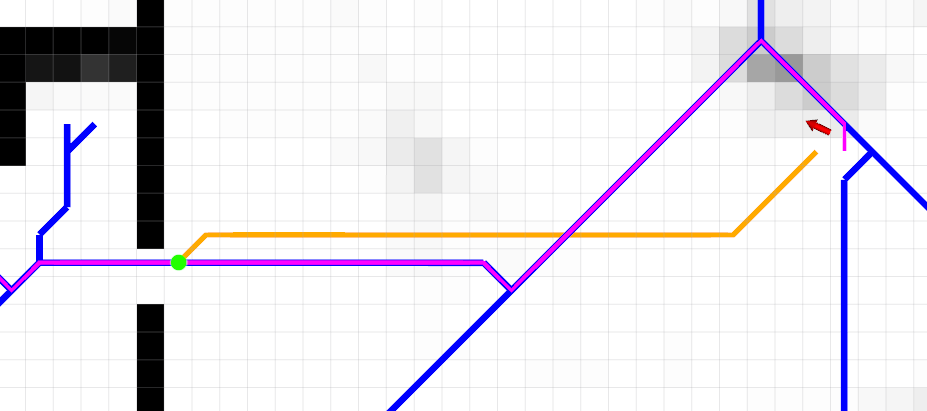
\includegraphics[width=1\linewidth]{imagenes/navjer/caso1/a.png}
  \caption[Planificación jerárquica.]{Planificación jerárquica. El GVD
    se indica con azul. En magenta se marca el camino original y en
    naranja el de bajo nivel, siendo el punto verde el primer
    subobjetivo sin completar del camino original. El vector rojo indica
    la posición y orientación del robot.
 }
  \label{fig:navjer}
\end{figure} 


\section{Construcción cooperativa del mapa}
% Durante la exploración la grilla de ocupación (seccion \ref{subsec:Grilla}) que
% representa el entorno explorado celdas  estado se puede determinar como
% ocupadas, libres y desconocidas

% Para una celda $c$ con estado desconocido, es equiprobable que $c$ este ocupada o 
% libre, siendo necesaria evidencia de
% que la celda esta ocupada ni de que esta libre, para que la celda cambie su
% estado ya sea a libre o a ocupado. En un escenario donde se comienza sin conocimiento sobre
% el entorno explorado y que el objetivo de la exploración es obtener
% informacion de dicho entorno, es posible decir que todas las celdas comienzan con estado desconocio 
% y el número de celdas en dicho estado decrece a lo largo que transcurre la
% exploración, a medida que se obtiene informacion (evidencia) sobre el entorno.


% A lo largo de la exploración se le asignan objetivos de exploración robots de
% la flota, con el propósito que los robots se dirijan a dichos objetivos y
% recopilen nueva información del entorno con sus sensores. Esta
% usada como mapa que representa el entorno explorado
 % que contiene toda la información obtenida del entorno
% explorado.

A lo largo de la exploración los robots utilizan sus sensores para recopilar
información del entorno. Esta información sensorial debe ser manejada para
aportar a la construcción del mapa, que es representado con una grilla de
ocupación (sección \ref{subsec:Grilla}) que centraliza toda la información del
entorno obtenida por los robots. A continuación se describe el proceso completo
desde que el robot obtiene información sensorial, hasta que esta impacta en el
mapa.

% El nodo
% \emph{Global\_costmap} fue configurado para que los valores de probabilidad de
% ocupación asociados a las celdas de la grilla que construye solo dependan de la
% ultima evidencia sensorial disponible para cada celda.

Cada robot está constantemente recopilando información del entorno a través de
sus sensores y enviando dicha información al nodo \gls{ROS}
\emph{global\_costmap} de su módulo \emph{Move Base} (sección
\ref{subsec:move_base}). Al recibir información sensorial el nodo
\emph{global\_costmap} envía una actualización al módulo \emph{combinador de
mapas} que consiste en el conjunto de las celdas $c$ que están en el alcance de
la información sensorial recibida y sus probabilidades $P(c | x_t,z_t)$ asociadas. El
valor de $P(c|x_t,z_t)$ indica la probabilidad de que una celda
$c$ esté ocupada dada la información sensorial $z_t$ obtenida desde la posición
$x_t$. Dependiendo de la evidencia que aporte $(x_t,z_t)$ sobre el estado de
$c$, la probabilidad $P(c|x_t,z_t)$ puede tomar uno de los siguientes
valores: $p_{prior} = 0.5$ si no aporta evidencia, $p_{occ} = 0.55$ si la
evidencia indica que la celda está ocupada y $p_{free} = 0.45$ si la evidencia
indica que la celda está libre. Estos valores de probabilidad son los que se
encuentran presentes en la solución desarrollada y se determinaron de forma
experimental asegurando que cumplen con \eqref{eq:probs} según se establece en
\cite{stachniss2009robotic}.\todohint{quedo bien? (desde -Dependiendo de la evidencia-)}

\begin{equation}\label{eq:probs}
  0 < p_{free} < p_{prior} < p_{occ} < 1
\end{equation}

% \todoerror[inline]{Acarar que los determine de forma experimental y que me base
% en lo de stanchis | El libro de Stachniss no especifica más que $0 \leq pfree < pprior < pocc \leq 1$ y que $pprior$
% suele usar como $0.5$. Y mismo los $\leq$ son cuestionables, pro ejemplo si
% $pfree = 0$ en la regla de update queda una division entre $0$. La verdad es
% que los valores principalmente los determine de forma experimental (mi
% respuesta a esas preguntas sería que 0 y 1 no funcionaron bien). La intuición
% que me quedo de las pruebas que hice para determinar esos valores es que
% valores de $pfree$ y $pocc$ más cercanos al $0.5$ logran que la historia de
% evidencia tenga más peso y los más alejados de $0.5$ que la evidencia reciente
% sea la que tenga más peso. Poner la intuición sin fundamento real no creo que
% este bueno, y buscar más por alguna fuente con una expedición o probar la
% intuición matemáticamente no creo que valga la pena. De última puedo aclarar
% que los valores se determinaron de forma experimental. | justificaría un poco
% más el uso de esos valores. por qué no 0.0 y 1.0, p.e.}

% Cuando la grilla de ocupación del nodo \emph{global\_costmap} de un robot

% Dado que cada \emph{global\_costmap} construye una grilla de ocupación que solo
% considera los datos sensoriales del robot en el que ejecuta, estas se deben
% combinar en una única grilla de ocupación que centralice toda la información
% recopilada del entorno. Esto se logra configurando

% Cuando la grilla de ocupación del nodo \emph{global\_costmap} de un robot
% experimenta cambios se envía las porciones que fueron actualizadas al módulo
% \emph{combinador de mapas}. Dichas porciones consisten en el conjunto de celdas
% de la grilla que fueron modificadas y sus nuevos valores de ocupación.

% las porciones que fueron actualizadas . Dichas porciones consisten en .
% , celda a celda


Cuando el módulo \emph{combinador de mapas} recibe una actualización, este
aplica la regla de actualización presentada en \cite{stachniss2009robotic} para
integrar la información recibida al mapa que mantiene, representado por una
grilla de ocupación que concentra toda la información proporcionada por los
robots. La regla de actualización para una celda $c$ está dada por
(\ref{eq:updateRule}) donde $P(c|x_{1:t-1},z_{1:t-1})$ es la probabilidad
anterior a la actualización, $P(c | x_t,z_t)$ es la probabilidad en la
actualización recibida y  $P(c|x_{1:t},z_{1:t})$ es la probabilidad luego de la
actualización. En la figura \ref{fig:mappingUpRule} se muestra un ejemplo de la
aplicación de esta regla de actualización. 

\begin{equation}
  P(c|x_{1:t},z_{1:t}) =\left( 1 + \frac{1 - P(c | x_t,z_t)}{P(c|x_t,z_t)} \frac{1 - P(c|x_{1:t-1},z_{1:t-1})}{P(c|x_{1:t-1},z_{1:t-1})} \right)^{-1}
\label{eq:updateRule}
\end{equation}

% Notar que en el ejemplo de la figura los mapas
% intermedios son distintos a los descritos en esta sección.

Luego de que el módulo \emph{combinador de mapas} integra toda la información
recibida en una actualización, este envía la porción actualizada del mapa a los
diversos módulos (sección \ref{sec:arqui}) que requieren un mapa
completo del entorno explorado.

\begin{figure}[H]
  \center
  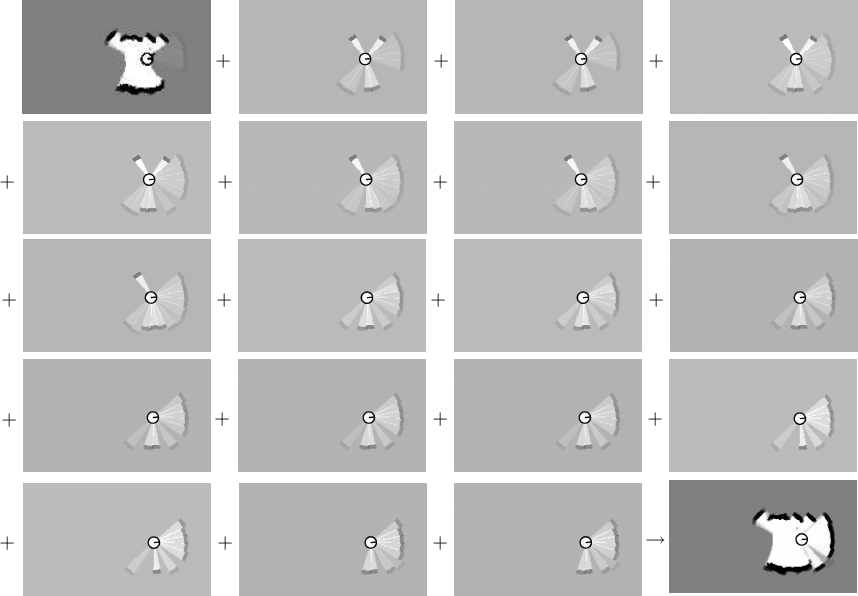
\includegraphics[width=1.00\linewidth]{imagenes/occgridUpdate.png}
  \caption[Aplicación de la regla de actualización propuesta en
  \cite{stachniss2009robotic} en un corredor.]{Aplicación de la
    regla de actualización propuesta en \cite{stachniss2009robotic} en un
    corredor. En la esquina superior izquierda muestra el mapa inicial y
    en la inferior derecha el mapa resultante. Los mapas intermedios corresponden a las actualizaciones integradas. Extraída de
  \cite{stachniss2009robotic}. }
  \label{fig:mappingUpRule}
\end{figure} 

% Y por otro lado como estas actualizaciones se integra (el método que se describe en \cite{stachniss2009robotic}).
% notando que solo se considera los datos sensoriales
% aportados  el robot

% si
% esto genera un cambio en la grilla, este cambio se informa al módulo
% \emph{combinador de mapas}. 

% robot completa un objetivo de exploración este recopila nueva
% informacion del entorno a partir de sus sensores

% Comentar como funcina el map merger:

% las actualizaciones, que las da el stack de navegacion, lo que esto implica
% (los datos de los sensores se procesan en celdas), que son incrementales (solo
% porcion del mapa) tanto la entradas como las salidas

%%%%%%%%%%%%%%%%%%%%%%%%%%%%%%%%%%%%%%%%%%%%%%%%%%%%%%%%%%%%%%%%%%%%%%%%%%%%%%%%%%%%%%
% basura de planificación
% Resumiendo, la planificación jerarquica cosnsiste en utlizar el camino original
% para determinar los subobjetivos ubicados en las transicisiones entre los segmentos
% del camino y \emph{Move Base} para navegar dentro de los segmentos hacia dichas
% transiciones. 

% solo utilizar la información topologica contenida en
% los caminos originales generados sobre el GVD.

% (en su mayor parte compuesto por centros de celdas pertencientes a GVD) p
% que son más
% eficientes computacionalmente que los generados sobre todo el espacio libre de
% la grilla, sin las desventajas.
% no trivales se calcula sobre las celdas pertencientes al GVD, lo cual tiene
% menor costo computacional que considerar todo el espacio libre de la grilla de
% coupacion eficiente calcular.



% La ventaja de aplicar esta tecnica es que hace posible utlizar
% los caminos , 

% caminos sobre el GVD, pero los caminos resultantes pueden ser innecesariamente
% largos, mientras que \emph{Move Base} con la configuracion correcta, permite
% ejecutar de forma eficiente caminos cercanos a los lineales. De esta manera se
% aporvecha la eficiencia del calaculo de caminos sobre el GVD, y se evitan los
% desvios que dichos camnios tienen, solo utlizando de estos los subobjetivos que
% se ubican en portales, 


% del camino y \emph{Move Base} para navegar dentro de los segmentos hacia dichas
% transiciones. La ventaja de aplicar esta tecnica es que hace posible utlizar los camnios
% no trivales se calcula sobre las celdas pertencientes al GVD, lo cual tiene
% menor costo computacional que considerar todo el espacio libre de la grilla de
% coupacion eficiente calcular.


% Recordando que los caminos originales se contruyen principalmente sobre el GVD,
% los niveles de jerarquia son do

% Por e dado un valor de $\mli{DistNs}$ más grande que elPara ejemp esto  esto porque los subobjetivos
% para los cuales exite una línea  

%   \item Existe una línea recta de grosor minDesiredDistance que lo conectan con el
%     robot sin solaparse con ningun obstaculo y tampoco tienen obtaculos a minDesiredDistance. 
%   \item Esta a meno de una distancia Z (Z puede estar entre forcedCompletionTolerance y alcance de sensado)


% Lo que se suele obtener en entornos estructurados es que los robots se mueven
% libremente en el interior los segmentos, mientras que para pasar de segmento a
% segmento utiliza el gvd para pasar por los pasajes estrechos que consituyen las
% puertas.

% En el caso de un Y pequeño se tiene una navegacion que sigue de forma más estricta al GVD.



% Los objetivos triviales se definen como los objetivos para los cuales el
% segmento de recta que existe entre el robot y el objetivo no contiene
% obstaculos, de lo contrario el objetivo es no trivial. Para determniar esto, se
% discretiza el segmento de recta en celdas \cite{foleyphillips} y se comprueba
% en el mapa global (grilla de ocupacion) almacenado en el robot, alguna de las
% celdas tiene un estado ocupado.

% El camino en objetivos triviales se determina como dicho segmento de recta que
% existe entre el robot y el objetivo, que se encuentra libre de obstaculos. 




% Este camino se divide subobjetivos y objtivos. El
% objetivo es el objetivo asignado, ubicado al final del camino. Por otro lado
% subobjetivos, son puntos intermedios correspondientes a centros de celda

% planificar como llegar a dicho objetivo. 


% Luego de que la central concluye el proceso a traves del cual determina que
% objetivo asignar a un robot  e informa dicha
% asignacion.  

% asignado a un objetivo el robot deberá llegar hasta el, para esto es necesario
% solucionar el este problema de planificación. La solución desarrollada aplica
% las ideas de planificación jerárquica presentadas en la sección
% \ref{subsec:mapas}, con el motivo de permitir una planificación eficiente sin
% resultar en caminos innecesariamente largos.




% Referenciar los tipos de caminos a la parte de la valuacion que habla de esto.

% Describier el proceso a detalle desde que llega un camino, y como este se va
% completando poco a poco hasta llegar al objetivo de exploración al final del
% camino.

% Tocar por arriba los mecanismos de recuperacion si queda facil.

% \subsection{Subobjetivo}
% Es un punto intermedio de un camino que lleva a un objetivo, el cual debe ser percibido por los sensores del robot

% Un subobjetivo se considera completo si:
% \begin{itemize}
%   \item Existe una línea recta de grosor minDesiredDistance que lo conectan con
%     el robot sin solaparse con ningun obstaculo y tampoco tienen obtaculos a
%     minDesiredDistance. 
%   \item Esta a meno de una distancia Y (Y puede estar entre
%     forcedCompletionTolerance y $\infty$)
% \end{itemize}
% O si:
% \begin{itemize}
%   \item Esta a menos de una diatancia forcedCompletionTolerance (mencionada en otra seccion, se puede ver de reorganizar luego)
% \end{itemize}

% \subsection{Objetivo}
% Es el punto final de un camino, debe ser percibidopor los sensores del robot

% Un objetivo se considera completo si:
% \begin{itemize}
%   \item Existe una línea recta de grosor minDesiredDistance que lo conectan con el
%     robot sin solaparse con ningun obstaculo y tampoco tienen obtaculos a minDesiredDistance. 
%   \item Esta a meno de una distancia Z (Z puede estar entre forcedCompletionTolerance y alcance de sensado)
% \end{itemize}

% O si:
% \begin{itemize}
%   \item Esta a menos de una diatancia forcedCompletionTolerance (mencionada en otra seccion, se puede ver de reorganizar luego)
% \end{itemize}

% \subsection{Objetivos triviales}
% Estos objetivos son los que tienen una línea recta de grosor X que lo conectan
% con el robot sin solaparse con ningun obstaculo y tampoco tienen obtaculos a
% X. X puede ser el maximo tamaño de una puerta o la minDesiredDistance.
% \begin{itemize}
%   \item Yo use un estimado del max tamaño de la puerta para evitar objetivos
%     triviales  que esten en un segmento distinto del que esta el robot
% \end{itemize}

% Estos objetivos tienen el trato especial de que los camninos planificados a
% estos no son sobre el GVD si no que consiten solo en el objetivo trivial.

% Esto facilita la navegacion cuando el camino al objetivo es muy facil, es decir es trivial.

% \subsection{Objetivos no triviales}

% Cuando el objetivo no es trivial lo que se hace es obtener un camnino utilizando el
% gvd como roadmap.

% Cada punto de este camnio es un subobjetivo menos el último que es el objetivo
% en si. El robot siempre se dirige al último subobjetivo/objetivo no competado.

% De esta forma notando las condiciones de complecion si Y es grande se tiene 
% navegacion libre (delegada a Move Base, el nivel bajo de la jerarquia) sobre
% zonas para las cuales no existen obtaculos mientras que se navega siguientdo el
% camnino seguro (provisto por el gvd, nivel alto de la jerarquia) cuando los
% objetivos son \say{no deseables} o \say{no seguros}.

% Lo que se suele obtener en entornos estructurados es que los robots se mueven
% libremente en el interior los segmentos, mientras que para pasar de segmento a
% segmento utiliza el gvd para pasar por los pasajes estrechos que consituyen las
% puertas.

% En el caso de un Y pequeño se tiene una navegacion que sigue de forma más estricta al GVD.

% % Entiendo que Y grande es mejor:
% %   `Una prueba para validar esto sería probar: Y en [50,10,5 2.5]`

% \subsection{Recupaeracion}

% \begin{itemize}
% \item Primero: "si tengo un objetivo activo y no estoy avanzando a el entoces intento recuperarme"
%   \begin{itemize}
%   \item Para saber el objetivo actual interceptar el next.
   
%   \item Si el objetivo cambia                           $=>$ reiniciar tiempo y distancia del último avance.

%   \item Si la distancia es menor a la del último avance $=>$ actualizar tiempo y distancia del último avance

%   \item Si pasan X segundo desde el último avance y el camino no esta completo =>
%     \begin{itemize}
%     \item Hacer recovery
%     \item reiniciar el timepo desde el último avance (dejar un rato antes del proximo recovery)
%     \end{itemize}
%   \end{itemize}

% \item Segundo: "Si según yo lo complete pero la central me dice que no esta completado seguramente no lo estoy viendo correctamente, intento recuperarme"
%   \begin{itemize}
%   \item Si se reasigna al objetivo => Hacer recovery
%   \end{itemize}
% \end{itemize}

% La recuperacion cosiste de:
% \begin{itemize}
%   \item  ir un poco para atras (en direccion opuesta al objetivo)
%   \item  esperar un tiempo estimando la llegada a la posicion a la que se fue en el punto anterior
%   \item  notificar a la central de la recuperacion para reasisgnar objetivos:
%   \begin{itemize}
%     \item Util por cambiar la pos del robot tanto en Primero como en Segundo
%     \item Util en segundo porque capaz ahora si se completo el objetivo
%   \end{itemize}
%   \item  Mientras la central no atienda al pedido volver al objetivo y eventualmente seguir con el camino
% \end{itemize}

%%%%%%%%%%%%%%%%%%%%%%%%%%%%%%%%%%%%%%%%%%%%%%%%%%%%%%%%%%%%%%%%%%%%%%%%%%%%%%%%%%%%%
% basura de GVD
% Dado esto se puede afirmar que $c_1$ y $c_2$ pertenecen al GVD si y solo si
% $oc_1\neq oc_2$ y no son adyacentes, 

% Hablar de la necesidad de encontrar las celdas base para lograr definir la
% líneas críticas y posteriormente lograr segmentar (seccion \ref{subsec:mapaTopGVDGrid}).

% Mencionar la solucion a la que se llego, y cual es la definicion de celda base.
% Dos caminos (I) mi definicion que separa los basis en sources y pseudosources. O (II)
% definir los basis como las celdas ocupadas que hacen que una celda pertenezca
% al GVD según lau (solo se neceita para puntos críticos incluidos en el GVD). 

% (II) tiene la ventaja que es facil de explicar y permite basarse en lo que ya
% esta bien fundamnetado (Lau), por otro lado (I) es lo que se implemento, pero
% puede ser dificil de explicar, sin tener mucho fundamento más que el
% generalizar y definir bien para el haberlo hecho asi. (puedo tomarme un tiempo
% para pensar en algun acaso claro y facil de epxlicar donde (I) esto funcione
% mejor pero no se)

% (I) aplica el criterio de siegwart-ming que capaz esta bueno que sea epxlicito.

% (I) permite comentar el tema de dist 1. (se puede mencionar en II tambien,
% diciendo que se hace eso pero que en realidad se saco si experimetnar el rido
% que dice que evita)

% Se puede intentar comentar todo en alto nivel

%%%%%%%%%%%%%

% Comentar como a partir de esta definicion de celda base, y las nociones de no
% adyacentes ni iguales entoces diferentes generadores (parrafo más abajo) se
% logra una nueva condicion de pertenencia al GVD, la cual esta más cercana a la
% definicion de GVD en el espacio continuo. (aunque aca cuidado, que tan distinta
% es al final? no se hace algo similar pero solo usando el obstaculo más
% cercano?) capaz puedo ir por ese lado y siendo más facil basarse en el trabajo
% de lau que redefinir sin mucho fundamento.

% Bueno hay una diferencias, la condicion de distancias de liu ming, y que no se
% permiten pseudosources adyacentes entre si. Ademas que se mantiene un registro
% de pseudosources.

% Son detalles que estan buenos para mi, porque son más generales mejor definidos
% pero no se que tanto puedo fundamentar su necesidad, y por lo tanto no se que
% tanto aporta dar toda la epxlicacion para lo que cuesta explicar y entender, creo que se
% puede epxlicar más facilmente con un solo obstaculo y esableciendo los oc que
% hicieron que pertenezca al GVD.

% fue necesario analizar el
% funcionamiento del algorimo.

% Hablar de que en \emph{brushfire dinamico} no se manejan los generadores de forma directa,

% Dado esto, 
% se decidio definir los puntos que base discretizados $\mli{BPD}_c$ 
% como las celdas obstaculizadas no adyacentes que generan la pertenecia
% de una celda $c$ al GVD.
% Establecido esto, es pertinente notar que la implementacion de \emph{brushfire
% dinamico} hecha en este proyecto difiere en la original en que esta almacena
% las celdas ocupadas que generan la pertenecia de un punto al GVD para ser
% utilizados posteriormente como puntos base.


% A lo largo de esta seccion se explicaran las conicidencia y cambios entre
% \emph{brushfire dinamico} y la variante de este implementada en este proyecto.

% \subsection{Algorimo general}

% \begin{algorithm}[H]
% \SetAlgoLined
% \SetKwProg{Fn}{Function}{}{}

% \Fn{establecerFuente(f)}{
%   $F_i := {f}$\\ 
%   $\mli{FP}_i := \emptyset$\\
%   $\mli{DD} := 0$\\
%   $removido := falso$
% }


% \Fn{removerObstaculo(oc)}{
%   $F_i := \emptyset$\\ 
%   $\mli{FP}_i := \emptyset$\\
%   $\mli{DD} := \infty$\\
%   $removido := verdadero$
% }
    
% \caption{Brushfire }
% \label{alg:DinBF}
% \end{algorithm}
% poner pseudocodigo de todo lo que hice basado en el de lau
% Si se sigue entendiendo lo de abajo sin esto me parece mejor evitarlo (muy similar a lau que ya se explico (sin pseudo pero la idea si) y la explicacion ocn pseudo puede llevar algunas carillas)

% \subsection{Pertenecia}
% La implemetacion realizada en proyecto mantiene las ondas conistentes e
% inconsistentes para el calulo incremental de mapas de distancia. Tambien
% mantiene la idea que las ondas inconsistentes remueven las celdas que atraviesan
% del GVD y la idea de que las celdas en las cuales las ondas consistentes se
% detienen y las celdas que causaron que se detengan son las celdas cuya
% pertenencia al GVD se comprueba.

% capaz prodria decir la def de pertenecia dado un choque de ondas, explicar que
% un choque de ondas siempre se da entre dos celdas, explicar el de lau, y el mio,
% estableciendo bien como es el tema de los pseudosources y las diff, dada la
% info que lleva la onda, etc. Aunque puede ser dificil dar ejemplos

% El cambio que se hace es en el criterio con el cual se comprueba la pertenencia
% de una celda. En el \emph{brushfire dinamico} original se hace EXPLICAR
% CON LO DE más ABAJO. En esta implementacion cambia, al existir un choque de
% ondas primero se establecen los pseudosources y luego de existir dos
% pseudosources no adjacentes entre si la celda pertenece.

% Explicar definicion de un pseudosource (SACAR DE LAS NOTAS), y porque esto termina siendo distinto
% que lo que se plantea en el \emph{brushfire dinamico} original.

% Capaz que explicar que el evitar generar si no hay dos basis no vecions es el evitar generar incorrectamente gvd en corredores diagonales. (aunque puede dar lugar a la discucion de que pasa si no es completamente diagonal, cosa que sospecho que puede dar problemas similares)

% Oportunidad de comentar que mejora sobre lau porque perminte generar gvd en
% lugares a dist 1 (ver bien que), cosa que lau no permite por resistencia al ruido pero que con el método actual no llevo mayores inconvenientes permitiendo generar gvd en grillas con el maximo tamaño de celda posible en el cual las puertas más chicas consisten de una unica celda ejemplo de algo asi: (esta en comentarios de latex)

%   mio            lau
% - - | - -      - - - - -
% - - | - -      - - - - -
% X X | X X  VS  X X - X X 
% - - | - -      - - - - -
% - - | - -      - - - - -

% Explicar que quizas se relacione al tema corredor de largo 2 que se va a explicar en \ref{subsec:filt}.

% \subsection{Filtrado}\label{subsec:filt}
% Los vetices que en una iteracion se determina que deben pertenecer al GVD según
% el criterio de pertenecia aplicado en las celdas en las cuales se detiene una
% onda consistente, pasan por un filtrado extra. Este filtrado busca evitar líneas
% discretizadas de dos celdas de grosor que violan la propiedad \say{sparceness}
% GVD.

% As discussed before, different paths on the Voronoi graph correspond to
% topologically different routes in the environment (sparceness property). To preserve this property
% for GVDs on grid maps, thin Voronoi lines, i.e., being one pixel wide, are
% desired.

% Spacrceness:Their application as roadmaps is an appealing technique for path
% planning, since they are “sparse” in the sense that different paths on the
% graph correspond to topologically different routes with respect to obstacles.
% This

% En el \emph{brushfire dinamico} original el filtrado se lleva a cabo haciendo
% uso de patrones con los cuales se comprueba si el GVD queda o no disconexo

% Our optional pruning step erodes 2-pixel-wide Voronoi lines. Therefore, all
% new Voronoi cells are inserted into a priority queue and processed by the
% pruning stage. The image operator patterns shown in Fig. 6 (solo poner
% 8-connected) match whenever the center cell s provides connectivity for one or
% more of its adjacent cells. In any pattern, a $1$ matches voro(s) = true, while
% $0$ stands for voro(s) = false, and empty fields are ignored. Where indicated
% by arrows, the same pattern is applied in all unique 90 degree rotations

% The second phase implements the actual pruning step. In increasing order of
% distance, the enqueued cells are iteratively popped from the priority queue. If
% such a cell has more than one neighbor on the GVD and is not required to keep
% the GVD connected, it can be removed from the GVD without affecting its
% topology. Again, this is tested using the image operator patterns: if none of
% the connectivity patterns match at the cell location, the cell is not required
% in the GVD.

% Enfasis en $P^8_1$ que indica que las celdas con un solo vecino deben pertenecer al GVD.

% En el caso de la implementacion del proyecto se comprueba si el GVD queda
% disconexo aplicando la tecnica presente en \cite{zhang1984fast},
% adicionalmente evitando filtrar celdas con una sola celda adyacente en el GVD
% y con 2 celdas ayacentes en el GVD si estas se detectan en un corredor.

% Explicar caso corredor(SACAR DE LAS NOTAS). comentar que no se considera en
% lau, quizas este es un problema que se arregla no permitiendo dist = 1. Aunque
% más analisis son necesarios

% \subsection{Limpieza de aristas}
% La limpieza de aristas es una tecnica aplicada solo en la implementación del
% proyecto esta permite generar GVD más limpios. 


% \subsection{Segmentacion}
% yo diria de 

% Creo que aca en realidad no habria que comentar mucho si es que hay que comentar, son las mismasideas que las comentadas en \ref{subsec:mapaTopGVD}.

% Quizas mencionar que se usa la descomposición en componentes conexas y como. 

% Mencionar el uso de sources y pseudosources para hacer líneas críticas. Discretizacion de líneas?

% Algunos resultados?

%%%%%%%%%%%%%%%%%%%%%%%%%%%%%%%%%%%%%%%%%%%%%%%%%%%%%%%%%%%%5

% basura de: \subsection{obtención de fronteras significativas basada en cubrimiento}

 %  \item Actualizar $\mli{FS_i}$ agregando $\mli{fs}$:

 %    $\mli{FS_i} := \mli{FS_i} \cup \{\mli{fs}\}$

 %  \item Actualizar $\mli{UF}$ removiendo todas las fronteras cubiertas por $\mli{fs}$:

 %    $\mli{UF} := \mli{UF} - \mli{RC}$

 %    Con $\mli{RC}=\{ f\in F_i : d_{\mli{fs}}(f) \leq rango\}$ las celdas recien
 %    cubiertas.

 %  \item Si $\mli{UF} \neq \emptyset$ volver a 1. de lo contrario devolver $FS_i$.
% \end{enumerate}



% Adicionalmente, se simepre que sea menor a $rango$ se usara la heuristica de 



% eleccion de
% $\mli{fs}$ debe considerar el resto de fronteras por cubrir y su cercania a los
% obtaculos, por ejemplo si $\mli{UF}$ es tan pequeño como para que se cubra
% completamente con una unica frontera significativa $\mli{fs}$ esta se deberia
% elegir para que este centrada en $\mli{UF}$.
%%acatoy
% Se asume que las fornteras más centradas se encuentran a una
% distancia $dCen = max\{ d_{\mli{FP}}(\mli{f}) : f\in\mli{UF} \}/2$ de
% $\mli{fp}$. 

% Combiando ambos factores se determina que el conjunto de fronteras
% significativas candidatas 

 % puede resumir como elegir una frontera $\mli{fs}$ que
% cubra 

% comienza desencolando una frontera $\mli{fp}$ de $\mli{FP}$
% que debe no estar cubierta todavia, por lo cual de estar cubierta se descarta y
% se vuelve a desencolar. 


% , si dicha forntera ya esta cubierta la eleccion se cancela 
% \begin{enumerate}
 %  \item 
 %  \item Actualizar $\mli{FS_i}$ agregando $\mli{fs}$:

 %    $\mli{FS_i} := \mli{FS_i} \cup \{\mli{fs}\}$

 %  \item Actualizar $\mli{UF}$ removiendo todas las fronteras cubiertas por $\mli{fs}$:

 %    $\mli{UF} := \mli{UF} - \mli{RC}$

 %    Con $\mli{RC}=\{ f\in F_i : d_{\mli{fs}}(f) \leq rango\}$ las celdas recien
 %    cubiertas.

 %  \item Si $\mli{UF} \neq \emptyset$ volver a 1. de lo contrario devolver $FS_i$.
% \end{enumerate}

%%%%%%%%%%%%%%%%%%%%%%%%%%%%%%%%%%%%%%%%%%%%%%%%%%%%%%%%%%%%%%%%%%%%%%%%%%%%%%%%%%%%%

% De los pasos presentados el primero es el principal y tambien el más complejo
% del algorimo.

% Los pasos del 2 al 4 no presentan ambigüedad, siendo el paso 1 en el que resta
% aclarar, especificamente lo que resta aclarar es el criterio con el que se
% elige la frontera significativa. La eleccion en un principio podria ser
% aleatoria y el algoritmo daria resultados validos, pero esto dejaria a la
% suerte la calidad de la solucion. La idea sería elegir de forma determinista a
% una frontera significativa buscando que cubra la mayor cantidad de fronteras
% mientras se evita cubrir nuevamente fronteras que ya sean cubiertas por otra
% frotntera significativa. 

% La tecnica desarrollada se basa en mantener una cola FIFO en donde se guardaran
% los proximas fronteras a cubrir $\mli{FP}$, 
% El proceso para elegir una nueva forntera significativa $\mli{fs}$ consiste en
% desencolar una frontera $\mli{FP}$ de $\mli{FP}$ para posteriomente determinar
% el conjunto de fronteras significativas candidatas $\mli{FSC}$ como las
% fronteras sin cubrir desde las cuales se cubre a $\mli{FP}$ estando lo más
% alejadas posible de esta, es decir, que $\mli{FSC}$ %$= \{f\in \mli{UF} : d_{\mli{fs}}(\mli{FP})= rango$\}
% sera el conjunto de celdas en $\mli{UF}$ que solapen con la circunferencia del
% circulo de radio $rango$ centrada en $\mli{FP}$ denotada como $\mathscr{C}(\mli{FP},rango)$.
% Para elegir una nueva frontera significativa $\mli{fs}$ se debe elegir una
% frontera de $\mli{FSC}$, que en esta propuesta se hace de forma arbitraria.


% Ahora resta tratar dos casos bordes, el primero es la inicializacion de
% $\mli{FP}$ cuando no existen fronteras adyacentes a obstaculos, cuando esto
% sucede para inciar el algorimo basta con agregar una unica frontera arbitraria
% de $F_i$ a $\mli{FP}$. El otro caso es el que se presenta si $\mli{FSC} = \emptyset$
% \todo{esto esta mal, en realidad esta mal desde antes cuando se presenta FSC, FSC busca que las candidatas queden centradas. Por lo que el radio puede ser menor al rango aunque haya una (o más) celda solapada conla circunferencia de radio rango}
% , es
% decir la circunferencia del circulo de radio $rango$ centrada en $\mli{FP}$ no
% se solapa con ninguna celdas en $\mli{UF}$. Cuando esto sucede lo que se hace
% es reducir el radio del circulo a $\frac{max\{ d_{\mli{FP}}(\mli{f}) :
% f\in\mli{UF} \}}{2}$ la divicion entre dos busca que la circunferencia se
% solape sobre el punto medio entre $\mli{FP}$  y la celda de $\mli{UF}$ más
% alejada de $\mli{FP}$, quedando la nueva frontera significativa centrada
% (figura ejemplo de esto).

% Para que el criterio de eleccion propuesto funcione de forma correcta es
% necesario agregar al paso 2 que  se deben encolar a $\mli{FP}$ todas las
% fronteras del siguiente conjunto $\{ f \in \mli{UF} : \exists c \in \mli{FS_i}
% - \mli{UF}, f \in ady(c)\}$ que no esten ya encoladas.

% $\mil{CF}$ de las fronteras
% cubiertas pos la nueva $\mli{fs}$, encolan a $\mil{FP}$ a las celdas de $


% elegir
% $\mli{fs}$ como uno de las 

% La condicion de distancia busca maximizar la
% cantidad de fronteras que cubre la nueva frontera significativa.

% EL algorimo se basa en la idea de que una buena distribucion de fronteras
% significativas deberia mantener en su mayor parte una distancia de $rango*2$
% entre cada frontera significativa, ya que esta es la distancia máxima que se
% puede tener para asegurar qu se cumpla el cubrimiento. 
